\documentclass{article}
%\usepackage[top=30pt,left=30pt,right=30pt]{geometry}
\usepackage[german,english]{babel}
\usepackage[utf8]{inputenc}
\usepackage{algpseudocode}
\usepackage{algorithm}
\usepackage{graphicx}
\usepackage{caption}
\usepackage{subcaption}
\usepackage{amsmath}
\usepackage{amssymb}
\usepackage{enumitem}
\usepackage{amsthm}
\usepackage{pxfonts}
\usepackage{wasysym}
\usepackage{framed}
\usepackage{xcolor}
\usepackage{makeidx}
\usepackage{csquotes}
\usepackage[pdfborder={0 0 0}]{hyperref}
\usepackage{stmaryrd}
\usepackage{titlesec}
\titleformat{\paragraph}{\normalfont\itshape}{}{}{}

\newtheorem{theorem}{Theorem}  \numberwithin{theorem}{section}
\newtheorem{problem}{Problem}  \numberwithin{problem}{section}
\newtheorem{example}{Example}  \numberwithin{example}{section}
\newtheorem*{hypothesis}{Hypothesis}%  \numberwithin{hypothesis}{section}
\newtheorem{definition}{Definition}  \numberwithin{definition}{section}
\newtheorem{lemma}{Lemma}  \numberwithin{lemma}{section}
\newtheorem*{claim}{Claim}%  \numberwithin{claim}{section}
\newtheorem{remark}{Remark}  \numberwithin{remark}{section}
\newtheorem*{corollary}{Corollary}%  \numberwithin{corollary}{section}
\newtheorem{proposition}{Proposition}  \numberwithin{proposition}{section}

\algnewcommand{\algorithmicgoto}{\textbf{go to}}%
\algnewcommand{\Goto}[1]{\algorithmicgoto~\ref{#1}}%
\algrenewcommand{\algorithmiccomment}[1]{\hskip2em$\triangleright$ {\footnotesize #1}}

% definitions
\newcommand{\drawing}[1]{%
 \begin{figure}[t]
  \begin{center}
   \includegraphics{#1}
  \end{center}
 \end{figure}
}
\newcommand{\pic}[2]{%
 \begin{figure}[t]
  \begin{center}
   \includegraphics{#1}
   \caption{#2}
  \end{center}
 \end{figure}
}
\newcommand{\set}[1]{\left\{#1\right\}}
\newcommand{\setdef}[2]{\left\{\left.#1\,\right|\,#2\right\}}
\newcommand{\angel}[1]{\left\langle#1\right\rangle}
\newcommand{\norm}[1]{\left\|#1\right\|}
\newcommand{\card}[1]{\left|#1\right|}
\newcommand{\given}[1]{\textbf{Given.} #1\par}
\newcommand{\find}[1]{\textbf{Find.} #1\par}
\newcommand{\dateref}[1]{\paragraph{\textit{This lecture took place on #1.}}}
\newcommand{\exist}{\;\exists\,}
\newcommand{\fall}{\;\forall\,}
\newcommand{\noproof}[1]{A proof for Theorem~\ref{#1} is not provided.}
\newcommand{\person}[1]{Mathematician~#1.}
\makeatletter
\newcommand{\xRightarrow}[2][]{\ext@arrow 0359\Rightarrowfill@{#1}{#2}}
\makeatother

\newcommand{\mtn}{(\mu\times\nu)} % mu times nu

\DeclareMathOperator{\rank}{rank}
\DeclareMathOperator{\detm}{det}
\DeclareMathOperator{\perm}{det}
\DeclareMathOperator{\sign}{sign}
\DeclareMathOperator{\degree}{deg}
\DeclareMathOperator{\prop}{probability}
\DeclareMathOperator{\argmax}{argmax}
\DeclareMathOperator{\argmin}{argmin}
\DeclareMathOperator{\vol}{vol}  % volume
\DeclareMathOperator*{\bigtimes}{\vartimes}

\makeatletter
\providecommand*{\dotcup}{%
  \mathbin{%
    \mathpalette\@dotcup{}%
  }%
}
\newcommand*{\@dotcup}[2]{%
  \ooalign{%
    $\m@th#1\cup$\cr
    \hidewidth$\m@th#1\cdot$\hidewidth
  }%
}
\makeatother


% metadata
\title{
  Measure and integration theory \\
  \large{Lecture notes, University of Graz} \\
  based on the lecture by Wolfgang Ring
}
\date{\today}
\author{Lukas Prokop}

% settings
\parindent0pt
\setlength{\parskip}{0.4\baselineskip}
%\setcounter{tocdepth}{2}

\makeindex

\begin{document}
\maketitle
\tableofcontents

\section{Elementary concepts and Riemann (Cauchy) integration}

\dateref{2017/10/04}
Lecturer: Wolfgang Ring

Literature:
\begin{enumerate}
  \item Knapp, \enquote{Basic Real Analysis}
  \item W. Rudin, \enquote{Real \& Complex Analysis}
  \item Bressoud, \enquote{A Radical Approach to Lebesgue Integral}
\end{enumerate}

\begin{problem}[Containment problem]
  Given a geometric size (triangle, octaeder, sphere, $M \subseteq \mathbb R^n$).
  Find the corresponding volume.
\end{problem}

We desire certain properties:
\begin{itemize}
  \item $A \subseteq \mathbb R^n$
  \item Let $\mu(A)$ be the volume of $A$. $\mu(A)$ satisfies $\mu(A) \geq 0$.
  \item Let $A \cap B \neq \emptyset$. $\mu(A \cup B) = \mu(A) + \mu(B)$ (\enquote{additivity} property, $\sigma$-additivity)
\end{itemize}

\begin{theorem}
  The monotonicity property follows immediately: %(follows from additivity)
  \[ A \subseteq A' \implies \mu(A) \leq \mu(A') \]
\end{theorem}
\begin{proof}
  \[ A' = A \dotcup (A' \setminus A) \]
  \[ \mu(A') = \mu(A) + \underbrace{\mu(A' \setminus A)}_{\geq 0} \]
\end{proof}

\begin{figure}[!h]
  \begin{center}
    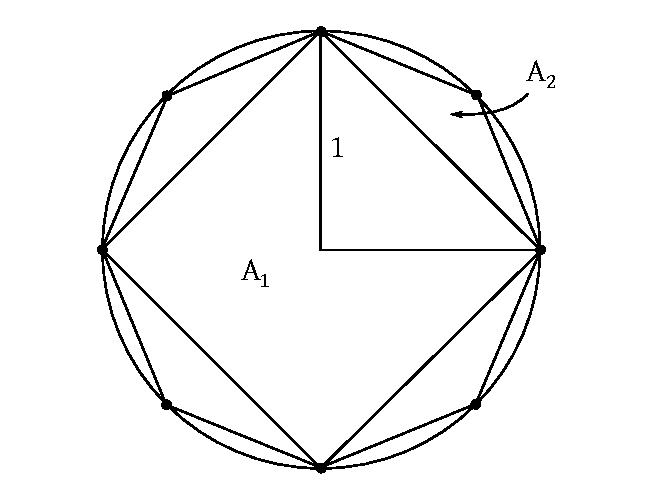
\includegraphics[width=0.5\textwidth]{img/12_area.pdf}
    \caption{
      Given a circle of radius 1.
      $A_1$ is the rectangle. $A_2$ is an octaeder inside the circle.
      Let's assume we know the volume of these objects.
      Can we assign a volume to the circle?
      This illustrates the containment volume problem.
    }
  \end{center}
\end{figure}

We desire the following property:
\[ A_n \subseteq A_{n+1} \land A = \bigcup_{n=1}^\infty A_n \]
\[ \implies \lim_{n\to\infty} \mu(A_n) = \mu(A) \]

\subsection{Limes considerations}

We consider countable, infinite processes
and use $sigma$-additivity.
\[ \left(A_n\right)_{n \in \mathbb N} \qquad A_n \cap A_m = \emptyset \text{ for } n \neq m \]
\[ \mu\left(\bigcup_{n=1}^\infty A_n\right) = \sum_{n=1}^\infty \mu(A_n) \]

Now we discuss another desirable property. Let $l = [a,b]$.
% an interval is in mathbb R, so it is "uncountable infinite"
\[ l = \bigcup_{a \leq x \leq b} \{x\} \]
\[ \mu([a,b]) = b - a = \sum_{a \leq x \leq b} \mu(\set{x}) = 0 \]
% TODO why zero?
Informally speaking, \enquote{points should not have any content}.

\begin{enumerate}
  \item How do we define a (or \emph{the}) volume?
        (a structure of Henry Lebesgue)
  \item Which sets are assigned some volume?
\end{enumerate}

\subsection{Banach-Tarski paradox}

\[ K: \mathbb R^n \mapsto \mathbb R^n \text{ with } K(x) = \mathcal O x + v \]
where $\mathcal O \in \mathcal O(n)$ and $\mathcal O$ is an orthogonal matrix.
$K$ is a congruence map.

\[ \mu(A) = \mu(K(A)) \quad \forall A \]

We parameterize $K$ with $\mathcal O = \begin{bmatrix} 0 \\ 0 \\ 0 \end{bmatrix}$ and $v = 1$.
\[ A = K(\begin{bmatrix} 0 \\ 0 \\ 0 \end{bmatrix}, 1) \subseteq \mathbb R^3 \]
\[ K = K(\begin{bmatrix} 0 \\ 0 \\ 0 \end{bmatrix}, 1) \cup K\left(\begin{bmatrix} 0 \\ 0 \\ 3 \end{bmatrix}, 1\right) \]

\begin{figure}[!h]
  \begin{center}
    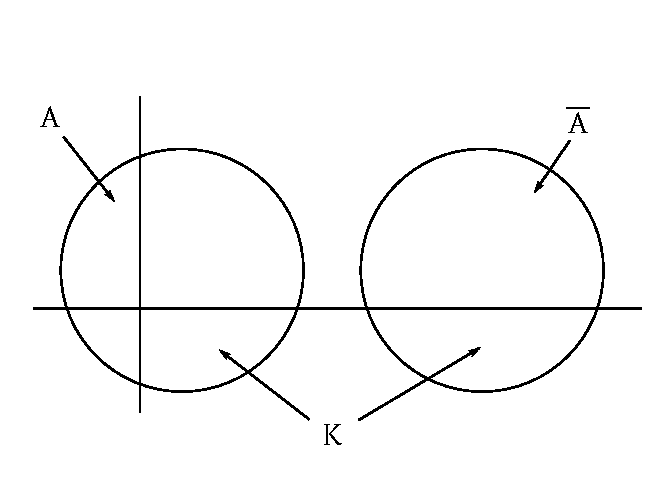
\includegraphics[width=0.5\textwidth]{img/08_bt_paradox.pdf}
    \caption{Banach Tarski paradox}
  \end{center}
\end{figure}

The following sets exist:
\begin{itemize}
  \item $A_1, A_2, \ldots, A_n \subseteq A$
  \item $B_1, B_2, \ldots, B_n \subseteq K$
\end{itemize}

\begin{align*}
  A_i \cap A_j = \emptyset \text{ for } i \neq j: \bigcup_{j=1}^k A_j = A \\
  B_i \cap B_j = \emptyset \text{ for } i \neq j: \bigcup_{j=1}^k B_j = K
\end{align*}
$B_j$ and $A_j$ are congruent for $j=1,\ldots,k$.
$A_j$ and $B_j$ cannot have volumes! % TODO: why?

It is not possible to assign an additive volme to every set.
Our goal is to create the \emph{largest} class of sets that do have volumes.

Volume is a measure.

\subsection{Cauchy integral}

\emph{Why are we not (entirely) confident with the Cauchy integral?}

\begin{itemize}
  \item Cauchy integration is defined on limited intervals:
    \[ \int_a^b f(t) \, dt \qquad a \leq b \qquad a,b \in \mathbb R \]
    \begin{align*}
      \int_1^\infty \frac{1}{x^2} \, dx
        &= \lim_{M\to\infty} \int_1^M \frac{1}{x^2} \, dx \qquad \text{\emph{improper integral, boundary process}} \\
        &= \lim_{M\to\infty} \lim_{n\to 0} \int_1^M t_n^M(x) \, dx
    \end{align*}
    It is desirable to compute $\int_{-\infty}^\infty f(x) \, dx$ directly.
  \item Limit theorems:
    Cauchy: $f_n \to f$ is uniform on $[a,b]$ ($f_n$ converge towards $f$ uniformly in interval $[a,b]$).
    Let $f_n$, $f$ be regulated functions. Then,
    \[ \lim_{n\to\infty} \int_a^b f_n(x) \, dx = \int_a^b f(x) \, dx = \int_a^b \lim_{n\to\infty} f_n(x) \, dx \]

    \begin{example}
      \[ f_n(x) = nxe^{-nx^2} \]
      Let $[0,1]$ be an integration interval. $f_n(0) = 0 \to 0$.
      Let $0 < x \leq 1$. Then it holds that $\lim_{n\to\infty} nxe^{-nx^2} = 0$.
      \[ f_n(x) \to 0 \qquad \forall x \in (0,1] \]
      Hence, $f_n \to 0$ is pointwise on $[0,1]$.
      \[ \lim_{n\to\infty} \int_0^1 f_n(x) \, dx \stackrel{?}{=} \int_0^1 \underbrace{f(x)}_{=0} \, dx = 0 \]
      \[ \int_0^1 nx \cdot e^{-nx^2} \, dx = \left.-\frac12 \cdot e^{-nx^2} \right|_0^1 = \underbrace{-\frac12 e^{-n}}{\to 0} + \frac12 \to \frac12 \]
      \[ \left(-\frac12 e^{-nx^2}\right) \]
    \end{example}

    \begin{example}
      \[ g_n(x) = \frac{n^2 x}{1 + n^3 x^2} \text{ on } [0,1] \]
      \[ \forall x \in [0,1]: \lim_{n\to\infty} g_n(x) = 0 \checkmark \text{ non-uniform} \] % amssymb
      \[ x_n = \frac1n \qquad g_n(x_n) = \frac{n^2 \cdot \frac1n}{1 + n^3 \cdot \frac{1}{n^2}} = \frac{n}{1+n} = \frac{1}{1 + \frac1n} \geq \frac12 \text{ for } n \geq 1 \]
      \[ \underbrace{\frac1{2n} \int_0^1 \frac{2 n^3 x}{1 + n} \, dx}_{\int_0^1 g_n(x) \, dx} = \left. \frac1{2n} \ln \left(1 + n^3 x^2\right) \right|_0^1 = \frac1{2n} \ln(1 + n^3) \to 0 \]
      \[ \lim_{n \to \infty} \int_0^1 g_n(x) \, dx = \int_0^1 g(x) \, dx \]
    \end{example}

  \item Fundamental theorem of Calculus (dt. Hauptsatz der Differential- und Integralrechnung):
    \[ f: [0,1] \to \mathbb R \qquad \frac{d}{dx} \left[ \int_0^x f(\xi) \, d\xi \right] = f(x) \]
    \[ f: [a,b] \to \mathbb R \text{ is a regulated function} \]
    \[ \forall x \in (a,b) \text{ exist } \lim_{\xi\to x^+} f(\xi) \text{ and } \lim_{\xi \to x^-} f(\xi) \]
    Fundamental theorem:
    \[ \left(\int_a^x f(\xi) \, d\xi\right)'_+ = \lim_{\xi \to x^+} f(\xi) \]
    \[ \left(\int_a^x f(\xi) \, d\xi\right)'_- = \lim_{\xi \to x^-} f(\xi) \]
    \begin{example}
      \[
        g(x) = \begin{cases}
          0 & x \in (0,1] \setminus \mathbb Q \cup \{0\} \\
          \frac1q & x = \frac{p}{q} \in \mathbb Q, \operatorname{gcd}(p,q) = 1
        \end{cases}
      \]
      \[ g(\frac1\pi) = 0; g\left(\frac{17}{24}\right) = \frac1{24} \]
      It holds: $g$ is a regulated function.
      \[ \forall x \in [0,1] \text{ exist one-sided limits} \]
      \[ \lim_{\xi \to x^+} g(x) = 0 \qquad \lim_{\xi \to x^-} g(x) = 0 \]
      If $x \in (0,1] \setminus \mathbb Q \qquad \xi_n \to x \qquad \xi_n \in (0,1] \setminus \mathbb Q \implies g(\xi_n) = 0$.
      \[ g(x) = 0: \xi_n = \frac{p_n}{q_n} \implies g_n \to \infty \implies g(\xi_n) = \frac{1}{q_n} \to 0 \]
      \[ x \in \mathbb Q, x = \frac{p}{q}, \xi_n \in (0,1] \setminus \mathbb Q \implies g(\xi_n) = 0 \to 0 \]
      \[ \xi_n = \frac{p_n}{q_n} = \frac{p}{q} \implies g_n \to \infty \text{ and } g(\xi_n) = \frac{1}{q_n} \to 0 \]
      \[ \left|\frac{p_n}{q_n} - \frac{p}{q}\right| < \varepsilon \implies 1 \leq \left| p_nq - q_n p\right| < \varepsilon q_n q \implies q_n > \frac{1}{\varepsilon \cdot q} \implies \infty \text{ for } \varepsilon \to 0 \]
    \end{example}
\end{itemize}

\section{Abstract measure theory}

\dateref{2017/10/06}

We want to:
\begin{itemize}
  \item define abstract structures constructing the integral
  \item later: specific construction on $\mathbb R^n$ (Lebesgue measure and integral)
\end{itemize}

\subsection{Topology on $X$}

\begin{definition}
  \index{Topology on $X$}
  Let $X \neq \emptyset$ be an arbitrary set.
  $\mathcal T \subseteq \mathcal P(X)$ is called a \emph{topology on $X$} if
  \begin{enumerate}
    \item $\emptyset \in \mathcal T$; $X \in \mathcal T$
    \item $\mathcal O_i \in \mathcal T$ for $i \in I \implies \bigcup_{i \in I} \mathcal O_i \in \mathcal T$
    \item $\mathcal O_1, \mathcal O_2 \in \mathcal T \implies \mathcal O_1 \cap \mathcal O_2 \in \mathcal T$
  \end{enumerate}
  $\mathcal P$ denotes the power set. Properties 2 and 3 hold for 2 or an arbitrary set of elements. \\
  \index{Open set in $X$}
  $\mathcal O \in \mathcal T$ is called \emph{open set in $X$} (in terms of chosen topology $\mathcal T$).
  $\mathcal T = \set{\emptyset, X}$ is the so-called \emph{indiscrete space on $X$} (or \enquote{trivial topology on $X$}).
  $\mathcal T = \mathcal P(X)$ is a (discrete) topology on $X$.
\end{definition}

\begin{quote}
  If you have a discrete conversation, you are disconnected from the society.
  Just like the points are distant from $P(X)$.
  Hence, discrete topologies are few elements in privacy.
  Indiscrete topologies include everybody (the society).
\end{quote}

We want to reach the definition of open sets in metric spaces (but we are not there yet).
In metric space $\mathbb R^n$, open sets are defined as:
\[ \mathcal O \subset \mathbb R^n \Leftrightarrow \forall x \in \mathcal O \exists r > 0: B(x,r) \subseteq \mathcal O \]
This holds in every metric space. Compare with Figure~\ref{img:topology}.

\begin{figure}[!h]
  \begin{center}
    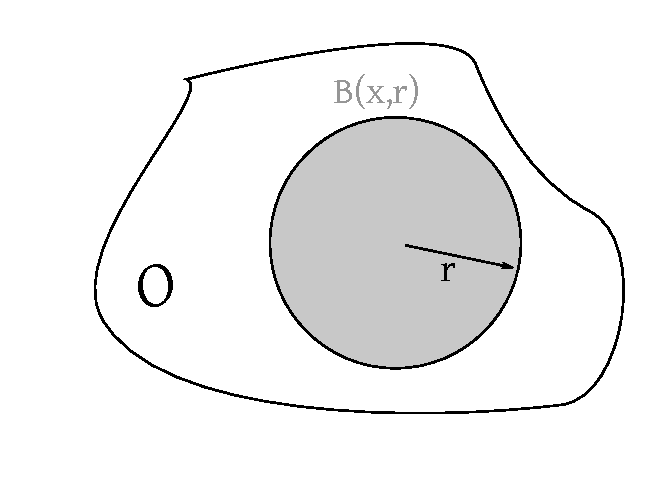
\includegraphics[width=0.5\textwidth]{img/01_topology.pdf}
    \caption{Topology}
    \label{img:topology}
  \end{center}
\end{figure}

\subsection{Set algebra}

\begin{definition}\label{def:setalgebra}
  \index{Set algebra}
  $\mathcal A \subseteq \mathcal P(X)$ is called \emph{(set) algebra on $X \neq 0$} if
  \begin{enumerate}
    \item $\mathcal O \in \mathcal A$, $x \in \mathcal A$
    \item $\forall A,B \in \mathcal A \implies A \cap B \in \mathcal A$
    \item $\forall A \in \mathcal A \implies \underbrace{(X \setminus \mathcal A)}_{\coloneqq A^C} \in \mathcal A$
  \end{enumerate}
\end{definition}
$\mathcal T$ is closed in terms of union and finite intersection.
$\mathcal A$ is closed in terms of union and complement.

\begin{corollary}
  Let $A,B \in \mathcal A$. Then,
  \[ A \cap B = \underbrace{(\underbrace{\underbrace{A^C}_{\in \mathcal A} \cup \underbrace{B^C}_{\in \mathcal A}}_{\in \mathcal A})}_{\in \mathcal A} \]
  Hence, $\mathcal A$ is closed under finite intersection.
\end{corollary}
\begin{corollary}
  \begin{align*}
    A \triangle B
      &= (A \cup B) \setminus (A \cap B) \\
      &= \underbrace{(A \cap \underbrace{B^C}_{\in \mathcal A})}_{\in \mathcal A} \cup \underbrace{(B \cap \underbrace{A^C}_{\in \mathcal A})}_{\in \mathcal A} \in \mathcal A \\
    A \setminus B &= A \cap B^C \in \mathcal A
  \end{align*}
\end{corollary}

$(\mathcal A, \cup, \cap)$ is a boolean algebra.

\subsection[Sigma-algebra]{$\sigma$-algebra}

\begin{definition}
  \index{$\sigma$-algebra on $X$}
  \index{Sigma-algebra on $X$}
  $\mathcal A$ is called \emph{$\sigma$-algebra on $X$} if we take the definition of a set algebra on $X$ (see page~\pageref{def:setalgebra})
  and replace the second criterion with
  \[ \forall (A_n)_{n \in \mathbb N} \text{ with } A_n \in \mathcal A \implies \bigcup_{n=1}^\infty A_n \in \mathcal A \]
\end{definition}

$\mathcal A$ is closed under finite union.
$\sigma$-algebra is a fundamental concept to define a measure.

$\mathcal A$ is closed under intersection of $\sigma$-intersection (i.e. infinite intersection).
\[ A_n \in \mathcal A \implies \bigcap_{n=1}^\infty A_n = \left(\overbrace{\bigcup_{n=1}^\infty \underbrace{A_n^C}_{\in \mathcal A}}^{\in \mathcal A}\right)^C \in \mathcal A \]

\subsection{Set ring}

\begin{definition}
  \index{Set ring}
  $R \subseteq \mathcal P(X)$ is \emph{(set) ring} if it satisfies,
  \begin{enumerate}
    \item $A, B \in R \implies A \cap B \in R$
    \item $A, B \in R \implies A \setminus B = A \cap B^C \in R$
  \end{enumerate}
\end{definition}

\subsection[Sigma-ring]{$\sigma$-ring}

\begin{definition}
  \index{Sigma-ring}
  $R \subseteq P(X)$ is called \emph{$\sigma$-ring} if it satisfies,
  \begin{enumerate}
    \item $\forall (A_n)_{n \in \mathbb N}: A_n \in R \implies \bigcup_{n=1}^\infty A_n \in R$
    \item $A, B \in R \implies A \setminus B = A \cap B^C \in R$
  \end{enumerate}
\end{definition}

Every algebra is also a ring. Every $\sigma$-algebra is also a $\sigma$-ring.

\subsection{Abstract cuboid}

\begin{definition}
  Let $X = \mathbb R^n$, $\alpha_i, \beta_i \in \mathbb R$ ($i=1,\ldots,n$).
  We let $[\alpha_i, \beta_i) = \set{x \in \mathbb R: \alpha_i \leq x \land x < \beta_i}$.
  $[\alpha_i, \beta_i) = \emptyset$ if $\alpha_i \geq \beta_i$.
  We call $Q$ \emph{abstract cuboid}, if it satisfies,
  \begin{align*}
    Q &= [\alpha_1, \beta_1) \times [\alpha_2, \beta_2) \times \ldots \times [\alpha_n, \beta_n) \\
      &= \bigtimes_{i=1}^n [\alpha_i, \beta_i) \subseteq \mathbb R^n  % TODO: huge is invalid in mathmode
  \end{align*}
  $Q = \emptyset$ if $\alpha_i \geq \beta_i$ for some $i \in \set{1,\ldots,n}$.
  Recall that, by definition, $A \times B = \emptyset$ for $A = \emptyset \lor B = \emptyset$.
  \[ W \coloneqq \set{Q \subseteq \mathbb R^n: Q = {\bigtimes}_{i=1}^n [\alpha_i, \beta_i)} \subseteq \mathcal P(\mathbb R^n) \]
  % It is a subset, because points cannot be represented by half-open intervals.
  % Additionally the parameters $\alpha_i$ and $\beta_i$ are not yet decided. Hence, we cannot determine whether it is \subseteq or \subseteqq
  Compare with Figure~\ref{img:cuboid}.
  \[ R_W = \setdef{V = \bigcup_{j=1}^m Q_j}{m \in \mathbb N \land Q_j \in W \text{ for } j = 1,\ldots,m} \]
  $R_W$ is the set of unions of half-open abstract cuboids.
\end{definition}

\begin{figure}[!h]
  \begin{center}
    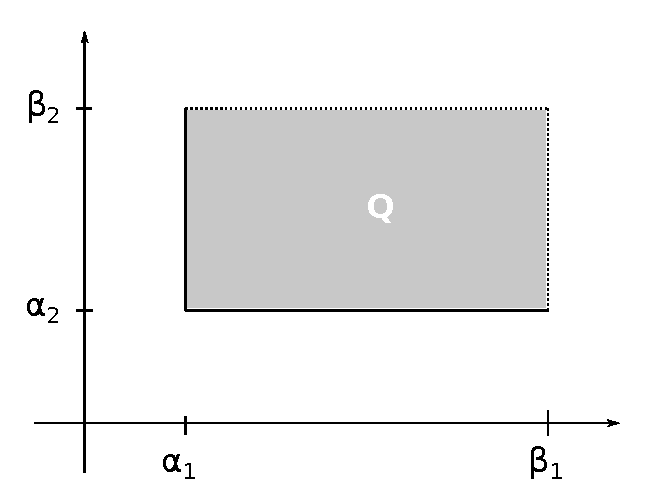
\includegraphics[width=0.5\textwidth]{img/02_cuboid.pdf}
    \caption{Abstract cuboid}
    \label{img:cuboid}
  \end{center}
  \begin{center}
    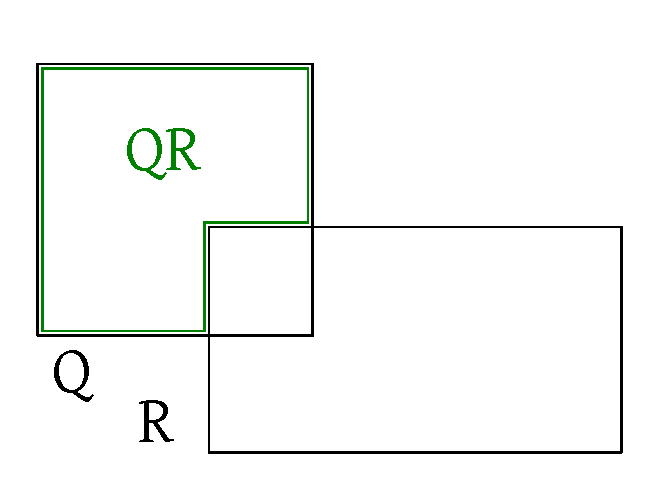
\includegraphics[width=0.5\textwidth]{img/02_lemma1a.pdf}
    \caption{Illustration that the subtraction of cuboid $R$ from $Q$ gives another structure $QR$ describable by two cuboids}
    \label{img:lemma1a}
  \end{center}
  \begin{center}
    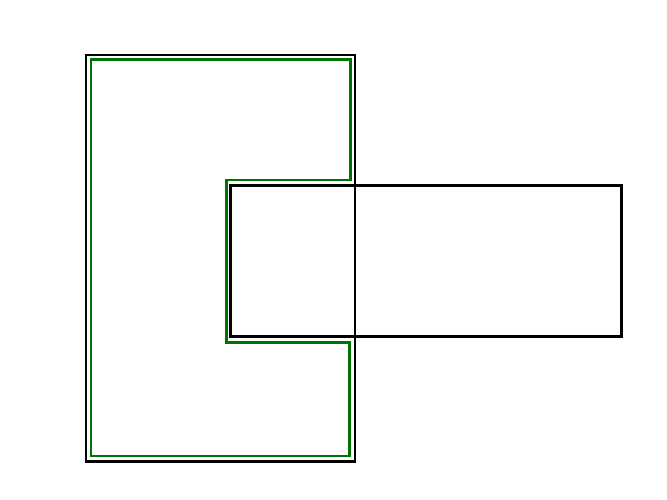
\includegraphics[width=0.5\textwidth]{img/02_lemma1b.pdf}
    \caption{Also this subtraction result is describable as union of 3 cuboids}
    \label{img:lemma1b}
  \end{center}
\end{figure}

\begin{lemma}
  \label{l:one}
  If $V_1,\ldots,V_n \in R_W$, then $V = \bigcup_{j=1}^k V_j \in R_W$
\end{lemma}
\begin{proof}
  \[ V_j = \bigcup_{l=1}^{m_j} Q_l^j \in R_W \implies \bigcup_{j=1}^k V_j = \bigcup_{j=1}^k \bigcup_{l=1}^{m_j} Q_l^j \in R_W \]
\end{proof}

\begin{lemma}
  \label{l:two}
  \[ R, Q \in W \implies R \cap Q \in W \]
  In words: Intersections of cuboids of $W$ are cuboids again.
\end{lemma}
\begin{proof}
  \[ Q = {\bigtimes}_{i=1}^n [\alpha_i, \beta_i) \qquad R = {\bigtimes}_{i=1}^n [\gamma_i, \delta_i) \]
  Without loss of generality\footnote{This (wlog) simplification is not really required for the proof.}:
  \[ \alpha_i < \beta_i \land \gamma_i < \delta_i \]
  Otherwise $Q = \emptyset$ where $R = \emptyset$, then $Q \cap R = \emptyset \in W$. \\
  Let $\hat \alpha_i = \max\set{\alpha_i, \gamma_i} \land \hat \beta_i = \min\set{\beta_i, \delta_i}$.
  Let $x \in (Q \cap R)$.
  \begin{align*}
    \Leftrightarrow & \forall i: x_i \in [\alpha_i, \beta_i) \cap [\gamma_i, \delta_i) \\
    \Leftrightarrow & \forall i: \alpha_i \leq x_i < \beta_i \text{ and } \gamma_i \leq x_i < \delta_i
  \end{align*}
  Let $x = (x_1, \ldots, x_n)^t$.
  \begin{align*}
    \Leftrightarrow & \forall i: x_i \geq \hat \alpha_i \text{ and } \forall i: x_i < \hat \beta_i \\
    \Leftrightarrow & x_i \in [\hat\alpha_i, \hat\beta_i) \\
    \Leftrightarrow & x \in \bigtimes_{i=0}^n [\hat\alpha_i, \hat\beta_i) \in W
  \end{align*}
\end{proof}

\begin{lemma}
  \label{l:three}
  Let $V, W \in R_W \implies V \cap W \in R_{W}$.
\end{lemma}
\begin{proof}
  Let $U \coloneqq \bigcup_{\nu=1}^K Q_\nu$ and $V \coloneqq \bigcup_{\mu=1}^L R_\mu$.
  Let $Q_{\nu}, R_{\mu} \in W$.
  \begin{align*}
    \text{(by distribute law) } U \cap V
      &= \left(\bigcup_{\nu=1}^K Q_\nu\right) \cap \left(\bigcup_{\mu=1}^L R_\mu\right) \\
      &= \bigcup_{\nu=1}^K \bigcup_{\mu=1}^L \underbrace{\left(Q_\nu \cap R_\mu\right)}_{\in W} \in R_{W}
  \end{align*}
\end{proof}

\begin{lemma}
  \label{l:four}
  Let $V_1, \ldots, V_L \in R_{W}$. Then $\bigcap_{j=1}^L V_j \in R_{W}$.
\end{lemma}
\begin{proof}
  By complete induction. Induction base $n=2$ was just proven.
  Induction step $n \to n + 1$:
  \[
     \underbrace{\left(\bigcap_{j=1}^n V_j\right)}_{\in R_W}
     \cap
     \underbrace{\left(V_{n+1}\right)}_{\in R_W}
  \]
  By the induction base,
  \[ {\left(\bigcap_{j=1}^{n+1} V_j\right)} {\in R_W} \]
\end{proof}

\begin{lemma}
  \label{l:five}
  Let $Q, R \in W$. Then $Q \setminus R \in R_{W}$. Recall that $W \in R_W$.
\end{lemma}
\begin{proof}
  Let $Q = {\bigtimes}_{i=1}^n [\alpha_i, \beta_i)$ and $R = {\bigtimes}_{i=1}^n [\gamma_i, \delta_i)$.
  Without loss of generality\footnote{This proof is always done with the loss of generality condition.}:
  % TODO is this equivalent to Q \setminus R \neq \emptyset ?
  \[ \delta_i > \gamma_i \qquad \forall i = 1, \ldots, n \]
  Otherwise $R = \emptyset$
  \[ \implies Q \setminus R = Q \in W \]
  Let $x = (x_1, \ldots, x_n)^T \in Q \setminus R$.
  \begin{align*}
    &\Leftrightarrow \left(\forall i: \alpha_i \leq x_i < \beta_i\right) \land
     \left(\exists l \in (1, \ldots, n): (x_l < \gamma_l \lor x_l \geq \delta_l)\right)
  \intertext{remember, that one dimension $l$ suffices, even though multiple dimensions might be in the intervals of $Q$}
    &\Leftrightarrow x \in \bigcup_{l=1}^n \left({\bigtimes}_{i=1}^n [\alpha_i, \beta_i) \cap \left((\mathbb R \times \ldots \times (-\infty, \gamma_l) \times \ldots \times \mathbb R) \cup (\mathbb R \times \ldots \times [\delta_l, \infty) \times \ldots \times \mathbb R)\right)\right)
  \intertext{where $(-\infty, \gamma_l)$ and $[\delta_l, \infty)$ occur on the $l$-th index. Let $\hat\beta_l = \min\set{\gamma_l, \beta_l}$ and $\hat\alpha_l = \max\set{\delta_l, \alpha_l}$.}
    &x \in \bigcup_{l=1}^n \left(\underbrace{[\alpha_i, \beta_i) \times \ldots \times [\alpha_l, \hat \beta_l) \times \ldots \times [\alpha_n, \beta_n)}_{\text{cuboid}}
                            \cup \underbrace{[\alpha_i, \beta_i) \times \ldots \times [\hat \alpha_l, \beta_l) \times \ldots \times [\alpha_n, \beta_n)}_{\text{cuboid}}\right)
  \end{align*}
\end{proof}

\begin{lemma}
  \label{l:six}
  The set $R_W$ is a ring of sets.
\end{lemma}
\begin{proof}
  By Lemma 1, it is a finite union. Let,
  \[ V = \bigcup_{\nu=1}^k Q_{\nu} \qquad W = \bigcup_{\mu=1}^L R_{\mu} \in R_W \qquad \text{(infinite unions)} \]
  \[
    \implies U \setminus W = \left( \bigcup_{\nu=1}^k Q_{\nu} \setminus \bigcup_{\mu=1}^L R_{\mu}\right)
    = \underbrace{\bigcap_{\mu=1}^L \underbrace{\bigcup_{\nu=1}^K \underbrace{(Q_\nu \setminus R_\mu)}_{\in R_W \text{ (Lemma 5)}}}_{\in R_W \text{ (Lemma 1)}}}_{\in R_W \text{ (Lemma 4)}}
  \]
\end{proof}
\index{Set function on $\mathbb R$}
\index{Non-negative}
\index{Additive}
\begin{definition}
  Let $R \subseteq \mathcal P(x)$ is a ring on $X \neq \emptyset$.
  We define $\mu: R \to [-\infty, \infty] = \mathbb R \cup [+\infty, -\infty]$
  a \emph{set function on $\mathbb R$} if $\mu(\varphi) = 0$ (which represents the volume).
  We use the following arithmetics:
  \begin{itemize}
    \item $\forall x \in [-\infty, +\infty]: x + \infty = \infty$
    \item $\forall x \in [-\infty, +\infty]: x + (-\infty) = -\infty$
    \item $\forall x \in [-\infty, +\infty] \setminus \set{0}: x \cdot \infty = \operatorname{signum}(x) \cdot \infty$
    \item $x_n \xRightarrow{\text{converges}} \infty \Leftrightarrow \forall m \in \mathbb R \exists N \in \mathbb N: n \geq N \implies x_n > m$
  \end{itemize}
  Hence every monotonic increasing sequence $(x_n)$ has a limit in $(-\infty, +\infty]$.
  And every monotonic decreasing sequence $(x_n)$ has a limit in $[-\infty, +\infty)$.
  \begin{itemize}[resume]
    \item $\mu$ is called \emph{non-negative} if $\mu(A) \geq 0 \forall A \in \mathbb R$
    \item $\mu$ is called \emph{additive} if $\forall A, B \in \mathbb R: A \cap B = \emptyset: \mu(A \cup B) = \mu(A) + \mu(B)$
  \end{itemize}
\end{definition}

\begin{definition}
  Let $R$ be a $\sigma$-ring, $\mu$ be a non-negative set function on $\mathbb R$.
  $\mu$ is called \emph{additive} if $\forall (A_n)_{n \in \mathbb N}: A_n \in R \land A_n \cap A_m = \emptyset$ for $n \neq m$ it holds that $\mu\left(\bigcup_{n=1}^\infty A_n\right) = \sum_{n=1}^\infty \mu(A_n)$ (extension to countable infinite unions).
\end{definition}

\index{Measure on $\mathcal A$}
\begin{definition}
  Let $R$ be a $\sigma$ algebra. A non-negative, $\sigma$-additive set function $\mu: \mathcal A \to [0, \infty]$ is called \emph{measure on $\mathcal A$}.
\end{definition}

\index{Measure space}
\begin{definition}
  $(X, \mathcal A, \mu)$ is called \emph{measure space}.
\end{definition}

\index{Probability measure}
\index{Probability}
\index{Event system}
\begin{definition}
  Let $\mu(X) = 1$ with $x \in \mathcal A$, then $\mu$ is called \emph{probability measure} (or \enquote{probability}) and $X$ is called \emph{event system}.
\end{definition}

\index{Monotonicity}
\begin{definition}
  Let $\mu$ be non-negative, additive. Let $A$, $B \in R$, $A \subseteq B$.
  Then so-called \emph{monotonicity} holds, defined by,
  \[ \mu(A) \leq \mu(B) \]
\end{definition}
\begin{proof}
  \[ \mu(B) = \mu(\underbrace{B \cap A}_{=A}) \dotcup (B \setminus A) = \mu(A) + \underbrace{\mu(B \setminus A)}_{\geq 0} \geq \mu(A) \]
\end{proof}

\dateref{2017/10/13}

\begin{definition}
  A non-standard notation.

  Let $V = \bigcup_{j=1}^k Q_j \in R_W$ and $Q_j \in W$.
  \[ Q_j = \bigtimes_{i=1}^n[\alpha_i^j, \beta_i^j), \qquad \alpha_i^j < \beta_i^j \forall i,j \]
\end{definition}

\begin{figure}[!h]
  \begin{center}
    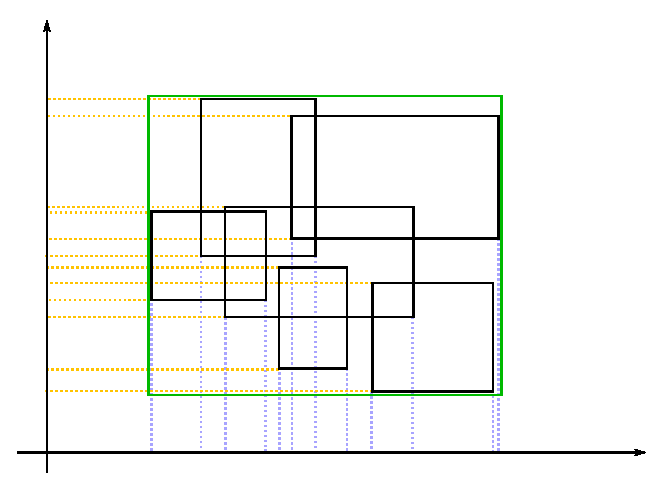
\includegraphics{img/04_rectangles.pdf}
    \caption{A \emph{partition grid} $G_V$ is the smallest structure containing all coordinates of its parts}
  \end{center}
\end{figure}

Let $i \in \set{1,\ldots,n}$.
We let $J_i = \set{\alpha_i^1, \beta_i^1, \alpha_i^2, \beta_i^2, \ldots, \alpha_i^k, \beta_i^k}$.
But this is unordered. Sort $J_i$ in ascending order
\[ J_i = \set{\xi_i^0, \xi_i^1, \ldots, \xi_i^{L_i}} \]
with $\xi_i^{l-1} < x_i^l$ for $l = 1, \ldots, l^i$.
Duplicate entries can be skipped.

$\forall j \in \set{1,\ldots,k}$, $\alpha_i^j$ and $\beta_i^j$ occurs among $\xi_i^l$.
This means that $\exists r_i^j, s_i^j \in \set{0, \ldots, L^i}: \alpha_i^j = \xi_1^{n_i^j}$ and $\beta_i^j = \xi_i^{s_i^j}$
because $\alpha_i^j < \beta_i^j \implies r_i^j < s_i^j$.
\[ G_v = \setdef{(\xi_i^{l_i})_{i=1}^n \in \mathbb R^n}{0 \leq l_i \leq L_i} \]
is called the \emph{partition grid of $V$}. Let
\[ \xi = (\xi_i^{l_i})_{i=1}^n \]
be a point of the partition grid
$l_1 \geq 1 \forall i \in \set{1,\ldots,n}$ (not zero, because otherwise there is no space for the cuboid left).

$\implies$ the cuboid at the left bottom of $\xi$:
\[ Q^{l_1 l_2 \ldots l_n} = Q^\xi = \bigtimes_{i=1}^n \left[\xi_i^{l_{i-1}}, \xi^{l_i}\right) \in \mathcal W \]
is called. Cuboid of partition grid of $V$.

% TODO insert graphics

\begin{lemma}
  \label{l:seven}
  Let $\xi = (\xi_i^{l_1})_{i=1}^n$ and $\xi' = (\xi_i^{l_i'})_{i=1}^n$ in $G_v$ with $\xi = \xi'$ (hence, at least one coordinate is different)
  \begin{itemize}
    \item $Q^\xi \cap Q^{\xi'} = \emptyset$ and $l_i, l'_i \geq 1$
    \item Let $j \in [1,\ldots,k]$. $\implies \forall \xi \in G_v: l_i \geq 1: \not\left[Q_j^\xi \cap Q_j = \emptyset \land Q^\xi \subseteq Q_j\right]$
  \end{itemize}
\end{lemma}
\begin{proof}
  \begin{itemize}
    \item
      Let $\xi \neq \xi'$.
      \[ \exists i \in \set{1,\ldots,n}: l_i \neq l_i' \]
      (The enumeration is different.) Assuming $x \in Q^\xi \land x \in Q^{\xi'}$
      \[ \implies x_i \in [\xi_i^{l_{i-1}}, \xi_i^{l_i}) \land x_i \in [\xi_i^{l'_{i-1}}, \xi_i^{l_i}) \]
      A visualization is given in Figure~\ref{img:lemma7a}.
      \[ \implies [\xi_i^{l_{i-1}}, \xi_i^{l_i}) \cap [\xi_i^{l'_{i-1}}, \xi_i^{l'_i}) \neq \emptyset \]
      for $l_i \neq l'_i$. This is a contradiction.
    \item
      Let $Q^\xi \cap Q_j \neq \emptyset$. Show that $Q^\xi \subseteq Q_j$.
      Let $x \in Q^\xi \cap Q_j$.
      \[ \implies \forall i: x_i \in [\xi_{i}^{l_{i-1}}, \xi_i^{l_i}) \land x_i \in [\alpha_i^j, \beta_i^j) \]
      where $[\alpha_i^j, \beta_i^j) = [\xi_i^{r_i^j}, \xi_i^{s_i^j})$ with $r_i^j \leq l_{i-1} < l_i \leq s_i^j$.
      \[ \implies [\xi_i^{l_{i-1}}, \xi_i^{l_i}] \subseteq [\alpha_i^j, \beta_i^j] \]
      \[ \implies Q^\xi = \bigtimes_{i=1}^{n} [\xi_i^{l_i}, \xi_i^{l_i}) \subseteq \bigtimes_{i=1}^n [\alpha_i^j, \beta_i^j) = Q^j \]
  \end{itemize}
\end{proof}

\begin{figure}[!h]
  \begin{center}
    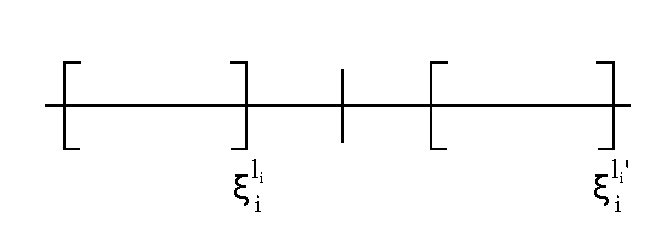
\includegraphics{img/07_lemma_7.pdf}
    \caption{Lemma 7 construction, item 1}
    \label{img:lemma7a}
  \end{center}
\end{figure}

\begin{lemma}
  \label{l:eight}
  Let $V = \bigcup_{j=1}^{k} Q_j \in R_W$.
  \[ \implies V = \bigcup_{\substack{\xi \in G_V, \xi_i \geq 1 \\ \text{and } Q_j \cap V \neq \emptyset}} Q^\xi \]
  Hence, we wrap all cuboids of the partition grid (which are disjoint!)
  which have at least one point with $V$ in common resulting precisely in $V$.
\end{lemma}
\begin{proof}
  \[ V' = \bigcup_{\substack{\xi \in G_V, \xi_i \geq 1 \\ \text{and } Q_j \cap V \neq \emptyset}} Q^\xi \]
  Show that $V' = V$.

  First, we prove the relation $\subseteq$. \\
  Let $x \in Q^\xi: Q^\xi \cap V \neq \emptyset$.
  \[ \implies \exists j \in [1,\ldots,k]: Q_j \cap Q^\xi \neq \emptyset \]
  By Lemma~7,
  \[ \implies Q^\xi \subseteq Q_j \]
  \[ \implies x \in Q_j \subseteq V \]
  \[ \implies x \in V \]

  Second, we prove the relation $\supseteq$. \\
  Let $x \in V$.
  \[ \exists j \in \set{1,\ldots,k}: x \in \theta_j = [\xi_i^{r_i^j}, \xi_i^{s_i^j}) \text{ with } r_i^j < s_i^j \]
  \[ \exists l_i: r_i^j \leq l_i - 1 < l_i \leq s_i^j \text{ with } x_i \in [\xi_{i}^{l_{i-1}}, \xi_i^{l_i}) \]

  \begin{figure}[!h]
    \begin{center}
      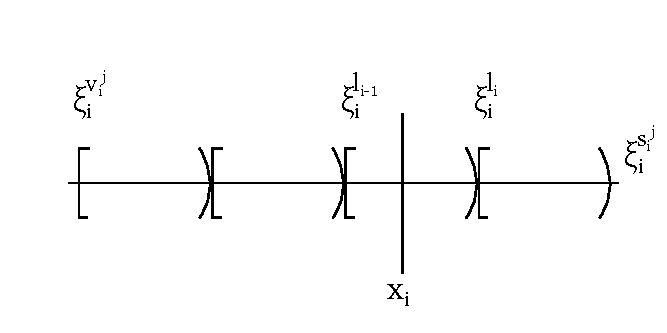
\includegraphics{img/08_lemma8.pdf}
      \caption{Lemma 8}
    \end{center}
  \end{figure}

  \[ \implies x \in \bigtimes_{i=1}^{n} [\xi_i^{l_{i-1}}, \xi_i^{l_i}) = Q^\xi \cap \set{x} \subseteq Q^\xi \cap Q_j \]
  \[ \implies Q^\xi \land V \neq \emptyset \]
  \[ \implies x \in V' \]
\end{proof}


%\dateref{2017/10/11}
% TODO: what? we already had 2017/10/13 and this example is too short for one lecture
%   Update, I think this dateref is just trailing

\begin{example}
  \[ Q \coloneqq X_{i=1}^n [\alpha_i, \beta_i) \qquad \text{cuboid} \qquad \alpha_1 \geq \beta_1 \text{ for some } i \implies Q = \emptyset \]
  \[ W = \setdef{Q \subseteq \mathbb R^n}{Q = X_{i=1}^n [\alpha_i, \beta_i)} \]
  \[ R_W = \setdef{V = \bigcup_{j=1}^m Q_j}{m \in \mathbb N \land Q_j \in W \text{ for } j = 1,\ldots,m} \]
\end{example}

\dateref{2017/10/18}
\section{Definition of measure}
\[ \mathcal R: \sigma\text{-ring} \]
\[
    \mu: \mathcal R \mapsto [0, \infty];
    \mu(\varphi) = 0,
    \sum_{n=1}^\infty \mu(A_n) = \mu(\bigcup_{n=1}^\infty A_n) \forall A_n \in \mathcal R \text{ and } A_n \cap A_m = \varphi \text{ for } n \neq m
\]
$\mu$ is measure on $\mathcal R$ (usually $\mathcal R = \mathcal A$ is a $\sigma$-algebra).
\[ A, B \in \mathcal R, A \subseteq B \implies \mu(A) \leq \mu(B) \qquad \text{monotonicity} \]
If $A \subseteq B$ and $\mu(B) < \infty$, then $\mu(A) = \mu(B) - \mu(B \setminus A)$
because of additivity: $\mu(A) + \underline{\mu(B \setminus A)}_{< \infty} = \underline{\mu(B)}_{< \infty} \implies \mu(A) = \mu(B) - \mu(B \setminus A)$.

\begin{lemma}
  \label{l:nine}
  \begin{enumerate}
    \item
      Let $\mathcal R$ be a $\sigma$-ring, let $\mu$ be a measure on $\mathcal R$ $(A_n)_{n \in \mathbb N}$, $A_n \in \mathcal R$.
      $A_n$ is ascending (dt. \enquote{aufsteigend}), i.e., $A_n \subseteq A_{n+1}$. Then $A = \bigcup_{n=1}^\infty A_n \in \mathcal R$
      and $\mu(A) = \mu\left(\bigcup_{n=1}^\infty A_n\right) = \lim_{n \to \infty} \mu(A_n)$
      and $A_n \cap A_m = \varphi$ for $n \neq m$.
    \item
      Let $A_n \in \mathcal R$, $A_{n+1} \subseteq A_n \forall n \in \mathbb N$ be a descending sequence
      and we assume that $\exists n' \in \mathbb N$: $\mu(A_{n'}) < \infty$.
      Then $A = \bigcap_{n=1}^\infty A_n \in \mathbb R$ and $\mu(A) = \mu(\bigcap_{n=1}^\infty A_n) = \lim_{n\to\infty} \mu(A_n)$.
  \end{enumerate}
\end{lemma}

How can the intersection be zero, if the sequence is descending?
Well, one example is $A_n = (n, \infty)$. The intersection is certainly zero, but each individual element has an infinite measure.

\begin{proof}
  \begin{enumerate}
    \item
      We build a sequence $B$ which represents the difference between consecutive elements of $A$.

      $B_1 = A_1, B_n = A_n \setminus A_{n-1}$ for $n \geq 2$, $B_n \in \mathcal R$.
      $B_n \cap B_m = \emptyset$ for $n \neq m$. Suppose $n \neq m$ without loss of generality $m > n$.
      Let $x \in B_n \cap B_m$. Then $x \in A_m$ but $x \not\in \underbrace{A_{m-1}}_{\geq n}$.
      $x \not\in A_n$ because $A_n \subseteq A_{m-1}$. $\implies x \not\in B_n \subseteq A_n$.

      $A_n = \bigcup_{k=1}^n B_k$ because
      \[ \bigcup_{k=1}^n B_k = \bigcup_{k=1}^n \left(A_k \setminus A_{k-1}\right) = \bigcup_{k=1}^n A_k \setminus \underbrace{\bigcap_{k=0}^{n-1} A_k}_{= \emptyset} = \bigcup_{k=1}^n A_k = A_n \]

      \[ \bigcup_{n=1}^\infty A_n = \bigcup_{n=1}^\infty \bigcup_{k=1}^n B_k = \bigcup_{n=1}^\infty B_n \]
      By $\sigma$-additivity it follows that
      \begin{align*}
        \mu\left(\bigcup_{n=1}^\infty A_n\right)
          &= \mu\left(\bigcup_{n=1}^\infty B_n\right) = \sum_{n=1}^\infty \mu(B_n) = \lim_{n\to\infty} \sum_{k=1}^n \mu(B_k) \\
          &= \lim_{n\to\infty} \mu\left(\overbrace{\bigcup_{k=1}^n B_k}^{= A_n}\right) = \lim_{n\to\infty} \mu(A_n)
      \end{align*}

    \item
      $A_{n+1} \subseteq A_n$. Without loss of generality, $n' = 1$, i.e., $\mu(A_n) < \infty$.
      $C_k = A_1 \subseteq A_k \subseteq A \setminus A_{k+1} = C_{k+1}$.
      $(C_k)^\infty_{k=1}$ is ascending.
      In that sense, $C_3$ covers the area of $A_1$ and $A_2$ but without the area of $A_3$ (which contains the subsequent elements $A_4$, $A_5$, \dots).
      \begin{align*}
        \bigcup_{n=1}^\infty C_n
            &= \bigcup_{n=1}^\infty \left(A_1 \setminus A_n\right) = A_1 \setminus \bigcap_{n=1}^\infty A_n \\
        \intertext{Take $\mu$ on both sides}
            &\overbrace{=}^{\text{due to part 1 of the proof}} \mu\left(\bigcup_{n=1}^\infty C_n\right) = \mu\left(A_1 \setminus \bigcap_{n=1}^\infty A_n\right) \\
            &\overbrace{=}^{\text{because } \mu(A_1) < \infty} \mu(A_1) - \mu(\bigcap_{n=1}^\infty A_n)
            &= - \mu(\bigcap_{n=1}^\infty A_n) \\
        \lim_{n\to\infty} (\mu(A_1) - \mu(A_n)) &= \mu(A_1) - \lim_{n\to\infty} \mu(A_n) \\
            &= -\mu(\bigcap_{n=1}^\infty A_n)
      \end{align*}
      \[ \implies \mu(\bigcap_{n=1}^\infty A_n) = \lim_{n\to\infty} \mu(A_n) \]

      Appendum: If $\mathcal R$ is a ring and $A, B \in \mathcal R$.
      \[ \Rightarrow A \cap B = \underbrace{A \setminus \underbrace{(A \setminus B)}_{\in \mathcal R}}_{\in \mathcal R} \]
      If $\mathcal R$ is a $\sigma$-ring, $A_n \in \mathcal R$, then $\bigcap_{n=1}^\infty A_n \in \mathcal R$.

      In other words:
      $\sigma$-ring $\mathcal R$ is closed with respect to countable intersection.
      A ring is closed with respect to finite intersection.
  \end{enumerate}
\end{proof}

\subsection{A method for generating $\sigma$-algebras}

\begin{lemma}
  \label{l:ten}
  Suppose we have a non-empty set $X \neq \emptyset$. Let $(\mathcal A_i)_{i \in I}$ be a family of $\sigma$-algebra on $X$.
  Then $\mathcal A = \bigcap_{i \in I} \mathcal A_i \neq \emptyset$ is a $\sigma$-algebra on $X$.
\end{lemma}

\begin{proof}
  Let $x \in \mathcal A_i \forall i \in I$. Then $x \in \bigcap_{i \in I} \mathcal A_i = A$ likewise $\varphi \in \mathcal A$.

  We need to show that $A \in \mathcal A \implies A^C \in \mathcal A$.

  Let $A \in \mathcal A$, i. e., $\forall i \in I: A \in \mathcal A_i$.
  Because $\mathcal A_i$ is a $\sigma$-algebra $A^C \in \mathcal A_i \forall i \in I \implies A^C \in \mathcal A = \bigcap_{i \in I} A_i$.

  We need to show that $A_n \in \mathcal A \forall n \in \mathbb N$. Then $\bigcup_{n=1}^\infty A_n \in \mathcal A$.
  Assume $\forall n \in \mathbb N: A_n \in \mathcal A$, i.e., $A_n \in \mathcal A_i \forall i \in I$.
  That means $\bigcup_{n=1}^\infty A_n \in \mathcal A_i \forall i \in i$. $\implies \bigcup_{n=1}^\infty A_n \in \mathcal A$.
\end{proof}

\begin{definition}
  Let $X \neq \emptyset$. $M \subseteq \mathcal P(X)$ (where $\mathcal P$ denotes the power set).
  We set
  \[ \mathcal A_m = \bigcap_{\substack{M \subseteq \mathcal A \subseteq \mathcal P(X) \\ \mathcal{A} \text{ is a } \sigma\text{-algebra}}} \mathcal A \]
  Then $A_m$ is a $\sigma$-algebra, $A_m$ is not empty, because $\mathcal A = \mathcal P(X)$ is a $\sigma$-algebra which contains $M$.

  We call $\mathcal A_m$ the $\sigma$-algebra generated by $M$.
  $A_m$ is the smallest $\sigma$-algebra that contains $M$. This means that for every $\sigma$-algebra $\mathcal A$ with $M \subseteq \mathcal A$, we have $\mathcal A_m \subseteq \mathcal A$.
\end{definition}

Special case: Let $X$ be a topological space and $\tau$ is the topology on $X$; $\tau \subseteq \mathcal P(X)$.
Then we call $\mathcal B = \mathcal A_{\tau}$ the \enquote{Borel $\sigma$-algebra on $X$}.

\person{Emile Borel (1871-1956)}

\begin{example}[Examples of measures]
  Let $X \neq \emptyset$. We set $\mathcal A = \mathcal P(X)$.
  We define
  \[
    \mu_{C}(A) = \begin{cases}
      n \in \mathbb N & \text{ if } A \text{ contains exactly $n$ elements} \\
      \infty & \text{ if } A \text{ has infinitely many elements}
    \end{cases}
  \]
  $\mu_C$ is called the \enquote{counting measure on $X$} and satisfies the properties of a measure.
\end{example}

\begin{proof}
  \begin{enumerate}
    \item
      $\mu_C(\emptyset) = 0$.
    \item
      Proving $\sigma$-additivity is left as an exercise to the reader.
  \end{enumerate}
\end{proof}

\begin{example}
  Let $X \neq \emptyset$ and let $x \in X$ be fixed. We define
  \[ \mu_x(A) = \begin{cases} 1 & \text{ if } x \in A \\ 0 & \text{ if } x \not\in A \end{cases} \]
  We call $\mu_{x}$ a point-measure concentrated in $x$.
\end{example}

\begin{proof}
  We need to prove two statements:
  \begin{enumerate}
    \item \[ \mu_x(A) \geq 0 \qquad \mu_x(\emptyset) = 0 \]
    \item Let $(A_n)_{n \in \mathbb N}$ be pointwise disjoint.
  \end{enumerate}

  We prove the first statement:

  Case 1: $\exists n' \in \mathbb N$ with $x \in A_{n'}$ then $x \in \bigcup_{n=1}^\infty A_n$ and $\mu_x(\bigcup_{n=1}^\infty A_n) = 1 \forall n \neq n'$:
  $x \not\in A_n$ because otherwise $A_n \bigcap A_{n'} \neq \emptyset$. Therefore
  $\sum_{n=1}^\infty \mu_x(A_n) = \underbrace{\mu_{x}\left(A_{n'}\right)}_{=1} + \sum_{\substack{n = 1 \\ n \neq n'}}^\infty \underbrace{\mu_x(A_n)}_{=0} = 1$
  
  Case 2: $\forall n \in \mathbb N: x \not\in A_n \forall n \in \mathbb N$
  \[ \implies x \not\in \bigcup_{n=1}^\infty A_n \land \mu_X(\bigcup_{n=1}^\infty A_n) = 0 \]
  And also,
  \[ \sum_{n=1}^\infty \underbrace{\mu_x(A_n)}_{=0} = 0 \]

  \begin{lemma}[Lemma 11]
    Let $\mathcal R$ be a $\sigma$-ring.
    $A_n \in \mathcal R$ for $n = 1, 2, 3, \ldots$ and $\mu: \mathcal R \mapsto [0,\infty]$ be a measure.
    Then
    \[ \mu\left(\bigcup_{n=1}^\infty A_n\right) \leq \sum_{n=1}^\infty \mu(A_n) \]
    This property is called \enquote{sub-additivity}.
  \end{lemma}

  \begin{definition}
    Let $X \neq \emptyset$. $\mu^*: \mathcal P(X) \mapsto [0, \infty]$.
    Then $\mu^*$ is called \enquote{outer measure on $X$} if
    \begin{itemize}
      \item $\mu^*(\varphi) = 0$
      \item $A \subseteq B \implies \mu^*(A) \leq \mu^*(B)$ (monotonicity)
      \item $A_n \subset X$ for $n = 1, 2, \ldots$. $\mu^*(\bigcup_{n=1}^\infty A_n) \leq \sum_{n=1}^\infty \mu^*(A_n)$ (sub-additivity)
    \end{itemize}
  \end{definition}
\end{proof}

\dateref{2017/10/20}

TODO

\dateref{2017/10/25}

$\mu^*$ is an outer measure on $X$.
\[ M_{\mu^*} = \set{A \subseteq X: A \text{ is } \mu^* \text{ measurable}} \]
$A$ is measurable iff $\forall Y \subseteq X: \mu^*(Y) = \mu^*(Y \cap A) + \mu^*(Y \setminus A) = \mu^*(Y \cap A) + \mu^*(Y \cap A^C)$


\begin{theorem}[Theorem 1]
  Let $\mu^*$ be an outer measure on $X \neq \mu$.
  Let $M_{\mu^*}$ be the set of all measurable subsets of $X$.
  Then
  \begin{enumerate}
    \item $M_{\mu^*}$ is a $\sigma$-algebra.
    \item $\left.\mu^*\right|_{M_{\mu^*}}$ is a measure.
  \end{enumerate}
\end{theorem}

This construction (to build a measure from an outer measure) is due to Constantin Caratheodory.

\begin{proof}
  We need to prove:
  \begin{enumerate}
    \item Let $A \in M_{\mu^*} \implies A^C \in M_{\mu^*}$.
    \item Let $X \in M_{\mu^*}$, $\varphi \in M_{\mu^*}$.
    \item $(A_n)_{n \in \mathbb N}$, $A_n \in M_{\mu^*} \implies \bigcup_{n=1}^\infty A_n \in M_{\mu^*}$
  \end{enumerate}

  We first need to the auxiliary statement:
  \[ \forall B_n \in M_{\mu^*}: B_n \cap B_m = \emptyset \quad \forall m \neq n \]
  \[ \mu^*\left(\bigcup_{n=1}^{\infty} B_n\right) = \sum_{n=1}^\infty \mu^*(B_n) \]

  We prove the first assertion:
  \[ \forall Y \subseteq X \text{ and } \forall A \subseteq X \]
  \[ \mu^*(Y) \underbrace{\leq}_{\text{sub additivity}} \mu^*(Y \cap A) + \mu^*(Y \subseteq A) \]
  because $Y = (Y \cap A) \cup (Y \setminus A)$.
  Let $A$ be measurable, show that $A^C \in M_{\mu^*}$. Choose $Y \subseteq X$ arbitrary.
  \begin{align*}
    \mu^*(Y \cap A^C) + \mu^*(Y \setminus A^C)
      &= \mu^*(Y \cap A^C) + \mu^*(Y \cap (A^C)^C) \\
      &= \mu^*(Y \cap A) + \mu^*(Y \cap A^C) \underbrace{=}_{A \in M_{\mu^*}} \mu^*(Y)
  \end{align*}
  \[ \mu^*(\underbrace{Y \cap \emptyset}_{\emptyset}) + \mu^*(\underbrace{Y \setminus \emptyset}_{Y}) = \underbrace{\mu^*(\emptyset)}_{=0} + \mu^*(Y) = \mu^*(Y) \]

  So $\emptyset \in M_{\mu^*}$ and $X = (\emptyset)^C \in M_{\mu^*}$.
  We proved the second assertion.

  We prove the third assertion:
  Show: $A_1, A_2 \in M_{\mu^*}$ then $A_1 \cup A_2 \in M_{\mu^*}$.
  Let $Y \in X$ be chosen.
  \begin{align*}
    \mu^*(y)
      &\leq \mu^*(Y \setminus (A_1 \cup A_2)) + \mu^*(Y \cap (A_1 \cup A_2)) \\
      &= \mu^*((Y \setminus A_1) \setminus A_2) + \mu^*((Y \cap A_1) \cup (Y \setminus A_1) \cap A_2) \\
      &\stackrel{\leq}{\text{sub-additivity}} \mu^*((Y \setminus A_1) \setminus A_2) + \mu^*((Y \setminus A_1) \cap A_2) + \mu^*(Y \cap A_1) \\
      &\stackrel{=}{\substack{A_2 \in M_{\mu^*} \\ Y \setminus A_1 \text{ as testset}}} \mu^*(Y \setminus A_1) + \mu^*(Y \cap A_1) \stackrel{=}{A_1 \text{ is measurable}} \mu^*(Y)
  \end{align*}
  So, all \enquote{$\leq$} are \enquote{$=$}.

  \[ \mu^*(Y) = \mu^*(Y \cap (A_1 \cup A_2)) + \mu^*(Y \setminus (A_1 \cup A_2)) \implies A_1 \cup A_2 \in M_{\mu^*} \]
  By induction, $A_1, \ldots, A_v \in M_{\mu^*} \implies \bigcup_{n=1}^N A_n \in M_{\mu^*}$.

  Now we want prove the auxiliary statement:
  Let $B_1, \ldots, B_N \in M_{\mu^*}$, $B_n \cap B_m = \emptyset$ for $n\neq m$.
  Then $\mu^*\left(\bigcup_{n=1}^N B_n\right) = \sum_{n=1}^N \mu^*(B_n)$.
  We prove this by induction.
  Let $N=2$.
  \begin{align*}
    \mu^*(B_1 \cup B_2) &\underbrace{=}_{B_2 \in M_{\mu^*}} \mu^*((B_1 \cup B_2) \cap B_2) + \mu^*((B_1 \cup B_2) \setminus B_2) \\
        &\underbrace{=}{B_1 \cap B_2 = \emptyset} \mu^*(B_2) + \mu^*(B_1)
  \end{align*}
  The general induction step is left as an exercise to the reader.

  Let $(B_n)_{n=1}^\infty$ be measurable. $B_n \cap B_m = \emptyset$.
  \begin{align*}
    \mu^*(\bigcup_{n=1}^\infty B_n) 
      &\stackrel{\leq}{\text{sub-additivity}} \sum_{n=1}^\infty \mu^*(B_n) \\
      &= \lim_{N\to\infty} \sum_{n=1}^N \mu^*(B_n) \\
      &= \lim_{N\to\infty} \mu^*(\bigcup_{n=1}^N B_n) \\
      &\stackrel{\leq}{\text{monotonicity}} \lim_{N\to\infty} \mu^*(\bigcup_{n=1}^\infty B_n)
  \end{align*}
  So, all \enquote{$\leq$} are \enquote{$=$}. So,
  \[ \mu^*(\bigcup_{n=1}^\infty B_n) = \sum_{n=1}^\infty \mu^*(B_n) = \mu^*(\bigcup_{n=1}^\infty B_n) \]
  $B_n \cap B_m \neq \emptyset$ for $B_n \in M_{\mu^*}$.
\end{proof}

Let $(A_n)_{n=1}^\infty$ and $A_n \in M_{\mu^*}$.
Check that $\bigcup_{n=1}^\infty A_n$ satisfies the measurability condition.
\[ B_1 = A_1 \qquad B_n = A_n \setminus \bigcup_{k=1}^{n-1} A_k \]
Then $B_n \cap B_m = \emptyset$ for $m \neq n$.

Check, whether $\bigcup_{n=1}^\infty B_n$ satisfies the measurability condition.
\[ C_n = \bigcup_{n=1}^N B_n, \quad C_n \in M_{\mu^*}, \quad \quad C = \bigcup_{n=1}^\infty B_n \]
Let $Y \subseteq X$ be chosen arbitrarily.

\begin{claim}
  \[ \mu^*(Y \cap C_N) = \sum_{n=1}^N \mu^*(Y \cap B_n) \]
\end{claim}
\begin{proof}
  Proof by induction:
  $N=1$ follows immediately. We prove $N \to N+1$:
  \begin{align*}
    \mu^*(Y \cap C_{N+1})
      &\stackrel{\substack{B_{N+1} \text{ is } \\ \text{measurable}}}{=} \mu^*((Y \cap C_{N+1}) \cap B_{N+1}) + \mu^*((Y \cap C_{N+1}) \setminus B_{N+1}) \\
      &= \mu^*(Y \cap B_{N+1}) + \mu^*(Y \cap C_N) \\
      &\stackrel{\substack{\text{induction} \\ \text{hypothesis}}}{=} \mu^*(Y \cap B_{N+1}) + \sum_{n=1}^N \mu^*(Y \cap B_n) \\
      &= \sum_{n=1}^{N+1} \mu^*(Y \cap B_n)
  \end{align*}
  % TODO: check the following line
  \[ \sum_{n=1}^N \mu^*(Y \cap B_n) + \mu^*(Y \setminus C) = \mu^*(Y \cap C_N) + \mu^*(Y \setminus C) \stackrel{\text{monotonicity}}{\leq} \mu^*(Y \cap C_N) + \mu^*(Y \setminus C_N) = \mu^*(Y) \]
  Recall that $C_N$ are finite unions in $M_{\mu^*}$.

  \[ N \to \infty \implies \sum_{n=1}^\infty \mu^*(Y \cap B_n) + \mu^*(Y \setminus C) \leq \mu^*(Y) \]
  \begin{align*}
    \mu^*(Y) &\stackrel{\leq}{\text{sub additivity}} \mu^*(Y \cap C) + \mu^*(Y \setminus C) \\
      &= \mu^*(Y \cap \bigcup_{n=1}^\infty B_n) + \mu^*(Y \setminus C) \\
      &= \mu^*(\bigcup_{n=1}^\infty(Y \cap B_n)) + \mu^*(Y \setminus C) \\
      &\stackrel{\leq}{\text{sub additivity}} \sum_{n=1}^\infty \mu^*(Y \cap B_n) + \mu^*(Y \setminus C) \leq \mu^*(Y)
  \end{align*}

  Again: Every $\leq$ is an equality $=$.
  \[ \mu^*(Y) = \mu^*(Y \cap C) + \mu^*(Y \setminus C) \]
  So, $C = \bigcup_{n=1}^\infty B_n = \bigcup_{n=1}^\infty A_n \in M_{\mu^*}$.
\end{proof}

\[ \lambda^*(A) = \int_{\substack{(Q_j)^n_{j=1}, Q_j \in W \\ A \subseteq \bigcup_{j=1}^\infty Q_j}} \sum_{j=1}^\infty \operatorname{vol}_n(Q_j) \]
$\lambda^*$ is an outer measure on $\mathbb R^n$.

We still need to check whether $\lambda^*$ is monotone.
Let $A \subseteq B \subseteq \mathbb R^n$.
Consider a covering $(Q_j)_{j=1}^\infty$, $Q_j \in W$ with $B \subseteq \bigcup_{j=1}^\infty Q_j$.
Obviously $A \subseteq \bigcup_{j=1}^\infty Q_j$.
So $(Q_j)_{j=1}^\infty$ covers $A$.

\begin{align*}
  \mu^*(A)
    &= \underbrace{\inf_{\substack{Q'_j \in W \\ A \subseteq \bigcup_{j=1}^\infty {Q'}_{j'}}} TODO}_{\text{larger set}}
      \sum_{j=1}^\infty \operatorname{vol}_n(Q'_j) \\
    &\leq \inf_{\underbrace{\substack{Q_j \in W \\ B \subseteq \bigcup_{j=1}^\infty TODO}}_{\text{smaller set}}}
      \sum_{j=1}^\infty \operatorname{vol}_n(Q_j)  \\
    &= \lambda^*(B) \text{ so } \lambda^* \text{ is monotone}
\end{align*}

\index{Null set}
\index{Zero set}
\begin{definition}
  Let $\mu^*$ be an outer measure on $P(X)$.
  We call $N \subseteq X$ with $\mu^*(N) = 0$ a \emph{null set} (also called \enquote{zero set}).
\end{definition}

\index{complete measure space}
Let $(X, A, \mu)$ be a measure space. We call $N \in A$ a null set if $\mu(N) = 0$.
A measure space ($X, A, \mu$) is called \emph{complete} if for all null sets $N \in A$
and any $N' \subseteq N$ we have $N' \in A$ (and $\mu(N') = 0$).

\begin{lemma}[Lemma 13]
  Let $\mu^*$ be an outer measure. $N \subseteq X$ with $\mu^*(N) = 0$.
  Then $N \in M_{\mu^*} \implies N$ is null set in ($X, M_{\mu^*}, \mu$).
  This means that ($X, M_{\mu^*}, \mu$) is complete.
\end{lemma}
\begin{proof}
  Let $N$ be a $\mu^*$-nullset, $Y \subseteq X$ be chosen.
  \[
      \mu^*(Y)
        \leq \mu^*(\underbrace{Y \cap N}_{\subseteq N}) + \mu^*(\underbrace{Y \setminus N}_{\subseteq Y})
        \stackrel{\leq}{\text{monotonicity}} \underbrace{\mu^*(N)}_{=0} + \mu^*(Y) = \mu^*(Y)
  \]
  Again, we get $=$ instead of $\leq$.

  $N \in M_{\mu^*}$:
  Now let $N \subset X$ be a $\mu^*$-nullset (also a ($X, M_{\mu^*}, \mu$)-nullset)
  and $N' \subseteq N$, $\mu^*$ is monotone
  $\implies \mu^*(N') = 0 \implies N' \in M_{\mu^*}$.
\end{proof}

\dateref{2017/10/27}

\[ \forall Q \in W \implies Q \in M_{X^*}, \lambda^*(Q) = \lambda(Q) = \operatorname{vol}_n(Q) \]

\begin{definition}
  Let $X = \mathbb R^n$ and $\lambda^*$ is an outer Lebesgue measure on $\mathbb R^n$.
  We set $\mathcal L = M_{\lambda^*}$ as $\sigma$-algebra of Lebesgue measureable sets in $\mathbb R^n$.
  \[ A \in \mathcal L \Leftrightarrow \forall Y \subseteq \mathbb R^n: \lambda^*(Y) = \lambda^*(Y \cap A) + \lambda^*(Y \setminus A) \]
  $\left.\lambda^*\right|_{\mathcal L} = \lambda$ is the Lebesgue measure on $\mathbb R^n$.
\end{definition}

\begin{lemma}[Lemma 14]
  Let $Q \in W$. $Q = X_{x=1}^n [\alpha_i, \beta_i)$ and $\alpha_i \leq \beta_i$.
  Let $\xi_1^0 = \alpha_1 \leq \xi_i^1 \leq \xi_i^2 \leq \ldots \leq \xi_i^{L_i} = \beta_i$ is a partition of $[\alpha_i, \beta_i)$.
  \[ G = \set{\begin{bmatrix} \xi_1^{l_1} \\ \vdots \\ \xi_n^{l_n} \end{bmatrix}; 0 \leq l_i \leq L_i} \]
  is a partition grid for $Q$.
  \[ G' = \set{\begin{bmatrix} \xi_1^{l_1} \\ \vdots \\ x_n^{l_n} \end{bmatrix}; 1 \leq l_i \leq L_i} \]
  For $\xi = \begin{bmatrix} \xi_1^{l_1} \\ \vdots \\ \xi_n^{l_n} \end{bmatrix} \in G'$ we set $Q^\xi = X_{i=1}^n [\xi_i^{l_1 - 1}, \xi_i^{l_1})$.

  \begin{figure}[t]
    \begin{center}
      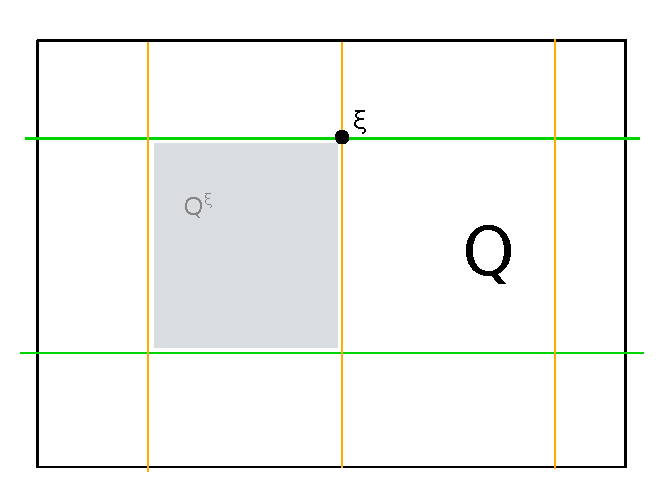
\includegraphics{img/09_lebesgue.pdf}
      \caption{Construction of Lemma 14}
    \end{center}
  \end{figure}

  Then $\operatorname{vol}_n(Q) = \sum_{\xi \in G'} \operatorname{vol}_n(Q^\xi)$.
\end{lemma}

\begin{proof}
  \begin{align*}
    \sum_{\xi \in G'} \operatorname{vol}_n(Q^\xi) &= \sum_{l_1=1}^{L_1} \sum_{l_2=1}^{L_2} \ldots \sum_{l_n=1}^{L_n} \pi_{i=1}^n \left(\xi_i^{l_i} - \xi_i^{l_i - 1}\right) \\
      &= \left[\sum_{l_1=1}^{L_1} (\xi_1^{l_1} - \xi_1^{l_1-1})\right] \underbrace{\left[\sum_{l_2=1}^{L_2} (\xi_2^{l_2} - \xi_2^{l_2-1})\right]}_{\text{telescoping sum}} \ldots \left[\sum_{l_n=1}^{L_n} (\xi_n^{l_n} - \xi_n^{l_n-1})\right] \\
      &= \prod_{i=1}^n (\xi_i^{L_i} - \xi_i^0) = \prod_{i=1}^n (\beta_i - \alpha_i) = \operatorname{vol}(Q)
  \end{align*}
\end{proof}

\begin{lemma}[Lemma 15]
  Let $Q \in W$, $Q = \bigcup_{j=1}^M Q_j$, $Q_j \in W$ and $Q_i \cap Q_l = \emptyset$ for $j=l$.
  Then $\operatorname{vol}_n(Q) = \sum_{j=1}^M \operatorname{vol}_n(Q_j)$.

  \begin{figure}[!h]
    \begin{center}
      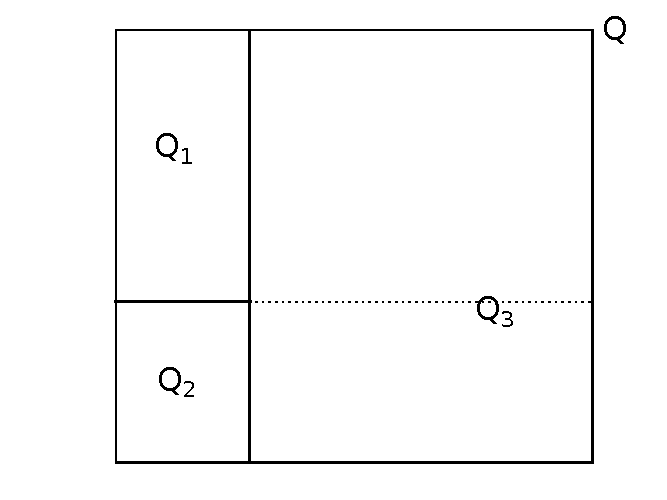
\includegraphics{img/10_lemma15.pdf}
      \caption{Construction of Lemma 15}
    \end{center}
  \end{figure}
\end{lemma}

\begin{proof}
  Let $G$ be the partitioning grid for the covering $(Q_j)_{j=1}^M$ of $Q$.
  \[ G' = \set{\begin{bmatrix}\xi_1^{l_1} \\ \vdots \\ \xi_n^{l_n} \end{bmatrix}; 1 \leq l_1 \leq L_i} \]
  $Q^\xi$ is above because $Q_j \subseteq Q$.
  \[ \alpha_1 \leq \xi_i^{l_1} \leq \beta_i \quad \forall i \in \set{1, \ldots, n}, l_i \in \set{0, \ldots, L_i} \]
  Let $x = \begin{bmatrix} x_1 \\ \vdots \\ x_n \end{bmatrix} \in Q$ then $x \in Q_j$ for some $j \in \set{1,\ldots,M}$.
  $x_i \in [\xi_1^{l_i-1}, \xi_1^{l_i})$ for exactly one $l_i \in \set{1,\ldots,L_i}$.
  Moreover: for the point $x = \begin{bmatrix} \alpha_1 \\ \vdots \\ \alpha_n \end{bmatrix} \in Q \implies \xi_i^0 = \alpha_i$ for all $i$.
  Also a point with $i-th$ coordinate $x_i = \beta_i - \varepsilon$ ($\varepsilon$ sufficiently small)
  which lies in $Q$ implies $\beta_i - \varepsilon < \xi_i^{L_i} \quad \forall \varepsilon > 0 \implies \beta_i \leq \xi_i^{L_i} \implies \beta_i = \xi_i^{L_i}$.

  The previous lemma stated that $\vol_n(Q) = \sum_{\xi \in G'} \vol_n(Q^\xi)$. And,
  \[ \sum_{j=1}^M \vol_n(Q_j) = \sum_{j=1}^M \sum_{\substack{\xi \in G' \\ Q^\xi \cap Q_j \neq \emptyset}} \vol_n(Q^\xi) = \sum_{\xi \in G'} \vol_n(Q^\xi) \]
  Hence, they are equal (because they have the same expression on the right-hand side).
\end{proof}

\begin{lemma}[Lemma 16, a sub-additivity result]
  Let $Q \in W$, $Q \subseteq \bigcup_{j=1}^M Q_j; Q_j \in W$.
  Then we have that $\vol_n(Q) \leq \sum_{j=1}^m \vol(Q_j)$.
  Now we cover $Q$ with a finite number of rectangle (possibly overlapping).
  \begin{figure}[!h]
    \begin{center}
      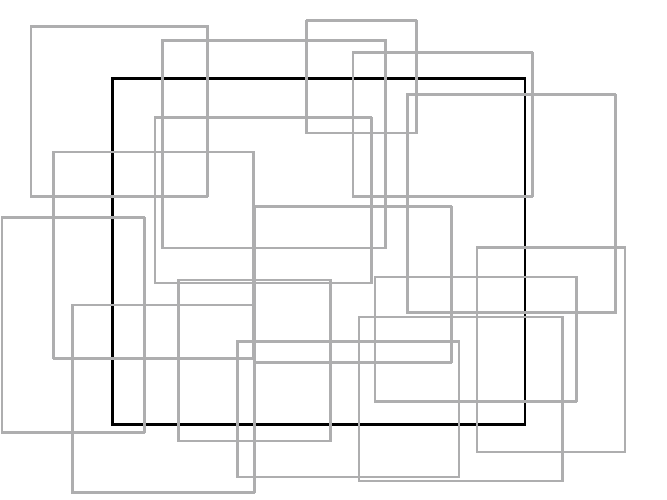
\includegraphics{img/11_lemma16.pdf}
      \caption{Lemma 16 construction}
    \end{center}
  \end{figure}
\end{lemma}

\begin{proof}
  We set $Q_0 = Q$ and construct the partitioning. Grid $G$ for $(Q_j)_{j=0}^M$.
  Let $\tilde Q \coloneqq \bigcup_{j=1}^M Q_j$.
  \[ Q \subseteq \bigcup_{j=0}^M Q_j = \bigcup_{j=1}^M Q_j = \bigcup_{\substack{\xi \in G' \\ Q^\xi \cap \tilde Q \neq \emptyset}} Q^\xi \]
  \begin{align*}
    Q &= \bigcup_{\substack{\xi \in G' \\ Q^\xi \cap Q \neq \emptyset}} Q^\xi \underbrace{\implies}_{\text{Lemma 15}} \vol_n(Q) \\
      &= \sum_{\substack{\xi \in G' \\ Q^\xi \cap Q \neq \emptyset}} \vol_n(Q^\xi) \\
      &\leq \sum_{\substack{\xi \in G' \\ Q^\xi \cap \tilde Q \neq \emptyset}} \vol_n(Q^\xi) \\
      &\leq \sum_{j=1}^M \sum_{\substack{\xi \in G' \\ Q^\xi \cap Q_j \neq \emptyset}} \vol_n(Q^\xi) \\
      &\underbrace{=}_{\text{Lemma 15}} \sum_{j=1}^M \vol_n(Q_j)
  \end{align*}
\end{proof}

\begin{lemma}[Lemma 17]
  Let $Q \in W$, $Q \subseteq \bigcup_{j=1}^\infty Q_j, Q_j \in W$.
  Then $\vol_n(Q) \leq \sum_{n=1}^{\infty} \vol_n(Q_j)$.
\end{lemma}

\begin{proof}
  Without loss of generality, $Q \neq \emptyset$ and $Q_j \neq \emptyset$.
  \[ \vol_n(Q) = \prod_{i=1}^n (\beta_i - \alpha_i) > 0 \qquad \vol_n(Q_j) > 0 \forall j \in \mathbb N \]
  Let $\vol_n(Q) > \varepsilon > 0$ be arbitrary (sufficiently small).
  We choose $Q_{\varepsilon} = X_{i=1}^n [\alpha_i^\varepsilon, \beta_i^\varepsilon) \subseteq \overline{Q}_\varepsilon = X_{i=1}^n [\alpha_i^\varepsilon, \beta_i^\varepsilon] \subseteq Q$ such that
  \[ \vol_n(Q_\varepsilon) = \vol_n(Q) - \varepsilon \]
  You will get this result if one lets,
  \[ \alpha_i^\varepsilon = \alpha_i + \frac12(\alpha_i - \beta_i)\left(1 - (1 - \frac{\varepsilon}{\vol_n(Q)})^\frac1n\right) \]

  Choose: $Q_j^\varepsilon \supseteq Q_j$, $Q_j^\varepsilon = X_{i=1}^n [\alpha_i^{j,\varepsilon}, \beta_i^{j,\varepsilon})$, $\alpha_i^{j,\varepsilon} < \alpha_i^j < \beta_i^j < \beta_i^{j,\varepsilon}$.
  \[ Q_j \subseteq \operatorname{int}(Q_j^\varepsilon) = Q_j^\varepsilon = X_{i=1}^n (\alpha_i^{j,\varepsilon}, \beta_i^{j,\varepsilon}) \text{ with } \vol(Q_j^\varepsilon) = \vol(Q_j) + \frac{\varepsilon}{2^j} \]
  Then
  \[
    Q_\varepsilon \subseteq Q \subseteq \bigcup_{j=1}^\infty Q_j \subseteq \bigcup_{j=1}^\infty Q_j^\varepsilon
    \underbrace{\implies}_{\text{compactness}} \exists M \subseteq N: \overline{Q}_\varepsilon \subseteq \bigcup_{j=1}^M Q_j
  \]
  $Q_\varepsilon$ is a bounded, closed set (hence, a compact set). Therefore, this result.
  \[ Q_3 \subseteq \overline{Q_3} \subseteq \bigcup_{j=1}^M Q_j^\varepsilon \subseteq \bigcup_{j=1}^M Q_j^\varepsilon \]
  \[ \underbrace{\implies}_{\text{Lemma 16}} \vol_n(Q_\varepsilon) \leq \sum_{n=1}^M \vol_n(Q_j^\varepsilon) = \sum_{j=1}^M \left(\vol_n(Q_j) + \frac{\varepsilon}{2^j}\right) \]
  \[ \leq \sum_{j=1}^\infty \vol_n(Q_j) + \varepsilon \cdot \underbrace{\sum_{j=1}^\infty \frac{1}{2^j}}_{=1} \]
  \[ \Leftrightarrow \vol_n(Q) \leq \sum_{j=1}^{\infty} \vol_n(Q_j) + 2\varepsilon \qquad \forall \varepsilon > 0 \]
  \[ \Leftrightarrow \vol_n(Q) \leq \sum_{j=1}^\infty \vol_n(Q_j) \]
\end{proof}

\begin{lemma}[Lemma 18]
  $\forall Q \in W$ we have $\vol_n(Q) = \lambda^*(Q)$.
\end{lemma}
\begin{proof}
  \[ \lambda^*(Q) = \inf_{\substack{Q \subseteq \bigcup_{j=1}^\infty Q_j \\ Q_j \in W}} \sum_{j=1}^\infty \vol_n(Q_j) \]
  $Q$ is a covering of $Q$, hence $\lambda^*(Q) \leq \vol_n(Q)$.
  On the other hand, because of Lemma~17, it follows that $\vol_n(Q) \leq \sum_{j=1}^\infty \vol_n(Q_j)$.
  For any covering $(Q_j)_{j=1}^\infty$ of $Q$ implies that
  \[ \vol_n(Q) \leq \inf_{Q \subseteq Q_{j=1}^\infty Q_j} \sum_{j=1}^\infty \vol_n(Q_j) = \lambda^*(Q) \]
  So $\lambda^*(Q) = \vol_n(Q)$.
\end{proof}

\begin{lemma}[Lemma 19]
  We have $W \subseteq \mathcal L$, i.e., every $Q \in W$ is measurable.
\end{lemma}
\begin{proof}
  Let $A \subseteq \mathbb R^n$ be given.
  Let $A \subseteq \bigcup_{j=1}^\infty Q_j$, $Q_j \in W$.
  \[ A \cap Q \subseteq \left(\bigcup_{j=1}^\infty Q_j\right) \cap Q = \bigcup_{j=1}^\infty \overbrace{(Q_j \cap Q)}^{\in W} \]
  \[ A \setminus Q \subseteq \bigcup_{j=1}^\infty (\underbrace{Q_j \setminus Q}_{\in \mathcal R_W}) \underbrace{\text{Lemma 6}} \bigcup_{j=1}^\infty \bigcup_{l=1}^{m_j} Q_l^j \]
  So $Q_j = (\underbrace{Q_j \cap Q}_{\in W}) \cup (\underbrace{\bigcup_{l=1}^{m_j} Q_l^j}_{\in W})$ disjoint union
  \[ \underbrace{\implies}_{\text{Lemma 15}} \vol_n(Q_j) = \vol(Q \cap Q_j) + \sum_{l=1}^{m_j} \vol(Q_l^j) \]
  \[ \sum_{j=1}^\infty \vol(Q_j) = \sum_{j=1}^\infty \vol(\underbrace{Q \cap Q_j}_{\text{cover } Q \cap A}) + \sum_{j=1}^\infty \sum_{l=1}^{m_j} \vol(\underbrace{Q_l^j}_{\text{cover } A \setminus Q}) \]
  \[ \geq \lambda^*(Q \cap A) + \lambda^*(A \setminus Q) \]
  holds for every covering $(Q_j)_{j=1}^\infty$ of $A$.
  Taking \enquote{inf} implies that
  \[ \lambda^*(A) \geq \lambda^*(Q \cap A) + \lambda^*(A \setminus Q) \]
  \[ \lambda^*(A) \leq \lambda^*(Q \cap A) + \lambda^*(A \setminus Q) \]
  \[ \vol_n(Q_j) = \vol(Q \cap Q_j) + \sum_{l=1}^{m_j} \vol(Q_l^j) \]
  Due to sub-additivity,
  \[ \lambda^*(A) = \lambda^*(A \cap Q) + \lambda^*(A \setminus Q) \]
  so $Q \in \mathcal L$.
\end{proof}

\dateref{2017/11/08}

\[ \lambda(Q) = \vol_n(Q) \]
We let $\underbrace{Q(x, r)}_{\in W} = \times_{i=1}^n [x_i - r_, x_i + r)$ for $x = (x_1, \ldots, x_n)^t \in \mathbb R$ and $r > 0$.

\begin{figure}[!h]
  \begin{center}
    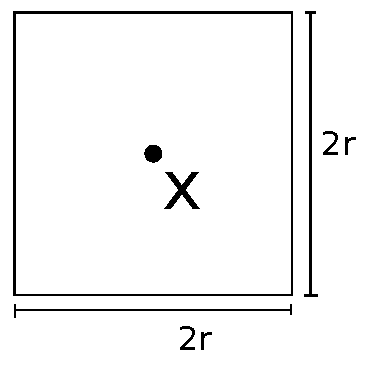
\includegraphics{img/13_q.pdf}
    \caption{$Q$ for Lemma 20}
  \end{center}
\end{figure}

\begin{lemma}[Lemma 20]
  Let $x \in \mathbb R^n$, $r>0$. Then $B(x,r) \subseteq Q(x,r) \subseteq B(x, \sqrt{n} r + \varepsilon) \forall \varepsilon > 0$.
\end{lemma}
\begin{proof}
  Let $y \in B(x,r)$, i.e., $\|x - y\| < r \implies |x_i - y_i| < r \forall i \in \set{1,\ldots,n}$.
  \[ \left(\sum_{i=1}^n |x_i - y_i)^2\right)^{\frac12} \]
  \[ y_i \in [x_i - r, x_i + r) \implies y \in Q(x,r) \]
  Let $z \in Q(x,r) \implies |x_i - z_i| \leq r \implies \|x - z\| = \left(\sum_{i=1}^n |x_i - z_i|^2\right)^{\frac12} \leq \left(\sum_{i=1}^n r^2\right)^{\frac12}$.
  \[ = \sqrt{n} r < \sqrt{n}r + \varepsilon \implies z \in B(x, r\sqrt{n} + \varepsilon) \]
\end{proof}

Propositions occur between theorems and lemmas.

\begin{proposition}
  Any open set $O \subseteq \mathbb R^n$ is measurable with respect to Lebesgue measure $L$.
\end{proposition}
\begin{proof}
  Let $O \subseteq \mathbb R^n$ be open, $x \in O$ be chosen.
  There exists $r_x > 0$, $r_x \in \mathbb Q: B(x, r_x) \subseteq O$.
  $\mathbb Q^n \subseteq \mathbb R^n$ is dense in $\mathbb R^n$.
  There exists $q_x \in \mathbb Q^n$ such that $\|x - q_x\| < \frac{r_x}{3 \sqrt{n}}$
  because $x \in B(q_x, \frac{r_x}{3\sqrt{n}}) \subseteq Q(q_x, \frac{r_x}{3\sqrt{n}})$.
  We consider $Q(q_x, \frac{r_x}{3\sqrt{n}})$ and $Q(q_x, \frac{r_x}{3\sqrt{n}}) \subseteq B(q_x, \frac{r_x}{3} + \varepsilon)$.
  Let $z \in B(q_x, \frac{r_x}{3} + \varepsilon)$. Then
  \[ \norm{z - x} \leq \norm{z - q_x} + \norm{q_x - x} < \frac{r_x}{3} + \varepsilon + \frac{r_x}{3 \underbrace{\sqrt{n}}_{>1}} \leq \frac23 r_x + \varepsilon < r_x \text{ for } \varepsilon < \frac{r_x}{3} \]
  \[ \implies B\left(q_x, \frac{r_x}{3\sqrt{n}}\right) \subseteq B(x, r_x) \subseteq O \]
  \[ x \in Q\left(q_x, \frac{r_x}{3\sqrt{n}}\right) \subseteq B(x, r_x) \subseteq O \]

  \[ O = \bigcup_{x \in O} \set{x} \subseteq \bigcup_{x \in O} Q\left(q_x, \frac{r_x}{3\sqrt{n}}\right) \subseteq \bigcup_{x \in O} \underbrace{B(x, r_x)}_{\subseteq O} \subseteq O \]
  \[ O = \underbrace{\bigcup_{x \in O}}_{\text{countable union}} \underbrace{Q\left(\overbrace{q_x}^{\in \mathbb Q^n}, \frac{\overbrace{r_x}^{\in \mathbb Q}}{3\sqrt{n}}\right)}_{\in L} \in \mathbb Q \]
  There are only countable many cubes $Q\left(q_x, \frac{r_x}{3\sqrt{n}}\right)$.
  \[ \implies O \in L \]
  Hence the subset-equals relations are actually equalities.
\end{proof}

\begin{corollary}
  \begin{itemize}
    \item Every closed set $C \subseteq \mathbb R^n$ is in $L$, $C = \mathbb R^n \setminus \underbrace{\mathbb Q}_{\in L} \in L$.
    \item Every open half-space $H_{n,c} = \set{x \in \mathbb R^n: \angel{x, n} > c}$ is in $L$.
      With $n \in \mathbb R^n, \|n\| = 1, c \in \mathbb R$
    \item Every closed half-space $\overline{H}_{n,c_n} = \set{x \in \mathbb R^n: \angel{x,n} \geq c}$ is in $L$
    \item Every open rectangle $\stackrel{o}{Q} = \times_{i=1}^n (\alpha_i, \beta_i)$ with $\alpha_1 \leq \beta_i$ is in $L$
    \item Every closed rectangle $\overline{Q} = \times_{i=1}^n [\alpha_i, \beta_i]$ with $\alpha_1 \leq \beta_i$ is in $L$
    \item Let $O_i \in \mathbb R^n$ be open for $i=1,2,\ldots$. Then $A = \bigcap_{i\in\mathbb N} O_i \in L$. This is the so-called $G_{\delta}$ set.
    \item Let $C_i \subseteq \mathbb R^n$ be closed for $i \in \mathbb N$. Then $\bigcup_{i \in \mathbb N} C_i \in L$. This is the so-called $F_{\sigma}$-set.
  \end{itemize}
\end{corollary}

We know $\lambda(Q) = \vol_n(Q) = \prod_{i=1}^n(\beta_i - \alpha_i)$ for $Q = \times_{i=1}^n [\alpha_i, \beta_i)$ with $\alpha_i \subseteq \beta_i$.

\begin{lemma}
  Let $\stackrel{o}{Q}$ and $\overline{Q}$ be as above. Then
  $\lambda(\stackrel{o}{Q}) = \lambda(\overline{Q}) = \vol_n(Q)$.
\end{lemma}
\begin{proof}
  $\stackrel{o}{Q} \subseteq Q$.
  \[ \lambda^*(\stackrel{o}{Q}) = \inf_{\substack{Q_j \in W \\ \stackrel{o}{Q} \subseteq \bigcup_{j=1}^\infty Q_j}} \sum_{j=1}^\infty \vol_n(Q_j) \leq \vol_n(Q) \]
  Choose $Q_{\varepsilon} = \times_{i=1}^n [\alpha_i + s, \beta_i) \subseteq \stackrel{o}{Q}$ and choose $\delta$ such that $\vol_n(Q_\varepsilon) = \vol_n(Q) - \varepsilon$ with $\vol_n(Q_\varepsilon) = \lambda(Q_\varepsilon)$.
  By monotonicity of $\lambda$ it follows that $\forall \varepsilon > 0: \lambda(Q_\varepsilon) = \vol_n(Q_\varepsilon) = \vol_n(Q_\varepsilon) - \varepsilon \leq \lambda(\stackrel{o}{Q})$.
  \[ \vol_n(Q) - \varepsilon \leq \lambda (\stackrel{o}{Q}) \leq \vol_n(Q) \]
  \[ \lambda(\stackrel{o}{Q}) = \vol_n(Q) \]
  $\overline{Q}$ is similar.
\end{proof}

\section{Integration}

\begin{definition}
  Let $(X, \mathcal A, \mu)$ be a measure space.
  We consider $f: X \to [-\infty, \infty]$.
  We endow $[-\infty, \infty]$ with the topology of the extended real line.
  We say that $f$ is a measurable function if $\forall O \subseteq [-\infty, \infty]$ open, we have that the preimage of the open set is in $\mathcal A$: $f^{-1}(O) \in \mathcal A$.

  Topology on $[-\infty, \infty]$. Let open intervals in $\overline{\mathbb R} = [-\infty, \infty]$ are given by the sets $[-\infty, \alpha), (\alpha, \beta), (\beta, \infty]$ for all $\alpha, \beta \in \mathbb R$ with $\alpha < \beta$.
  $O \subset \overline{\mathbb R}$ is open if $\forall x \in O$ there exists an open interval $I_x$ such that
  $x \in I_x \subseteq O$.

  Easy conclusions:
  $O \subseteq \overline{\mathbb R}$ is open iff $O = [-\infty, \alpha) \cup O' \cup (\beta, \alpha]$ with $O' \subseteq \mathbb R$ is open in $\mathbb R$ or $O = [-\infty, \alpha) \cup O'$ or $O = O' \cup (\beta, \infty]$ or $O = O'$.
\end{definition}

\begin{lemma}[Lemma 1]
  $f: X \to [-\infty, \infty]$ is measurable iff $f^{-1}(C) \in \mathcal A$ for all $C \subseteq \overline{\mathbb R}$ closed.
\end{lemma}
\begin{proof}
  \[ f^{-1}(C) = f^{-1}(\underbrace{\overline{R} \setminus O}_{C = \overline{\mathbb R} \setminus O \text{ with } O \text{ open})} = X \setminus f^{-1}(O) \in \mathbb A \text{ iff } f^{-1}(O) \in \mathbb A \]
\end{proof}

\begin{proposition}
  The following conditions are equivalent:
  \begin{itemize}
    \item $\forall t \in \mathbb R: f^{-1}([-\infty, t)) \in \mathcal A$
    \item $\forall t \in \mathbb R: f^{-1}([-\infty, t]) \in \mathcal A$
    \item $\forall t \in \mathbb R: f^{-1}((t, \infty]) \in \mathcal A$
    \item $\forall t \in \mathbb R: f^{-1}([t, \infty]) \in \mathcal A$
    \item $f$ is a measurable function.
  \end{itemize}
\end{proposition}
\begin{proof}
  The first condition implies the second condition.

  Let the first condition be true and $t \in \mathbb R$ is given.
  \[ [-\infty, t] = \bigcap_{n=1}^\infty \left[-\infty, t + \frac1n\right) \]
  so,
  \[ f^{-1}([-\infty, t]) = f^{-1}(\bigcap_{n=1}^\infty [-\infty, t + \frac1n)) \]
  \[ = \underbrace{\bigcap_{n=1}^\infty \underbrace{f^{-1}\left([-\infty, t + \frac1n)\right)}_{\in \mathcal A \text{ by cond. 1}}}_{\in \mathcal A \text{ by countable intersection}} \in \mathcal A \]

  The second condition implies the third condition.

  \[
    f^{-1}((t, \infty])
    = f^{-1}(\overline{\mathbb R} \setminus [-\infty, t])
    = X \setminus \overbrace{f^{-1}([-\infty, t])}^{\in \mathcal A \text{ by cond. 2}} \in \mathcal A
  \]

  The third condition implies the fourth condition analogous to condition one implying condition two. \\
  The fourth condition implies the first condition analogous to condition two implying condition three. \\

  The fifth condition implies the first condition because $[-\infty, t)$ is open in $\overline{\mathbb R}$ and $f^{-1}([-\infty, t]) \in \mathcal A$ because $f$ is measurable.

  Let conditions 1 to 4 be true. Let $\alpha < \beta$ with $\alpha, \beta \in \mathbb R$ then $(\alpha, \beta) = [-\infty, \beta] \cap (\alpha, \infty]$.
  \[ f^{-1}((\alpha, \beta)) = \underbrace{f^{-1}([-\infty, \beta))}_{\in \mathcal A \text{ by cond. 1}} \cap \underbrace{f^{-1}((\alpha, \infty])}_{\in \mathcal A \text{ by cond. 3}} \in \mathcal A \]

  Let $O \subseteq \mathbb R$ be open. Then for any $x \in O$ there exists $l_x < x < r_x$ such that $x \in (l_x, r_x) \subseteq Q$ and $l_x, r_x \in \mathbb Q$. So we have $O = \bigcup_{x \in O} \set{x} \subseteq \bigcup_{x \in O}\underbrace{(l_x, r_x)}_{\in O} \subseteq O$. Hence, the subset-equality operators are equalities again.

  There are only countably many intervals $(l_x, r_x)$:
  \[ O = \bigcup_{x \in O} \underbrace{(l_x, r_x)} \]
  Thus, $O$ is a countable union of open intervals.
  \[ f^{-1}(O) = f^{-1}(\bigcup_{k=1}^\infty(l_k, r_k)) = \bigcup_{k=1}^\infty \underbrace{f^{-1}((l_k, r_k))}_{\in \mathcal A} \in \mathcal A \]

  For $O = [-\infty, \alpha) \cup O'$ or $O = O' \cup (\beta, \alpha]$ or $O = [-\infty, \alpha) \cup O' \cup (\beta, \infty]$.
  Similar!
\end{proof}

\dateref{2017/11/10}

$f: X \to [-\infty, \infty]$ is measurable $\Leftrightarrow$ every preimage of a halfline is in $\mathcal A$.

\begin{remark}
  $\mathcal B \subset \mathcal P(\mathbb R^n)$ is the smallest $\sigma$-algebra which contains all open sets, the Borel-$\sigma$-algebra.
  We have $\mathcal B \subseteq \mathcal L$.
  Let $f: \mathbb R^n \to \mathbb R$ be continuous $\Leftrightarrow f^{-1}(\mathcal O)$ is open in $\mathbb R^n \forall \mathcal O \subseteq \mathbb R$ open,
  so $f^{-1}(\mathcal O) \in \mathcal B \subset \mathcal L$ so any continuous function is measureable with respect to $\mathcal L$.
\end{remark}

\index{Characteristic function of A}
\begin{definition}
  Let $A \subseteq X$. We set $X_A: X \to \mathbb R$.
  \[ X_A(x) = \begin{cases} 1 & x \in A \\ 0 & x \in A^C \end{cases} \]
  is called the \emph{characteristic function of $A$}.
\end{definition}

\begin{remark}
  $X_A$ is measurable with respect to $\mathcal A \Leftrightarrow A \in \mathcal A$.
  \[
    X_A^{-1}]([-\infty, t)) =
    \begin{cases}
      \varphi \in \mathcal A & t \leq 0 \\
      X \setminus A & 0 < t \leq 1 \\
      X \in \mathcal A & t \geq 1
    \end{cases}
  \]
\end{remark}

Let $(X, \mathcal A, \mu)$ be a measure space and $A \in \mathcal A$. Then $(A, \mathcal A', \mu')$ is a measure where $\mathcal A' = \set{B \cap A: B \in \mathcal A}$,
$\mu'(A') = \mu(A')$ for $A' \subseteq A$. We only discuss $f: X \to [-\infty, \infty]$ but all the following results also hold for $f: A \to [-\infty, \infty]$.

\begin{definition}[Notation]
  We set $f \lor g: X \to [-\infty, \infty]$ by $f \lor g(x) = \max\set{f(x), g(x)}$ the maximum of $f$ and $g$.
  $f \land g$ is defined by $f \land g(x) = \min\set{f(x), g(x)}$.
\end{definition}
\begin{lemma}[Lemma 2]
  Let $f, g: X \to [-\infty, \infty]$ be measurable. Then $f \lor g$ and $f \land g$ is measurable.
\end{lemma}
\begin{proof}
  \begin{align*}
    \setdef{x \in X}{(f \lor g)(x) < t}
      &= \set{x \in X: f(x) < t \text{ and } g(x) < t} \\
      &= \underbrace{\setdef{x \in X}{f(x) < t}}_{\in \mathcal A} \cap \underbrace{\setdef{x \in X}{g(x) < t}}_{\in \mathcal A} \in \mathcal A
  \end{align*}
\end{proof}
\begin{lemma} % Lemma 3
  Let $f, g: X \to [-\infty, \infty]$ be measurable. Then $\setdef{x \in X}{f(x) < g(x)} \in \mathcal A$,
  $\setdef{x \in X}{f(x) \leq g(x)} \in \mathcal A$ and $\setdef{x \in X}{f(x) = g(x)} \in \mathcal A$.
\end{lemma}
\begin{proof}
  \[ f(x) < g(x) \Leftrightarrow \exists r \in \mathbb Q: f(x) < r < g(x) \]
  \[ \setdef{x \in X}{f(x) < g(x)} = \setdef{x \in X}{\exists R \in \mathbb Q: f(x) < r \text{ and } g(x) > r}  \]
  \[ \bigcup_{r \in \mathbb Q} \underbrace{\left[\underbrace{\setdef{x \in X}{f(x) < r}}_{\in \mathcal A} \cap \underbrace{\setdef{x \in X}{g(x) > r}}_{\in \mathcal A}\right]}_{\in \mathcal A} \in \mathcal A \]
  \[ \setdef{x \in X}{f(x) \leq g(x)} = X \setminus \setdef{\underbrace{x \in X}{g(x) < f(x)}_{\in \mathcal A}} \in \mathcal A \]
  \[ \setdef{x \in X}{f(x) = g(x)} = \underbrace{\underbrace{\setdef{x \in X}{f(x) \leq g(x)}}_{\in \mathcal A} \cap \underbrace{\setdef{x \in X}{g(x) \leq f(x)}}_{\in \mathcal A}}_{\in \mathcal A} \]
\end{proof}
\begin{proposition}[Proposition 2]
  Let $f, g$ be measurable functions on $X$, $\alpha \in \mathbb R$.
  Then $\alpha f, f + g, f - g, f \cdot g, \frac{f}{g}$ are measurable (for the last result we assume that $g(x) \neq 0 \forall x \in X$).
  \[ \mathcal F_{\mathcal A} = \setdef{f: X \to [-\infty, \infty]}{f \text{ is measurable}} \text{ is a real vector space} \]
\end{proposition}
\begin{proof}
  Consider $\alpha f$.

  Let $\alpha = 0$, then $\alpha f = 0$ is measurable.
  Let $\alpha > 0$, then $\setdef{x \in X}{\alpha f(x) < t} = \setdef{x \in X}{f(x) < \frac{t}{\alpha}} \in \mathcal A$.
  Let $\alpha < 0$, then $\setdef{x \in X}{\alpha f(x) < t} = \setdef{x \in X}{f(x) > \frac{t}{\alpha}} \in \mathcal A$.

  Consider $f + g$.

  Let $t \in \mathcal R$ be given.
  \[ f(x) + g(x) < t \Leftrightarrow \exists r \in \mathbb Q: f(x) < r \text{ and } g(x) < t - r \]
  The direction $\Leftarrow$ follows immediately.
  For direction $\Rightarrow$ we show:
  let $f(x) + g(x) < t$, so $f(x) < \infty$, $g(x) < \infty$. Let $u = f(x)$ and $v = g(x)$.
  Then $u + v < t \implies u < t - v \implies \exists r \in \mathbb Q: \underbrace{u}_{=f(x)} < r < \underbrace{t - v}_{= t - g(x)}$.

  \[ \setdef{x \in X}{f(x) + g(x) < t} = \setdef{x \in X}{\exists r \in \mathbb Q: f(x) < r \text{ and } g(x) < t - r} \]
  \[ \bigcup_{r \in \mathbb Q}
  	\underbrace{\left[
  		\underbrace{\setdef{x \in X}{f(x) < r}}_{\in \mathcal A} \cap
  		\underbrace{\setdef{x \in X}{g(x) < t - r}}_{\in \mathcal A}
  	\right]}_{\in \mathcal A}
  \]

  Consider $f - g$.
  \[ f - g = f + \underbrace{(-1) g}_{\text{is measurable}} \]
  is measurable.

  \dateref{2017/11/15}

  Prove that $f^2$ is measurable.
  \[ (f^2)^{-1}([\infty, t)) = \setdef{x \in X}{f^2(x) < t} = \setdef{x \in X}{-\sqrt{t} < f(x) < \sqrt{t}} \]
  Let $t > 0$.
  \begin{align*}
    &= \setdef{x \in X}{-\sqrt{t} < f(x)} \cap \setdef{x \in X}{f(x) < \sqrt{t}} \\
    &= \underbrace{f^{-1}((-\sqrt{t}, \infty])}_{\in \mathcal A} \cap \underbrace{f^{-1}([-\infty, \sqrt{t}))}_{\in \mathcal A} \in \mathcal A
  \end{align*}

  Prove that $f \cdot g$ is measurable.
  \[ \overbrace{(\underbrace{f + g}_{\text{measurable}})^2}^{\text{measurable}} - \overbrace{(\underbrace{f - g}_{\text{measurable}})^2}^{\text{measurable}} = f^2 + 2fg + g^2 - f^2 + 2fg - g^2 = 4fg \]
  \[ f \cdot g = \frac14 \left[(f + g)^2 - (f - g)^2\right] \]
  is measurable. Let $g(x) \neq 0$ on $X$.
  \[ \set{x \in X: \frac{f(x)}{g(x)} < t} \]

  Prove that $\frac fg$ is measurable. Let $g(x) \neq 0$ on $X$.
  \begin{align*}
    \setdef{x \in X}{\frac{f(x)}{g(x)} < t}
    	&= \setdef{x \in X}{f(x) < t \cdot g(x) \text{ and } g(x) > 0}
    	\cup \setdef{x \in X}{f(x) > t g(x) \text{ and } g(x) < 0} \\
    	&= \left[\underbrace{\setdef{x \in X}{f(x) - t \cdot g(x) < 0}}_{\in \mathcal A} \cap \underbrace{\setdef{x \in X}{g(x) > 0}}_{\in \mathcal A}\right] \\
    	&\cup \left[\underbrace{\setdef{x \in X}{f(x) - t \cdot g(x) > 0}}_{\in \mathcal A} \cap \underbrace{\setdef{x \in X}{g(x) < 0}}_{\in \mathcal A}\right] \in \mathcal A
  \end{align*}
\end{proof}

\begin{remark}
  Let $g$ be measurable on $X$.
  \[ D_g = \setdef{x \in X}{g(x) \neq 0} = \setdef{x \in X}{g(x) > 0} \cup \setdef{x \in X}{g(x) < \infty} \in \mathcal A \]
  $\frac fg: D_g \to [-\infty, \infty]$ then $\frac fg$ is measurable with respect to $\set{D_g, \mathcal A', \left.\mu\right|_{D_g}}$
  where $\mathcal A' = \set{A \cap D_g: A \in \mathcal A}$ is a $\sigma$-algebra.
\end{remark}

\begin{proposition} % Proposition 3
  Let $f_n: X \to [-\infty, \infty]$ be measurable for $n \in \mathbb N$. Then
  \begin{enumerate}
    \item $\overline{f}$ is measurable with $\overline{f}(x) = \sup\set{f_n(x): n \in \mathbb N}$
    \item $\underline{f}$ is measurable with $\underline{f}(x) = \inf\set{f_n(x): n \in \mathbb N}$
    \item $\limsup_{n\to\infty} f_n$ is measurable with $\limsup_{n \to \infty} f_n(x) = \lim_{n\to\infty} \left[\sup\setdef{f_k(x)}{k \geq n}\right]$ \\
          $\liminf_{n\to\infty} f_n$ is measurable with $\liminf_{n \to \infty} f_n(x) = \lim_{n\to\infty} \left[\inf\setdef{f_k(x)}{k \geq n}\right]$
    \item Let $(f_n)_{n \in \mathbb N}$ be a sequence of measurable functions on $X$ a set
          \[ A = \setdef{x \in X}{\lim_{n\to\infty} f_n(x) \text{ exists in } \mathbb R} \in \mathcal A \text{ and } f(x) = \lim_{n\to\infty} f_n(x) \]
          is measurable on $A$.
  \end{enumerate}
\end{proposition}
\begin{proof}
  \begin{align*}
    \overline{f}^{-1}([-\infty, t)) = \setdef{x \in X}{\sup\setdef{f_n(x)}{n \in \mathbb N} < t}
    	&= \setdef{x \in X}{f_n(x) < t \forall n \in \mathbb N} \\
    	&= \bigcap_{n \in \mathbb N} \underbrace{\setdef{x \in X}{f_n(x) < t}}_{\in \mathcal A} \in \mathcal A
  \end{align*}
  $\underline{f}$ follows analogously.

  \[ \limsup_{n\to\infty} f_n(x) = \inf\set{\underbrace{\sup\setdef{f_k(x)}{k \geq n}}_{\text{non-increasing sequence}}: n \in \mathbb N} \]
  \[ \limsup_{n\to\infty} f_n = \inf\overbrace{\set{\underbrace{\sup\setdef{f_k}{k \geq n}}_{\text{measurable by (1)}}: n \in \mathbb N}}^{\text{measurable by (2)}} \]
  $\liminf f_n$ follows analogously.

  The fourth statement can be proven with the following structure: Let
  \begin{align*}
    A &= \setdef{x \in X}{\lim_{n\to\infty}{f_n(x) \text{ exists in } \mathbb R}} \\
      &= \setdef{x \in X}{(f_n(x))_{n \in \mathbb N} \text{ is a Cauchy sequence}} \\
      &= \setdef{x \in X: \underbrace{\forall n \in \mathbb N}_{\forall \varepsilon = \frac1n}: \exists N_n \in \mathbb N \forall m, m' \geq N_n}{\card{f_m(x) - f_{m'}(x)} < \frac1n} \\
      &= \bigcap_{n \in \mathbb N} \bigcup_{N \in \mathbb N} \bigcap_{m, m' \geq N} \underbrace{\setdef{x \in X}{-\frac1n < \underbrace{f_m(x) - f_{m'}(x)}_{\text{measurable}} < \frac1n}}_{\in \mathcal A} \in \mathcal A
  \end{align*}
  on $A$. $\lim_{n\to\infty} f_n = \limsup_{n\to\infty} f_n$ is a measurable function on $A$.
\end{proof}

\begin{definition}
  Let $f: X \to [-\infty, \infty]$ be given. We define $f_+ \coloneqq f \lor 0 = \max\set{f, 0}$.
  Hence, $f_+$ is the non-negative part of $f$.
  Analogously, let $f_- \coloneqq -(f \land 0) = -\min(f, 0) = \max(-f, 0)$ representing the non-positive part.
\end{definition}
\begin{figure}[!h]
	\begin{center}
	  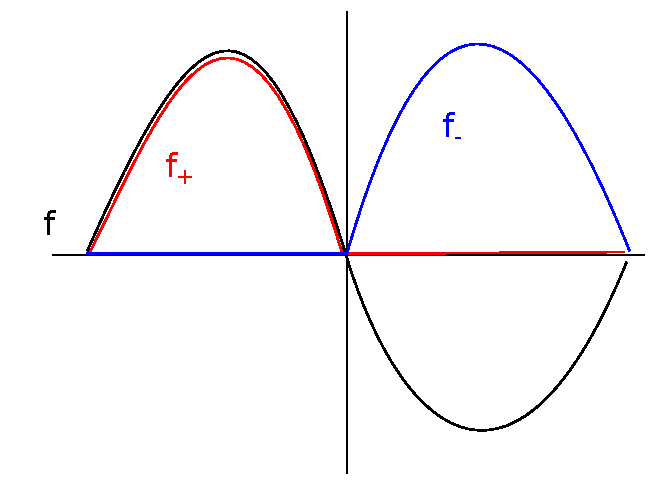
\includegraphics{img/14_fpm.pdf}
	  \caption{$f$, $f_-$ and $f_+$}
	\end{center}
\end{figure}

\begin{lemma}
  We have $f = f_+ - f_{-}$ and $\card{f} = f_{+} + f_{-}$.
  $f$ is measurable $\iff$ $f_-$ and $f_+$ are measurable.
\end{lemma}
\begin{definition}
  A function $S: X \to (-\infty, \infty) = \mathbb R$ is called a simple function iff
  $s(x) = \set{\alpha_1, \alpha_2, \ldots, \alpha_N}$ is a finite set.
  We set $\mathcal S = \setdef{s}{s \text{ is simple and measurable on } X}$.
  \[ \mathcal S_+ = \setdef{s: X \to [0, \infty)}{s \text{ is simple and measurable}} \]
  For $A \subseteq X$, we set $\chi_A(x) = \begin{cases} 1 & x \in A \\ 0 & x \in A^C \end{cases}$.
  We call $\chi_A$ the characteristic function of $A$.
\end{definition}

\begin{remark}
  Let $S: X \to \mathbb R$ be simple with $S(x) = \set{\alpha_1, \alpha_2, \ldots, \alpha_N}$ where $\alpha_j \neq \alpha_{j'}$ assuming $j \neq j'$.
  We define $A_j = s^{-1}(\set{\alpha_j})$. Then $s$ is measurable if and only if $A_j \in \mathcal A$ for $j=1,\ldots,N$ where $s$ is measurable
  $\implies s^{-1}(\underbrace{\set{\alpha_j}}_{\text{closed}}) \in \mathcal A$ if $A_j$ is measurable $s^{-1}([-\infty, t)) = \bigcup_{\alpha_j \in [-\infty, t)} s^{-1}(\set{\alpha_j}) \in \mathcal A$.
  $s = \sum_{j=1}^N \alpha_j \chi_{A_j}$ because $A_j \cap A_{j'} = \emptyset$ if $j \neq j'$ and
  $\bigcup_{j=1}^N A_j = X$ for $x \in A_{j'} \implies s(x) = \alpha_{j'}$ and $\sum_{j=1}^N \alpha_j \underbrace{\chi_{A_j}(x)}_{\delta_{j,j'}} = \alpha_{j'}$.
  $S$ is a linear combination of characteristic functions.
  \[ s = \sum_{j=1}]^N \alpha_j \chi_{A_j} \]
  Define $s' = \sum_{l=1}^M \beta_l \chi_{x}$.
  TODO content missing
\end{remark}

Let $s = \sum_{j=1}^N \alpha_j \chi_{A_j}$ be simple $A_j \in \mathcal A$.
We call the linear combination a standard representation of $s$ if $A_j \cap A_{j'} = \emptyset$ for $j \neq j'$.
A standard representation does not need to be unique.

\begin{figure}[!h]
  \begin{center}
    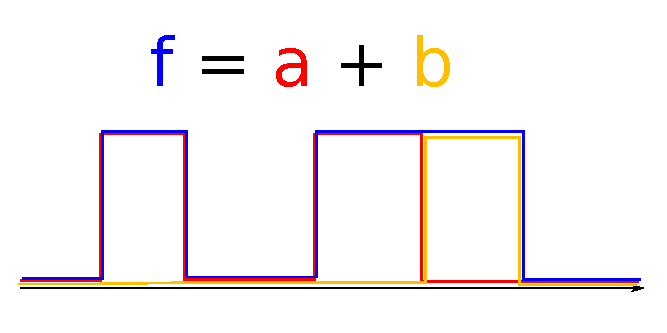
\includegraphics{img/15_sum_of_characteristic_functions.pdf}
    \caption{Sum of characteristic functions $a$ and $b$}
  \end{center}
\end{figure}

\begin{proposition}
  Let $f: X \to [0, \infty]$ be measurable. Then there exists a sequence $(S_n)_{n \in \mathbb N}$ of simple measurable functions
  $0 \leq s_1 \leq s_2 \leq \ldots \leq s_n \leq s_{n+1}$ such that $f(x) = \lim_{n\to\infty} s_n(x) \forall x \in X$.
  We say that $f$ is the pointwise limit of a monotone sequence of simple functions for $k = 0,1,\ldots, n2^n$ (with $n \geq 1$).
  We define $t_k^n = \frac{k}{2^n}$, $t_0^n = 0$ and $t_{n2^n}^n = \frac{n2^n}{2^n} = n$
\end{proposition}

\begin{figure}[!h]
  \begin{center}
    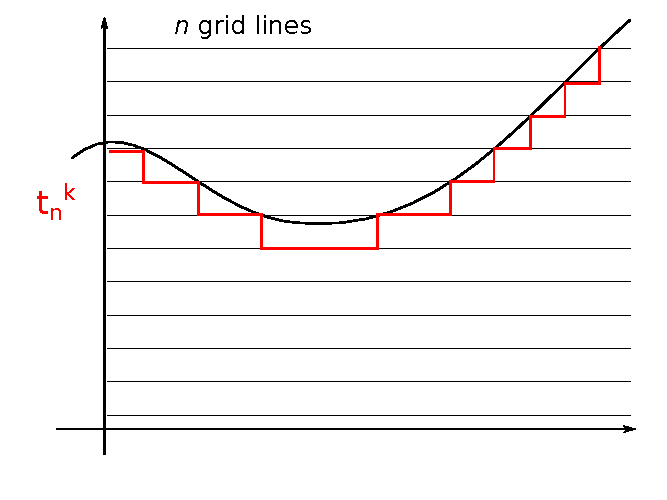
\includegraphics{img/16_construction_of_simple_functions.pdf}
    \caption{Construction of simple functions}
  \end{center}
\end{figure}

\begin{align*}
  t_k^n - t_{k-1}^n &= \frac{k}{2^n} - \frac{k-1}{2^n} = \frac{1}{2^n} = \triangle t^n \\
  t_k^n &= \frac{k}{2^n} - \frac{2k}{2^{n+1}} = t_{2k}^{n+1} < t_{2k+1}^{n+1} < t_{2k+2}^{n+1} = t_{k+1}^n \\
  M_k^n &= f^{-1}([t_{k-1}^n, t_k^n)) \text{ for } k = 1, \ldots, n2^n  \qquad M_k^n \in \mathcal A, M_\infty^n \in \mathcal A \\
  M_\infty^n &= f^{-1}([t_{n2^n}^n, \infty]) = f^{-1}([n,\infty])
\intertext{ because $f$ is measurable, because $\bigcup_{k=1}^{n2^n} [t_{k-1}^n, t_k^n) \cup [n,\infty] = [0, \infty] $}
  \bigcup_{k=1}^{n2^n} M_k^n \cup M_\infty^n &= X \text{ and } M_k^n \text{ are disjoint}
\end{align*}
We define $f_n(x) = \begin{cases} t_{k-1}^n & x \in M_{k}^n \text{ for } k = 1, \ldots, n2^n \\ n & x \in M_{\infty}^n \end{cases}$
which is simple and measurable because $M_k^n \in \mathcal A, M_{\infty}^n \in \mathcal A$.

\begin{description}
  \item[First case]
    \[ f(x) = \infty \implies x \in M_{\infty}^n \forall n \in \mathbb N \]
    \[ f_n(x) = n \to +\infty \text{ monotone} \]
  \item[Second case]
    \[ f(x) = t < \infty \text{ and we choose } n > t \]
    \[ \implies t \in [t_{k-1}^n, t_k^n) \text{ for exactly one } k \text{ and } f(x) = t, f_n(x) = t_{k-1}^n \implies x \in M_k^n \]
    \[ \card{f(x) - f_n(x)} = t - t_{k-1}^n < t_k^n - t_{k-1}^n = \frac{1}{2^n} \]
    So $f_n(x) \to f(x)$ as $n \to \infty$, $f_n \leq f_{n+1}$.
    \[ [t_{k-1}^n, t_k^n) = [t_{2k-2}^{n+1}, t_{2k-1}^{n+1}) \cup [t_{2k-1}^{n+1}, t_{2k}^{n+1}) \]
    \[ M_k^n = M_{2k-1}^{n+1} \cup M_{2k}^{n+1} \]
    if $x \in M_{k}^n$, $x \in M_{2k-1}^{n+1} \implies f_n(x) = t_{k-1}^n$ equivalent with $f_{n+1}(x) = t_{2k-2}^{n+1}$.
\end{description}

\dateref{2017/11/17}

\[ M_X^k = f^{-1}([t_{k-1}^n, t_k^n)) \qquad t_k^n = \frac{k}{2^n} \qquad \text{ where } k\in\set{0,\ldots,n2^n}, t_0^n = 0, t_{n2^n}^n = n \]
\[ f_1(x) = t_{k-1}^n \text{ if } x \in M_k^n, M_\infty^n = f^{-1}([n,\infty]) \]
\[ f_n(x) = n \text{ if } x \in M_X^n \]
\[ f_n(x) \leq f_{n+1}(x) \quad \forall n \in \mathbb N \text{ and } x \in X, f(x) = \infty \checkmark \]
\[ f(x) = t < \infty \]

a)
\begin{align*}
  t < n < n + 1 &\text{then } \exists k \in \set{0,\ldots,n2^n}: t_{k-1}^n \leq t < t_k^n \\
  \implies & x \in M_k^1 \text{ and } f_n(x) = t_{k-1}^n, \quad t_{k-1}^n = t_{2k-2}^{n+1} < t_{2k-1}^{n+1} < t_{2k}^{n+1} = t_k^n \\
  \implies & M_k^n = M_{2k-1}^{n+1} \cup M_{2k}^{n+1}
\end{align*}
\[
  f_{n+1}(x) = \begin{cases}
    t_{2k-2}^{n+1} = t_{n-1}^n & x \in M_{2k-1}^n \implies f_{n+1}(x) = f_n(x) \\
    t_{2k-1}^{n+1} & x \in M_{2k}^n \implies f_{n+1}(x) > f_n(x)
  \end{cases}
\]

b)
\[ n \leq t < n+1 \]
\[ x \in M_{\infty}^n, f_n(x) = n \]
\[ f_{n+1}(x) = t_{k}^{n+1} \text{ with } k \geq n2^{n+1} \implies f_{n+1}(x) = k \frac{1}{2^{n+1}} \geq n \frac{2^{n+1}}{2^{n+1}} = n = f_n(x) \]

c)
\[ t \geq n + 1 \]
\[ x \in M_{\infty}^{n+1} \text{ and } x \in M_{\infty}^n \]
\[ f_n(x) = n, f_{n+1}(x) = n+1 \]
\[ f_n(x) \leq f_{n+1}(x) \checkmark \]

\[ \mathcal M = \setdef{f: X \to [-\infty, \infty]}{f \text{ is measurable with respect to } \mathcal A} \]
\[ \mathcal M_{+} = \setdef{f \in \mathcal M}{f(x) \geq 0 \forall x \in X}, \xi, \xi_+ \checkmark \]
for $s \in \xi$ we know $s = \sum_{j=1}^{N} \alpha_j \chi_{A_j}$ with $A_j \cap A_{j'} = \emptyset$ for $j \neq j'$
sometimes we assume that $\bigcup_{j=1}^{N} A_j = X$ (set $A_0 = X \setminus (\bigcup_{j=1}^N A_j)$ and $\alpha_0 = 0$).
Sometimes we assume $\alpha_j \neq 0$ because we can omit a term $0$. $\chi_{A_j}$)

\begin{definition}[integration]
  Let $s \in \xi_+$, $s = \sum_{j=1}^N \alpha_j \xi_{A_j}$ ($A_j \in \mathcal A$ with $A_j \cap A_{j'} = \emptyset$ for $j \neq j'$).
  We define
  \[ \int_X s \, d\mu = \sum_{j=1}^N \alpha_j \mu(A_j) = \int s \, d\mu \] % IMPORTANT FORMULA!
\end{definition}

\begin{remark}
  The integral $\int_X s\, d\mu$ is independent of the chosen standard representation of $s$.
  Let \[ s = \sum_{j=1}^{N} \alpha_j \chi_{A_j} = \sum_{l=1}^{M} \beta_l \chi_{B_i} \]
  \[ X = \bigcup_{j=1}^N A_j = \bigcup_{l=1}^N B_l \implies A = \bigcup_{l=1}^M (A_j \cap B_l) \text{ disjoint}, B_l = \bigcup-{j=1}^N (B_l \cap A_j) \text{ disjoint} \]
  \[ \sum_{j=1}^N \alpha_j \mu(A_j) = \sum_{j=1}^N \alpha_j \mu\left(\bigcup_{l=1}^M (A_j \cap B_l)\right) = \sum_{j=1}^N \alpha_j \sum_{l=1}^M \underbrace{\mu(A_j \cap B_l)}_{\substack{= 0 \text{ iff } A_j \cap B_l = \emptyset \\ \text{ else } x \in A_j \cap B_l \implies a_j = s(x) = \beta_l}} \]
  \[ = \sum_{l=1}^{M} \beta_l \sum_{j=1}^{N} \mu (A_j \cap B_l) = \sum_{l=1}^M \beta_l \mu(\bigcup_{j=1}^N (A_j \cap B_l)) = \sum_{l=1}^M \beta_l \mu(B_l) \]
\end{remark}

\begin{proposition}[Proposition 5]
  Let $(X, \mathcal A, \mu)$ be a measure space.
  $f,g \in \xi_+$. Then
  \begin{enumerate}
    \item $\forall a \in \mathbb R^+: \int_X a f \, d\mu = a \int_X f \, d\mu$
    \item $\int_X (f + g) \, d\mu = \int_X f \, d\mu + \int_X g \, d\mu$
    \item $f(x) \leq g(x) \forall x \in X: (f \leq g) \text{ then } \int_X f \, d\mu \leq \int_X g \, d\mu$
  \end{enumerate}
\end{proposition}
\begin{proof}
  \begin{enumerate}
    \item \[ f = \sum_{j=1}^N \alpha_j \chi_{A_j} \qquad g = \sum_{l=1}^M \beta_l \chi_{B_l} \qquad \alpha_j, \beta_l \geq 0 \]
    \[ \int_X af \,d\mu = \sum_{j=1}^M a \alpha_j \mu(A_j) = a \sum_{j=1}^N \alpha_j \mu(A_j) = a \int_X fd\mu \]
    $f + g \in \xi_+$, $f + g \geq 0$, $f + g \in \mathcal M_+$.
    $f + g$ attains only finitely many function values $(f+g)(X) \subseteq \set{\alpha_0 + \beta_l, j \in \set{1,\ldots,N}, l\in\set{1,\ldots,M}}$.

    \[ = \sum_{l=1}^M \beta_l \mu(\bigcup_{j=1}^N (A_j \cap B_j)) = \sum_{l=1}^M \beta_l \mu(B_l) \checkmark \]
    \[ A_j = \bigcup_{l=1}^M (A_j \cap B_l) \qquad B_l = \bigcup_{j=1}^N (B_l \cap A_j) \]
    \begin{align*}
      (f+g)
        &= \sum_{j=1}^N \alpha_j \chi_{A_j} + \sum_{l=1}^M \beta_l \chi_{B_l} \\
        &= \sum_{j=1}^N \alpha_j \sum_{l=1}^M \chi_{A_j \cap B_l} + \sum_{l=1}^M \beta_l \sum_{j=1}^M \chi_{B_l \cap A_j} \\
        &= \sum_{j=1}^N \sum_{l=1}^M (\alpha_j + \beta_l) \chi_{\underbrace{A_j \cap B_l}_{\text{disjoint}}}
    \end{align*}
    \[
      (j,l) = (j', l') \implies (A_j \cap B_l) \cap (A_{j'} \cap B_{l'}) = \emptyset
    \]
    \begin{align*}
      \int_X (f+g) \, d\mu
        &= \sum_{j=1}^N \sum_{l=1}^M (\alpha_j + \beta_l) \mu(A_j \cap B_l) \\
        &= \sum_{j=1}^N \alpha_j \underbrace{\sum_{l=1}^M \mu(A_j \cap B_l)}_{\mu(A_j)} + \sum_{l=1}^M \beta_l \underbrace{\sum_{j=1}^N \mu(B_l \cap A_j)}_{\mu(B_l)} \\
        &= \int_X f \, d\mu + \int_X g \, d\mu
    \end{align*}
    \item[3.] \[
      f \leq g \implies g-f \in \xi_+ \implies \int_X (g-f) \, d\mu \geq 0
    \] \[
      \int_X g \, d\mu = \int_X (f + (g - f)) \, d\mu \stackrel{\text{by 2.}}{=} \int_X f \, d\mu + \underbrace{\int_X (g - f) \, d\mu}_{\geq 0} \geq \int_X f \, d\mu
    \]
  \end{enumerate}
\end{proof}

\dateref{2017/11/22}

Let $s \in \xi_+$.
\[ \int_X s \, d\mu = \sum_{i=1}^N \alpha_1 \mu(A_1) \text{ where } s = \sum_{i=1}^N \alpha_i \chi_{A_i} \]
$s = \xi_A$ and $A \in \mathcal A$.
\[ \int_X \chi_A \, d\mu = 1 \cdot \mu(A) = \mu(A) \]

\begin{proposition} % Proposition 6
  Let $s_n \in \xi_+$, $S \in \xi_+$ and $\forall x \in X: s_n(x) \leq s_{n+1}(x) \leq s(x)$
  and $s(x) = \lim_{n\to\infty} s_n(x)$. Then $\int_X s \, d\mu = \lim_{n\to\infty} \int_X s_n \, d\mu$
  where $\int_X s \, d\mu = \int_X \lim_{n\to\infty} s_n \, d\mu$.
\end{proposition}

\begin{proof}
  By monotonicity, it follows that
  \[ \int_X s_n \, d\mu \leq \int_X s_{n+1} \, d\mu \leq \int_X s \, d\mu \]
  \[ \implies \underbrace{\lim_{n\to\infty} \int_X s_n \, d\mu}_{\exists \in [0,\infty]} \leq \int_X s \, d\mu \]
  For the reverse inequality, we are going to show that $\forall \varepsilon > 0: \lim_{n\to\infty} \int_X s_n \, d\mu \geq (1 - \varepsilon) \int_X s \, d\mu$.
  Construct $g_n^{\varepsilon} \in \xi_+$ such that $g_n^\varepsilon \leq s_n$ and $\int_X g_n^{\varepsilon} \, d\mu \geq (1 - \varepsilon) \int_X s \, d\mu$

  Let $s = \sum_{j=1}^N \alpha_j \chi_{A_j} \geq 0$. Assume $\alpha_j > 0$ and $A_j \cap A_{j'} = \emptyset$ for $j \neq j'$.
  \[ A^\varepsilon(n,j) = \setdef{x \in A_j}{s_n(x) \geq (1 - \varepsilon) \alpha_j} \]
  because for $x \in A_j$ we have $s_n(x) \to s(x) = \alpha_j \implies \exists n \in \mathbb N: x \in A^\varepsilon(n,j)$.
  \[ A_j = \bigcup_{n=1}^\infty A^\varepsilon(n,j) \]
  because $s_{n+1} \geq s_n$ we have $x \in A^\varepsilon(n,j) \implies x \in A^\varepsilon(n+1,j)$.
  \[ A^\varepsilon(n,j) \subseteq A^\varepsilon(n+1,j) \]
  By a previous lemma, we get $\mu(A_j) = \lim_{n\to\infty} \mu(A^\varepsilon(n,j))$.
  We set $g_n = \sum_{j=1}^N (1 - \varepsilon) \alpha_j \chi_{A^\varepsilon}(n,j) \in \xi_X$.
  Then $\int_X g_n \, d\mu = (1 - \varepsilon) \sum_{j=1}^N \alpha_j \mu(A^\varepsilon(n,j))$.
  \[ \to_{n\to\infty} (1 - \varepsilon) \sum_{j=1}^N \alpha_j \mu(A_j) = (1 - \varepsilon) \int_X s \, d\mu \]
  \[ \lim_{n\to\infty} \int_X g_n \, d\mu = (1 - \varepsilon) \int_X s \, d\mu \]
  Show that $g_n(x) \leq s_n(x)$ holds.
  Suppose $x \not\in \bigcup_{j=1}^N A_j$ then $s(x) = 0$ and also $0 \leq s_n(x) \leq s(x) = 0 \implies s_n(x) = 0$.
  $x \not\in \bigcup_{j=1}^N A^\varepsilon(n,j) \implies g_n(x) = 0$.
  In this case $g_n(x) = s_n(x) = 0$ so $g_n(x) \leq s_n(x)$ holds.
  Let $x \in A_j$. Then $s_n(x)$,
  \begin{itemize}
  	\item if $x \in A^\varepsilon(n,j) \implies s_n(x) \geq (1 - \varepsilon) \alpha_j = g_n(x)$. QED.
  	\item if $x \in A_j \setminus A^\varepsilon(n,j)$. Then $g_n(x) = 0 \leq s_n(x)$.
  	  \[ \lim_{n\to\infty} \int_X g_n \, d\mu \leq \int_X s_n \, d\mu \]
  	  where $\lim_{n\to\infty} \int_X g_n \, d\mu = (1 - \varepsilon) \int_X s \, d\mu \forall \varepsilon > 0$.
  \end{itemize}
\end{proof}

\begin{definition}
  Let ($X, \mathcal A, \mu)$ be a measure space.
  \[ f: X \to [0, \infty] \text{ measurable} \]
  \[ \int_X f \, d\mu = \sup\setdef{\underbrace{\int_X s \, d\mu}_{\geq 0}}{s \in \xi_+ \text{ and } s \leq f}  \in [0,\infty] \]
\end{definition}

\begin{proposition}  % Proposition 7
  Let $f: X \to [0,\infty]$ be measurable. Let $s_n \in \xi_+$ with
  \[ s_(x) \leq s_{n+1}(x) \leq f(x) \text{ and } \lim_{n\to\infty} s_n(x) = f(x) \forall x \in X \]
  Then
  \[ \lim_{n\to\infty} \int_X s_n d\mu = \int_X f \, d\mu \]
\end{proposition}
\begin{proof}
  As before,
  \[ \int_X s_n \, d\mu \leq \int_X s_{n+1} \, d\mu \leq \lim_{n\to\infty} s_n \, d\mu \underbrace{\leq}_{\text{by def of $\int_X f \, d\mu$}} \int_X f \, d\mu \]
  It suffices to show that, $\lim_{n\to\infty} \int_X s_n \, d\mu \geq \int_X g \, d\mu \forall g \in \xi_+$ with $g \leq f$.
  We set $h_n = \min(g, s_n) \in \xi_+$. Obviously, $h_n \leq s_n \forall n \in \mathbb N$ because $s_n \leq s_{n+1}$.
  Hence, $h_n \leq h_{n+1}$. Moreover, $\lim_{n \to \infty} h_n(x) = \lim_{n\to\infty} \min\left(\underbrace{g(x)}_{\in \mathbb R}, h_n(x)\right) = \lim_{n\to\infty} \min(y, \psi_n)$ where $\psi_n = h_n(x)$ and $y = g(x)$.
  \begin{figure}[!ht]
    \begin{center}
      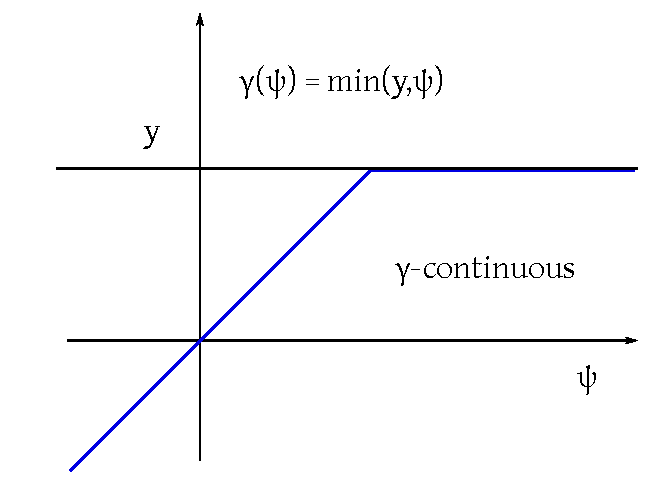
\includegraphics{img/17_psi.pdf}
      \caption{$\psi$ in the proof of Proposition 7}
    \end{center}
  \end{figure}
  \begin{align*}
    \lim_{n\to\infty} \min(y, \psi_n)
      &= \min(g(x), \lim_{n\to\infty} s_n(x)) \\
      &= \min(g(x), f(x)) = g(x) \\
  \end{align*}
  \[ h_n(x) \to g(x) \forall x \in X \]
  by proposition 6:
  \[ \implies \lim_{n\to\infty} \int_X h_n \, d\mu = \int_X f \, d\mu \]
  Because $h_n \leq s_n \implies \lim_{n\to\infty} \int_X s_n \, d\mu \geq \int_X g \, d\mu$.
  \[ \implies \lim_{n\to\infty} \int_X \, d\mu \geq \int_X f \, d\mu \]
\end{proof}

\begin{proposition} % 8
  Let $(X, \mathcal A, \mu)$ be a measure space, $f, g: X \to [0,\infty]$ be measurable and let $\alpha \geq 0$. Then
  \begin{enumerate}
  	\item $\int_X \alpha f \, d\mu = \alpha \int_X f \, d\mu$
  	\item $\int_X(f+g) \, d\mu = \int_X f \, d\mu + \int_X g \, d\mu$
  	\item If $f(x) \leq g(x) \forall x \in X$ then $\int_X f \, d\mu \leq \int_X g \, d\mu$.
  \end{enumerate}
\end{proposition}

\begin{proof}
   Let $(s_n)_{n \in \mathbb N}$, $(\sigma_n)_{n\in\mathbb N}$ be monotone sequences of simple functions with $\lim_{n\to\infty} s_n(x) = f(x)$ and $\lim_{n\to\infty} \sigma_n(x) = g(x)$ (Proposition~4). The last proposition~7: $\lim_{n\to\infty} s_n \, d\mu = \int_X f \, d\mu$ and $\lim_{n\to\infty} \int_X \sigma_n \, d\mu = \int_X g \, d\mu$.
   \[ \int_X \alpha f \, d\mu \underbrace{=}_{\text{by Prop.~7}} \lim_{n\to\infty} \int_X \alpha S_n \, d\mu = \lim_{n\to\infty} \alpha \int_X s_n \, d\mu = \alpha \int_X f \, d\mu \]
   \[ \int_X (f+g) \, d\mu = \lim_{n\to\infty} \int_X \underbrace{(S_n + \sigma_n)}_{\in \xi_+} \, d\mu \]
   \[ \lim_{n\to\infty} f \, d\mu = \sup\underbrace{\setdef{\int_X s \, \mu}{s \in \xi_+, s \leq f}}_{\subseteq \setdef{\int_X s \, d\mu}{s \in \xi_+, s \leq g}} \]
   \[ \sup\setdef{\int_X s \, d\mu}{s \in \xi_+, s \leq g} = \int_X g \, d\mu \]
\end{proof}

\index{Integrable function on $X$}
\begin{definition}
  Let $f \in \mathcal M$, $f_+ = \max(f, 0) \in \mathcal M_+$ and $f_- = -\min(f, 0) \in \mathcal M_+ \forall x \in X$.
  Either $f_+(x) = 0$ or $f_-(x) = 0$ holds.
  \[ f = f_+ - f_- \text{ and } \card{f} = f_+ + f_- \]
  \[ f(x) = f_+(x) - f_-(x) \text{ always makes sense} \]
  Assume that $\int_X f_+ \, d\mu < \infty$ and $\int_X f_- \, d\mu < \infty$.
  Then we set $\int_X f \, d\mu = \int_X f_+ \, d\mu - \int_X f_- \, d\mu$.
  A measurable function satisfying the previous assumption (integral $f_+$ and $f_-$ are finite)
  is called \emph{integrable on $X$}.
\end{definition}

\begin{remark}
  If $\int_X f_+ \, d\mu < \infty$ and $\int_X f_- \, d\mu < \infty$, then
  \[ \int_X \underbrace{\card{f}}_{\geq 0} \, d\mu = \int_X (f_+ + f_-) \, d\mu = \int_X f_+ \, d\mu + \int_X f_- \, d\mu \]
  On the other hand, if $\int_X \card{f} \, d\mu < \infty$. Then $\int_X f_+ \, d\mu$ % TODO
\end{remark}

$f \in \mathcal M$ is integrable iff $\int_X \card{f} \, d\mu < \infty$.
\begin{itemize}
  \item We could define $\int_X f \, d\mu$ if only one condition $\int_X f_+ \, d\mu < \infty$ or $\int_+ f_- \, d\mu < \infty$ holds.
  \item
    Let $A \subseteq X$, $A \in \mathcal A$. We set for $f \in \mathcal M$, $\int_A f\, d\mu = \int_X \underbrace{\chi_A f}_{\in \mathcal M} \, d\mu$
    if $\chi_A f$ is integrable. We get the same integral, if we consider the measure space ($A, \mathcal A_A, \mu_A$) where
    $\mathcal A_A = \setdef{B \cap A}{B \in \mathcal A}$ is a $\sigma$-algebra and
    $\int_A f_A \, d\mu_A = \int_X \chi_A f \, d\mu$.
    For $A' \subseteq A, A' \in \mathcal A_A$ we set $\mu_A(A') = \mu(A')$,
    $f: X \to [-\infty, \infty]$ can be restricted to $A$, i.e. $f_A = \left.f\right|_A$.
    $f_A: A \to [-\infty, \infty]$ is measurable with respect to $\mu_A$.
  \item % TODO: board says "definition continued", what? which one?
    We set $\mathcal L^1(X, \mathcal A, \mu) = \mathcal L^1(X) = \setdef{f \in \mathcal M}{f \text{ is integrable on $X$, i.e., } \int_X \card{f} \, d\mu < \infty}$
\end{itemize}

\index{Almost everywhere on a measure}
\index{Holds almost everywhere on a measure}
\index{Holds for almost all elements of a measure}
\begin{definition}
  Let ($X, \mathcal A, \mu$) be a measure space and $x \in X$.
  We consider $P(x)$ a statement which can be true or false.
  We say that $P(x)$ \emph{holds almost everywhere on $X$} or \emph{holds for almost all $x \in X$} if
  \[ \mu(\setdef{x \in X}{\neq P(x)}) = 0 \]
  Almost everywhere iff everywhere expect on a set of measure 0.

  $f: X \to [0, \infty]$.
  \[ \int f\, d\mu = 0 \iff f(x) = 0 \text{ a. e. } on X \]
  where a.e. stands for \emph{almost everywhere}.
\end{definition}

\dateref{2017/11/24}

\begin{lemma} % Lemma 5
  Let $f \in \mathcal M_+$, $f: X \to [0,\infty]$.
  \[ \implies \int_X f \, d\mu = 0 \iff \mu(\underbrace{\setdef{x \in X}{f(x) > 0}}_{P}) = 0 \]
\end{lemma}
\begin{proof}
  % NOTE: \xi_+ is a non-negative simple function
  Suppose $P = \setdef{x \in X}{f(x) > 0}$ and $\mu(P) = 0$.
  Let $s \in \xi_+$ with $0 \leq s \leq f$. Then for all $x \in X \setminus P$,
  we have $0 \leq s(x) \leq f(x)$. Because $x \in X \setminus P$, $f(x) = 0$ holds.
  Hence $s(x) = 0$.
  \[ s = \sum_{i=1}^N \alpha_i \chi_{A_i} \text{ with } \alpha_i > 0 \text{ and } A_i \cap A_j = \emptyset \text{ if } i = i' \]
  \[ A_i \in \mathcal A \]
  Then $s(x) > 0$ if $x \in A_i$ for one $i \in \set{1, \ldots, N}$.
  $x \in A_i \implies s(x) > 0 \implies f(x) > 0 \implies x \in P$.
  So $A_i \subseteq P$. Therefore $\mu(A) \leq \mu(P) = 0$, so $\mu(A_i) = 0$.
  \[ \int_X s \, d\mu = \sum_{i=1}^N \alpha_i \underbrace{\mu(A_i)}_{=0} = 0 \]
  \[ \implies \int_X f \, d\mu = \sup\setdef{\int_X s \, d\mu}{s \in \xi_+, 0 \leq s \leq f} = 0 \]

  We also need to prove the other direction:
  Suppose $\int_X f \, d\mu = 0$ and let $P = \setdef{x \in X}{f(x) > 0}$.
  \[ P_n = \setdef{x \in X}{f(x) \geq \frac1n} \in \mathcal A \]
  \[ x \in P \iff \exists n \in \mathbb N: x \in P_n \implies P = \bigcup_{n=1}^\infty P_n \]
  $P_n \subset P_{n+1}$. Consequently $\mu(P) = \lim_{n\to\infty} \mu(P_n)$.
  Assume $\mu(P) > 0$. Then $\exists n \in \mathbb N$. $\mu(P_n) > 0$.
  Let $s = \frac1n \cdot \chi_{P_n} \in \xi_+$.
  $x \in P_n: \frac1n = s(x) \leq f(x), x \not\in P_n: s(x) = 0 \leq f(x)$.
  So $s \leq f$ on $X$ and
  \[ \int_X s \, d\mu = \frac1n \underbrace{\mu(P_n)}_{>0} > 0 \implies \int_x f \, d\mu > 0 \]
  This is a contradiction and our proof is complete.
\end{proof}

\begin{remark}
  Let $f: X \to [0,\infty]$ and $\int_X f \, d\mu < \infty$.
  Then for $S = \setdef{x \in X}{f(x) = \infty}$ (where $S$ stands for \emph{singularity})
  it holds that $\mu(S) = 0$
\end{remark}
\begin{proof}
  because otherwise $n \chi_S$ is a simple function below $f$ and
  \[
  	\int_X f \, d\mu \geq \int_X n \lambda_S \, d\mu = \underbrace{n \cdot \mu(\chi_S)}_{\to +\infty \text{ as } n\to\infty}
    \implies \int_X f \, d\mu = +\infty
  \]
  leading to a contradiction.
\end{proof}
\begin{remark}
  We frequently use the following argument:
  Let $f \in \mathcal M_+$ and $E \in \mathcal A$ with $\mu(E) = 0$.
  Let
  \[
  	\tilde f(x) \coloneqq \begin{cases}
  	  f(x) & x \not\in E \\
  	  0 & x \in E
  	\end{cases}
  \]
  The equivalent definition is given by $\tilde f \coloneqq f \cdot \chi_{X \setminus E} \in \mathcal M^+$.
  Then $\int_X f \, d\mu = \int_X \tilde f \, d\mu$.
\end{remark}
\begin{proof}
  We can prove this using $g \coloneqq f - \tilde f$.
  \[
  	g(x) = \begin{cases}
  	  0   & x \not\in E \\
  	  f(x) \geq 0   & x \in E
  	\end{cases}
  \]
  $g \in \mathcal M_+$ and $g(x) > 0 \implies x \in E$
  \[ \mu(\setdef{x \in X}{g(x) > 0}) = 0 \]
  Then by Lemma~5,
  \[ \int_X g \, d\mu = 0 \implies \text{ with } f = g + \tilde f \text{ and } \int_X f \, d\mu = \underbrace{\int_X g \, d\mu}_{=0} + \int_X \tilde f \, d\mu \]
  \[ \implies \int_X f \, d\mu = \int_X \tilde f \, d\mu \]
\end{proof}
\begin{lemma} % Lemma 6
  Let $f, g \in \mathcal M_+$ and $f = g$ almost everywhere on $X$.
  Then $\int_X f \, d\mu = \int_X g \, d\mu$.
\end{lemma}
\begin{proof}
  \[ E = \setdef{x \in X}{f(x) \neq g(x)} \]
  $\mu(E) = 0$. We set $\tilde f = f \cdot \chi_{X \setminus E}$.
  $\tilde g = g \cdot \chi_{X \setminus E}$.
  \[ \implies \tilde f = \tilde g \implies \int_X \tilde f \, d\mu = \int_X \tilde g \, d\mu \]
  By the previous remark, it holds that
  \[ \int_X f \, d\mu = \int_X \tilde f \, d\mu = \int_X \tilde g \, d\mu = \int_X g \, d\mu \]
\end{proof}

Let $f,g \in \mathcal L^1(X)$, i.e. $\int_X \card{f} \, d\mu < \infty$ and $\int_X \card{g} \, d\mu < \infty$.
We define an equivalence relation on $\mathcal L(X)$.
\[ f \sim g \iff \int_X \card{f - g} \, d\mu = 0 \iff \card{f - g} = 0 \text{ a.e. on } X \iff f = g \text{ a.e. on } X \]
It is trivial to show that $\sim$ is an equivalence relation (only transitivity is a tiny challenge).
We let
\[ L^1(x) \coloneqq \setdef{\overline{f}}{f \in \mathcal L^1(x), \overline{f} \text{ is the equivalence class of $f$ with respect to $\sim$}} \]

We will see: $L^1(x)$ is a vector space.
$\norm{\overline{f}}_{L^1} = \int_X \card{f} \, d\mu$ for some $f \in \overline{f}$.
$\norm{\cdot}_{L^1}$ is a norm on $L^1(X)$.

We discuss this norm briefly:
\[ \norm{\overline{f}}_{L^1} = 0 \iff \int_X \card{f} \, d\mu = 0 \iff f = 0 \text{ a.e. on } X \iff \overline{f} = \overline{0} \]

Triangle inequality:
\[ \norm{\overline{f+g}}_{L^1} = \int_X \card{f+g} \, d\mu \leq \int_X (\card{f} + \card{g}) \, d\mu = \norm{\overline{f}}_{L^1} + \norm{\overline{g}}_{L^1}  \]
The relation $\leq$ holds because of monotonicity.

\dateref{2017/11/29}

\[ f: X \to [-\infty, \infty] \qquad f = f_+ - f_- \qquad \card{f} = f_+ + f_- \]
\[ \int_X \card{f} \, d\mu < \infty \iff \int_X f_+ \, d\mu < \infty \qquad \int_X f_- \, d\mu < \infty \iff f \text{ integrable} \]
\[ \int_X f \, d\mu = \int_X f_+ \, d\mu - \int_X f_- \, d\mu \]

\begin{lemma} % Lemma 7
  Let $(X, \mathcal A, \mu)$ be a measure space $f_1, f_2, g_1, g_2 \in \mathcal M_+$ and $f_1 - f_2 = g_1 - g_2$ on $X$
  and $f_1, f_2, g_1, g_2$ are supposed to be integrable. Then $\int_X f_1 \, d\mu - \int_X f_2 \, d\mu = \int_X g_1 \, d\mu - \int_X g_2 \, d\mu$.
\end{lemma}
\begin{proof}
  \begin{align*}
    f_1 - f_2 &= g_1 - g_2 \implies \underbrace{f_1 + g_2}_{\in \mathcal M_+} = \underbrace{g_1 + f_2}_{\in \mathcal M_+} \\
      &\implies \int_X (f_1 + g_2) \, d\mu = \int_X f_1 \, d\mu + \int_X g_2 \, d\mu \\
      &\implies \int_X (g_1 + f_2) \, d\mu = \int_X g_1 d\mu + \int_X f_2 \, d\mu \\
  \intertext{all integrals are finite}
      &\implies \int_X f_1 \, d\mu - \int_X f_2 \, d\mu = \int_X g_1 \, d\mu - \int_X g_2 \, d\mu
  \end{align*}
\end{proof}

\begin{proposition} % Proposition 9
  Let $f, g$ be integrable on $X$, $f: X \to [-\infty, \infty]$, $g: X \to [-\infty, \infty]$.
  Let $\alpha \in \mathbb R$. Then
  \begin{enumerate}
    \item $\alpha f$ and $f + g$ are integrable functions.
    \item $\int_X \alpha f \, d\mu = \alpha \int_X f \, d\mu$
    \item $\int_X (f + g) \, d\mu = \int_X f \, d\mu + \int_X g \, d\mu$
    \item $f \leq g$ on $X$ then $\int_X f \, d\mu \leq \int_X g \, d\mu$
    \item $\card{\int_X f \, d\mu} \leq \int_X \card{f} \, d\mu$
  \end{enumerate}
\end{proposition}
\begin{proof}
  \begin{enumerate}
    \item
      \begin{align*}
        \int_X \card{\alpha f} \, d\mu &= \int_X \underbrace{\card{\alpha} \card{f}}_{\in \mathcal M_+} \, d\mu \\
          &= \card{\alpha} \underbrace{\int_X \card{f} \, d\mu}_{< \infty} < \infty
      \end{align*}
      so $\alpha f$ is integrable.
      \[ \int_X \card{f+g} \, d\mu \leq \int_X\left(\card{f} + \card{g}\right) \, d\mu = \int_X \card{f} \, d\mu + \int_X \card{g} \, d\mu > \infty \]
      The inequality $\leq$ holds because of monotonicity for functions in $\mathcal M_+$.

    \item $\alpha = 0 \implies \alpha f = 0$.
      \[ \int_X \alpha f \, d\mu = 0 \qquad \alpha \int_X f \, d\mu = 0 \]
      
      Consider $\alpha > 0$.
      \[
        (\alpha f)_+ = \begin{cases}
          \alpha f(x) & \alpha f(x) \geq 0 \\
          0 & \alpha f(x) < 0
        \end{cases}
      \] \[
        = \alpha \begin{cases}
          f(x) & f(x) \geq 0 \\
          0 & f(x) < 0
        \end{cases} = \alpha f_+
      \]
      Analogously: $(\alpha f)_- = \alpha \cdot f_-$.
      \begin{align*}
        \int_X (\alpha f) \, d\mu &= \int_X (\alpha f)_+ \, d\mu - \int_X (\alpha f)_- \, d\mu \\
          &= \alpha \int_X f_+ \, d\mu - \alpha \int_X f_- \, d\mu \\
          &= \alpha \left(\int_X f \, d\mu - \int_X f_- \, d\mu\right) \\
          &= \alpha \int_X f \, d\mu
      \end{align*}

      Consider $\alpha < 0$.
      \[
        (\alpha f)_+(x) = \begin{cases}
          \alpha f(x) & \alpha f(x) \geq 0 \\
          0 & \text{else}
        \end{cases}
      \] \[
        \alpha \begin{cases}
          f(x) & f(x) \leq 0 \\
          0 & \text{ else}
        \end{cases}
        = \alpha (-f_-)
      \] \[
        (\alpha f)_-(x) = \begin{cases}
          -\alpha f(x) & \alpha f(x) \leq 0 \\
          0 & \text{ else}
        \end{cases}
      \] \[
        -\alpha \begin{cases}
          f(x) & f(x) \geq 0 \\
          0 & \text{ else}
        \end{cases} = (-\alpha) f_+
      \]
      \begin{align*}
        \int_X \alpha f \, d\mu &= \int_X (\alpha f)_+ \, d\mu - \int_X (\alpha f)_- \, d\mu \\
          &= \int_X \underbrace{(-\alpha) (-\alpha) f_-}_{\in \mathcal M_+} \, d\mu - \int_X \underbrace{(-\alpha) f_+}_{\in \mathcal M_+} \, d\mu \\
          &= -\alpha \int_X f_- \, d\mu + \alpha \int_X f_+ \, d\mu \\
          &= \alpha \int_X f \, d\mu
      \end{align*}

    \item
      \begin{align*}
        f+g &= (f+g)_+ - (f+g)_- \\
        f+g &= f_+ - f_- + g_+ - g_- = (f_+ + g_+) - (f_- + g_-)
      \end{align*}
      Now we apply Lemma~6:
      \begin{align*}
        \int_X (f+g)_+ \, d\mu - \int_X (f + g)_- \, d\mu
          &= \int_X (f_+ + g_+) \, d\mu - \int_X (f_- + g_-) \, d\mu \\
          &= \int_X f_+ \, d\mu + \int_X g_+ \, d\mu - \int_X f_- \, d\mu - \int_X g_- \, d\mu \\
          &= \left(\int_X f_+ \, d\mu - \int_X f_- \, d\mu\right) + \left(\int_X g_+ \, d\mu - \int_X g_- \, d\mu\right) \\
          &= \int_X f\, d\mu + \int_X g \, d\mu \checkmark
      \end{align*}

    \item
      \[ f \leq g \implies g-f \geq 0 \implies g-f = (g-f)_+ \land (g-f)_- = 0 \]
      \[ \int_x (g-f) \, d\mu = \int_X (g-f)_+ \, d\mu \geq 0 \]
      \[ \int_x (g-f) \, d\mu = \int_X (g + (-f)) \, d\mu = \int_X g \, d\mu + \int_X (-f)\, d\mu = \int_X g \, d\mu - \int_X f \, d\mu \checkmark \]

    \item
      \[ f \leq \card{f} \stackrel{(4)}{\implies} \int_X f \, d\mu \leq \int_X \card{f} \, d\mu \]
      \[ -f \leq \card{f} \stackrel{(4)}{\implies} \int_X (-f) \, d\mu = -\int_X f \, d\mu \leq \int_X \card{f} \, d\mu \]
      \[ \implies \card{\int_X f \, d\mu} \leq \int_X \card{f} \, d\mu \]
  \end{enumerate}
\end{proof}

\subsection{Convergence theorems}

\begin{theorem}[Monotone convergence theorem]  % important for exam! (like everything that has a name)
  By Beppo Levi (1875--1961)

  Let $f_n, f \in \mathcal M_+$ and $f_n(x) \leq f_{n+1}(x) \leq f(x)$ (monotonicity) for all $n \in \mathbb N$ and for almost every $x \in X$.
  Suppose $\lim_{n\to\infty} f_n(x) = f(x)$ almost everywhere on $X$.
  Then $\lim_{n\to\infty} f_n \, d\mu = \int_X f \, d\mu = \int_X \lim_{n\to\infty} f_n \, d\mu$.
\end{theorem}
\begin{proof}
  First, we replace almost everywhere by $\forall x \in X$.
  $\left(\int_X f_n \, d\mu\right)_{n\in\mathbb N}$ is a monotone sequence in $[0,\infty]$
  $\lim_{n\to\infty} \int_X f_n \, d\mu$ exists in $[0,\infty]$ and by monotonicity of the integral
  \[ f_n \leq f \implies \lim_{n\to\infty} \int_X f_n \, d\mu \leq \int_X f \, d\mu \]
  We know by Proposition~4: $\exists (g_n^k)_{k \in \mathbb N}$ for every $n \in \mathbb N$
  such that $g_n^k \in \xi_+$, $g_n^k \leq g_n^{k+1} \leq f_n$ and $f_n(x) = \lim_{k\to\infty} g_n^k(x) \forall x \in X$.
  \[ h_n \coloneqq \max\set{g_1^n, g_2^n, \ldots, g_n^n} \in \xi_+ \]
  \[ h_{n+1} \geq \underbrace{g_i^{n+1}}_{\text{for } i \in \set{1,\ldots,n+1}} \stackrel{\substack{\text{by monotonicity} \\ \text{of } (g_i^k)}}{\geq} g_i^n \qquad \text{ for } i = 1,\ldots,n \]
  So $h_{n+1} \geq \max\set{g_1^n, g_2^n, \ldots, g_n^n} = h_n$ where $(h_n)_{n \in \mathbb N}$ is a nondecreasing sequence of simple functions.
  \[ g_i^n \leq f_i \stackrel{\substack{\text{by monotonicity} \\ \text{of } (f_n)}}{\leq} f_n \leq f \text{ for } i = 1,\ldots,n \]
  \[ \stackrel{\max}{\implies} h_n \leq f_n \leq f \text{ on } X \]

  \begin{claim}$\lim_{n\to\infty} h_n(x) = f(x) \forall x \in X$.\end{claim}
  \begin{proof}
    Case 1 is assuming $f(x) < \infty$.

    Let $\varepsilon > 0$ be given. Choose $N_1 \in \mathbb N$ sufficiently large such that
    \[ \underbrace{\card{f_n(x) - f(x)} < \frac{\varepsilon}{2}}_{\text{pointwise convergence}} \text{ for all } n \geq N_1 \]
    Choose $N_2 \in \mathbb N$ such that $f_{N_1}(x) - g_{N_1}^{N_2}(x) < \frac{\varepsilon}{2}$.
    It is less than $\frac{\varepsilon}{2}$, because $g_{N_1}^k$ approximates $f_{N_1}$.
    Let $n \geq \max(N_1, N_2)$.
    \[ \underbrace{f(x) - h_n(x)}_{\geq 0} = \underbrace{f(x) - f_{N_1}(x)}_ {< \frac\varepsilon2} + f_{N_1}(x) - h_n(x) \leq \frac\varepsilon2 + f_{N_1}(x) - g^n_{N_1}(x) \]
    Then by monotonicity of $g_{N_1}^k$:
    \[ \leq \frac\varepsilon2 + f_{N_1}(x) - g_{N_1}^{N_2}(x) < \frac\varepsilon2 + \frac\varepsilon2 = \varepsilon \]
    So $f(x) = \lim_{n\to\infty} h_n(x)$

    Case 2 is assuming $f(x) = \infty$.

    Let $c > 0$ be given. $f_n(x) \to f(x)$. Choose $N_1 \in \mathbb N$ such that $n \geq N_1 \implies f_n(x) > 2c$. $g_{N_1}^k \to f_{N_1}$.
    Choose $N_2 \in \mathbb N$ such that $g_{N_1}^{N_2}(x) > c$ for $n \geq \max(N_1, N_2) \cdot h_n(x) \geq g_n^{N_2}(x) \geq g_{N_1}^{N_2}(x) > c$.
    \[ \lim_{n\to\infty} h_n(x) = \infty = f(x) \]
  \end{proof}

  Proposition 7 implies that $\int_X f \, d\mu = \lim_{n\to\infty} \int_X h_n \, d\mu$.
  \[ \int_X f \, d\mu = \lim_{n\to\infty} \int_X h_n \, d\mu \underbrace{\leq}_{h_n \leq f_n} \lim_{n\to\infty} \int_X f_n \in d\mu \leq \int_X f \, d\mu \checkmark \]
  Because LHS and RHS are the same, all inequalities must be equalities.

  Regarding the almost everywhere situation:
  Let $X' = \setdef{x \in X}{f_n(x) \leq f_{n+1}(x) \text{ and } f(x) = \lim_{n\to\infty} f_n(x)}$.
  \[ E = X \setminus X' \qquad \mu(E) = 0 \qquad \tilde f_n = f_n \cdot \chi_{X'} \qquad \tilde f = f \cdot \chi_{X'} \]
  Then $\int_X f_n \, d\mu = \int_X \tilde f_n \, d\mu$ because $\tilde f_n = f_n$ almost everywhere.
  \[ \int_X \tilde f \, d\mu = \int f \, d\mu \]
  $\tilde f_n$ and $\tilde f$ satisfy the condition of the theorem.
  \[ \forall x \in X \implies \int_X f \, d\mu = \int_X \tilde f \, d\mu = \lim_{n\to\infty} \int_X \tilde f_n \, d\mu = \lim_{n\to\infty} \int_X f_n \, d\mu \]
\end{proof}

\begin{corollary}[Beppo-Levi Theorem] % Corollary 2
  Let $f_n \in \mathcal M_+$ and consider $g = \sum_{n=1}^\infty f_n$. $\sigma_N = \sum_{n=1}^N f_n$, $g = \sup\setdef{\sigma_N}{N \in \mathbb N}$ so $g \in \mathcal M_+$.
  Then $\int_X g \, d\mu = \sum_{n=1}^\infty f_n \, d\mu = \sum_{n=1}^\infty \int_X f_n \, d\mu = \lim_{N\to\infty} \sum_{n=1}^N \int_X f_n \, d\mu$
\end{corollary}
\begin{proof}
  Apply monotone convergence theorem to sequence $\sigma_N$.
\end{proof}

An important conclusion:

Let $(X, \mathcal A, \mu)$ be a measure space, $f \in \mathbb M_+$.
We define $\nu: \mathcal A \to [0, \infty]$ as $\nu(A) = \int_A f \, d\mu = \int_X f \cdot \chi_A \, d\mu$.
Then $\nu$ is a measure on $\mathcal A$.

If $f$ is the constant function $1$, then we get $\nu = \mu$.

\[ \nu(\emptyset) = 0 \checkmark \]
We only need to prove $\sigma$-additivity of $\nu$:
Let $(A_n)_{n\in\mathbb N}$.
\[ A_n \in \mathcal A, A_n \cap A_m = \emptyset \text{ if } n \neq n' \text{ show that } \nu(A) = \sum_{n=1}^\infty \nu(A_n) \]
\[ \chi_A = \begin{cases} 1 & x \in A_n \text{ for exactly one } n \\ 0 & \text{ else} \end{cases} \]
\[ \sum_{n=1}^\infty \chi_{A_n} = \begin{cases} 1 & x \in A_n \text{ for one } n \in \mathbb N \\ 0 & x \not\in \bigcup_{n=1}^\infty A_n \end{cases} \]
So $\chi_A = \sum_{n=1}^\infty \chi_{A_n}$.
\[ \sum_{n=1}^\infty \nu(A_n) = \sum_{n=1}^\infty \int_X f \cdot \chi_{A_n} \, d\mu \stackrel{\text{Beppo Levi}}{=} \int_X f \sum_{n=1}^\infty \chi_{A_n} \, d\mu = \int_X f \chi_{A} \, d\mu = \nu(A) \checkmark \]

\dateref{2017/12/06}

TODO I was missing the first half an hour

\begin{theorem}[Fatou's Lemma]
  Pierre Fatou (1878-1929)

  Let $f_n \in \mathcal M_+$ and we set $f = \liminf_{n\to\infty} f_n \in \mathcal M_+$ (is known) ($\coloneqq \lim_{n\to\infty}(\inf\setdef{f_k}{k \geq n})$).
  \[ \implies \int_x f \, d\mu \leq \liminf_{n\to\infty} \int_X f_n \, d\mu \]
\end{theorem}
\begin{proof}
  \[ g_n = \inf\setdef{f_k}{k \geq n} \]
  $g_n$ is non-decreasing, measurable.
  Monotone convergence implies that $f = \lim_{n\to\infty} g_n$ limit is pointwise, monotone.
  \[ \int_X f \, d\mu = \lim_{n\to\infty} \int_X g_n \, d\mu = \liminf_{n\to\infty} \int_X g_n \, d\mu \underbrace{\leq}_{g_n \leq f_n} \liminf_{n\to\infty} \int_X f_n \, d\mu \]
\end{proof}

\begin{theorem}[Dominated convergence theorem, Lebesgue] % THeorem 3
  Let $f_n \in \mathcal M$ and $f \in \mathcal M$ with $f(x) = \lim_{n\to\infty} f_n(x)$ almost everywhere on $X$.
  Suppose that $\exists g \in \mathcal M_+$ with $0 \leq \int_x f \, d\mu < \infty$ ($g \in \mathcal L^1(x)$) and $\card{f_n(x)} \leq g(x)$ almost everywhere on $X$ $\forall n \in \mathbb N$.
  $g$ is the so-called \emph{integratable majorant}.

  Then $f_n \in \mathcal L^1(X) \forall n \in \mathbb X$ and $\lim_{n\to\infty} \int_X \card{f_n - f} \, d\mu = 0$. $f \in \mathcal L^1(X)$ and $\int_x f \, d\mu = \lim_{n\to\infty} \int_X f_n \, d\mu$.
\end{theorem}
\begin{proof}
  \[ \card{f_n} \leq g \qquad \card{f} = \lim_{n\to\infty} \card{f_n} \leq g \text{ almost everywhere on } X \]
  i.e. $\int_X \card{f_n} \, d\mu \leq \int_X g \, d\mu < \infty$ and $\int_x \card{f} \, d\mu \leq \int_X g \, d\mu < \infty$.
  \[ \card{f_n} \leq g \land \card{f} \leq g \implies \card{f_n - f} \leq \card{f_n} + \card{f} \leq 2g \]
  \begin{align*}
    \underbrace{2g - \card{f_n - f}}_{\in \mathcal M_+} \geq 0 \text{ Fatou }
    &\implies \int_X \liminf_{n\to\infty} (2g - \underbrace{\card{f_n - f}}_{\to 0}) \, d\mu \\
    &\leq \liminf_{n\to\infty} \int_X (2g - \card{f_n - f}) \, d\mu \\
    &= \liminf_{n\to\infty} (\int_X 2g \, d\mu - \underbrace{\int_X (f_n - f) \, d\mu}_{\geq 0}) \\
    &= \int_X 2g \, d\mu - \limsup_{n\to\infty} \int_X \card{f_n - f} \, d\mu \\
  0 &\leq -\limsup_{n\to\infty} \int_X \card{f_n - f} \, d\mu \iff \limsup_{n\to\infty} \int_X \card{f_n - f} \, d\mu \leq 0 \\
    &\leq \liminf_{n\to\infty} \underbrace{\int_X \card{f_n - f} \, d\mu}_{\geq 0} \leq \limsup_{n\to\infty} \int_X \card{f_n - f} \, d\mu \leq  0 \\
    &\implies \lim_{n\to\infty} \int_X \card{f_n - f} \, d\mu = 0 \\
  0 &\leq \liminf_{n\to\infty} \left(\card{\underbrace{\int_X f_n \, d\mu - \int_X f \, d\mu}_{\card{\int_X (f_n - f) \, d\mu}}}\right) \\
    &\leq \limsup_{n\to\infty} \left(\card{\int_X (f_n - f) \, d\mu}\right) \\
    &\leq \lim_{n\to\infty} \int_X \card{f_n - f} \, d\mu = 0
  \end{align*}
  \[ (a_n)_{n\in\mathbb N} \qquad a_n \leq 0 \qquad \liminf_{n\to\infty} (a_n) = -\limsup_{n\to\infty} (\underbrace{-a_n}_{\geq 0}) \]
\end{proof}


TODO

\begin{definition}[L-spaces]
  Let ($X, \mathcal A, \mu$) be a given measure space.
  \[ {\mathcal L}^1(X) = \setdef{f \in \mathcal M}{\int_X \card{f} \, d\mu < \infty} \]
  \[ L^1(X) = \setdef{\overline{f}}{f \in L^1(x)} \]
  \[ \overline{f} \sim f \iff \overline{f} = f \text{ almost everywhere on } X \]
  Usually we write $f \in L^1(X)$ instead of $\overline{f} \in L^1(X)$.
  \[ \norm{f}_{L^1(X)} = \int_{X} \card{f} \, d\mu \text{ is a norm on } L^1(X) \]
  $L^1(X)$ is a vector space.
\end{definition}

\begin{definition}
  Let $-\infty \leq a < b \leq \infty$. A function $\varphi: (a, b) \to \mathbb R$
  is called \emph{convex} iff $\forall x, y \in (a,b)$ we have $\varphi((1 - \lambda)x + \lambda y) \leq (1 - \lambda) \varphi(x) + \lambda \varphi(y) \forall \lambda \in [0,1]$.
  \[ \iff \forall r,s \in [0,1] \land r + s = 1: \varphi(rx + sy) \leq r\varphi(x) + s\varphi(y) \]
  \begin{figure}[!h]
    \begin{center}
      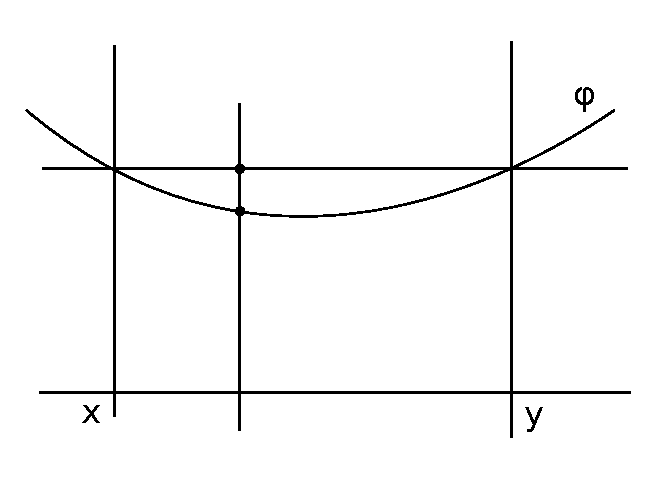
\includegraphics{img/18_lspace_definition.pdf}
      \caption{L-Space definition}
    \end{center}
  \end{figure}
  Graph of $\varphi$ is below the secant between $x$ and $y$.
\end{definition}

\begin{remark}[Exercise]
  \[ \varphi \text{ is convex } \iff \forall a < s < t < u < b \]
  \[ \frac{\varphi(t) - \varphi(s)}{t - s} \leq \frac{\varphi(u) - \varphi(t)}{u - t} \]
  The left-hand side represents the slope of the secant between $s$ and $t$.
  The right-hand side represents the slope of the secant between $t$ and $u$.

  \begin{proposition}
    Let $\varphi$ be convex on $(a, b)$. Then $\varphi$ is continuous on $(a,b)$.
  \end{proposition}
  \begin{proof}[Informal proof sketch]
    $x \in (a,b)$, $y \to x$ ($y > x)$.
    Let $s < x < y < t$.
    $X$ is below $SY$. $Y$ is above the line $SX$. $Y$ is below the line $XT$.

    TODO drawing
  \end{proof}
\end{remark}

\begin{theorem}[Jensen's inequality] % Theorem 4
  Johann Jensen (1859-1925)

  Let ($X, \mathcal A, \mu$) be a probability space (i.e. ($X, \mathcal A, \mu$) is a measure space with $\mu(X) = 1$).
  Let $f \in \mathcal L^1(X)$ and $a < f(x) < b$ for all $x \in X$.
  $a = -\infty$, $b = \infty$ is possible. Moreover, let $\varphi: (a,b) \to \mathbb R$ be convex.
  Then
  \[ \varphi\left(\int_X f \, d\mu\right) \leq \int_X \varphi \circ f \, d\mu \]
\end{theorem}

\begin{proof}
  Let $t = \int_X f \, d\mu$
  \[ a = a \int_X 1 \, d\mu = \int_X a \, d\mu < \int_X f \, d\mu < b \]
  $t \in (a,b)$. Choose $a < s < t$ and $t < u < b$. Then,
  \[ \frac{\varphi(t) - \varphi(s)}{t - s} \leq \frac{\varphi(u) - \varphi(t)}{u-t} \]
  \[ \beta = \sup\setdef{\frac{\varphi(t) - \varphi(s)}{t - s}}{a < s < t} < \infty \]
  We get,
  \[
    \frac{\varphi(t) - \varphi(s)}{t - s} \overbrace{\leq}^{\text{supremum}} \beta
    \iff \varphi(t) \leq \beta(t-s) + \varphi(s)
    \iff \varphi(t) + \beta(s - t) \leq \varphi(s)
    \forall s \in (a,t)
  \]
  For $u > t$,
  \[ \frac{\varphi(u) - \varphi(t)}{u - t} \geq \beta \iff \varphi(u) \geq \varphi(t) + \beta(u - t) \]
  So $\forall y \in (a,b): \varphi(y) \geq \varphi(t) + \beta(y - t)$.
  $y \in (a,t)$ and $y \in (t,b)$.
  Because $f(x) \in (a,b) \implies \varphi(f(x)) > \varphi(t) + \beta(f(x) - t)$.
  \[ \varphi(f(x)) - \varphi(t) - \beta(f(x) - t) \geq 0 \]
  $\varphi$ is continuous. $\varphi \circ f$ is measurable. Integrate:
  \[ \int_X \varphi \circ f \, d\mu - \int_X \varphi(t) \, d\mu - \beta \left(\int_X f \, d\mu - \int_X t \, d\mu\right) \geq 0 \]
  Recognize that $\int_X t \, d\mu = t \int_X 1 \, d\mu = \int_X f \, d\mu$. Furthermore,
  \[ \left(\int_X f \, d\mu - \int_X t \, d\mu\right) = 0 \]
  \[ \int_X \varphi(t) \, d\mu = \varphi(t) \cdot \int_X 1 \, d\mu = \varphi(\int_X f \, d\mu) \]
  Hence,
  \[ \implies \int_X \varphi \circ f \, d\mu \geq \varphi(\int_X f \, d\mu) \]
\end{proof}

\begin{example}
  \[ \varphi(x) = e^x = \exp(x) \]
  \[ \exp(\int_X f \, d\mu) \leq \int_X \exp(f) \, d\mu \]
  \[ X = \set{p_1, p_2, \ldots, p_n} \qquad \mu(\set{p_i}) = \frac{1}{n} \qquad \mu \]
  \[ f(p_i) = x_i \qquad \varphi\left(\frac1n \sum_{i=1}^n x_i\right) \leq \frac{1}{n} \sum_{i=1}^{n} \varphi(x_i) \]
  \[ \varphi = \exp \implies \exp(\frac{1}{n} \sum_{i=1}^n x_i) \leq \frac1n \sum_{i=1}^n e^{x_i} \]

  TODO something is missing here
\end{example}

\dateref{2017/12/13}

\[ \varphi(x) = e^x = \exp(x) \implies \exp\left(\int_X f \, d\mu\right) \leq \int_X \exp(f) \, d\mu \]
$X = \set{p_1, p_2, \ldots, p_n}$ is finite, $\mu(\set{p_i}) = \frac1n$ for $i=1,\ldots,n$.
\[ f: X \to \mathbb R, f(p_i) = X_i \]
\[ \int_X f \, d\mu = \sum_{i=1}^n \underbrace{f(p_i)}_{= x_i} \cdot \underbrace{\mu(\set{p_1})}_{= \frac1n} = \frac1n \sum_{i=1}^n x_i \]
\[ \int_x \exp \circ f \, d\mu = \sum_{i=1}^n e^{x_i} \cdot \frac1n \]

From Jensen's inequality, it follows,
\[ \implies \underbrace{\exp\left(\frac1n \sum_{i=1}^n x_i\right)}_{\left(\exp(\sum_{i=1}^n x_i)\right)^{\frac1n} = \left(\prod_{i=1}^n e^{x_i}\right)^{\frac1n}} \leq \frac1n \sum_{i=1}^n e^{x_i} \]
Let $y_i = e^{x_i} > 0$.
\[ \left(\prod_{i=1}^n y_i\right)^{\frac1n} \leq \frac1n \sum_{i=1}^n y_i \]
Is the inequality of arithmetic and geometric mean.
In some way, Jensen's inequality can be considered as generalization of it.

\index{Conjugate exponents}
\begin{definition}
  Let $p,q > 1$ and suppose $p+q = p\cdot q \iff \frac1q + \frac1p = 1$ then $p$ and $q$ are called \emph{conjugate exponents} (or \emph{pair of conjugate exponents}).
  
  \textbf{Special case:} $p=q=2$ (Hilbert space). \\
  \textbf{Special case} (or actually a definition): We also consider $\frac11 + \frac1\infty = \frac11 + 0 = 1$ so also $(1,\infty)$ is a pair of conjugate exponents.
\end{definition}

\begin{theorem}
  Let $p,q \in (1,\infty)$ be conjugate exponents.
  \index{H\"older's inequality}
  Let $f,g \in \mathcal M_+$ and let $f(x) < \infty$ and $g(x) < \infty$ almost everywhere on $X$. Then H\"older's inequality holds:
  \begin{align}
    \int_X f \cdot g \, d\mu &\leq \left(\int_X f^p \, d\mu\right)^{\frac1p} \left(\int_X g^q \, d\mu\right)^{\frac1q} \label{eq:holder} \\
    \left(\int_X (f + g)^p \, d\mu\right)^{\frac1p} &\leq \left(\int_X f^p \, d\mu\right)^{\frac1p} + \left(\int_X g^p \, d\mu\right)^{\frac1p} \label{eq:minkowski}
  \end{align}
  \index{Minkowsky inequality}
  Equality~\ref{eq:holder} is called H\"older inequality. Equality~\ref{eq:minkowski} is called Minkowski inequality.
  Correspondingly,
  \begin{align*}
    \norm{fg}_{L^1} &\leq \norm{f}_{L^p} \cdot \norm{g}_{L^q}   & f \in L^p(x), g \in L^q(x) \\
    \norm{f+g}_{L^p} &\leq \norm{f}_{L^p} + \norm{g}_{L^p}      & f,g \in L^p(x)
  \end{align*}
\end{theorem}

\begin{proof}
  First, we prove H\"older's inequality.

  Let $A = \left(\int_X f^p \, d\mu\right)^{\frac1p}$ and $B = \left(\int_X g^q \, d\mu\right)^{\frac1q}$.
  \begin{align*}
    A = 0 &\implies \underbrace{f^p}_{\geq 0} = 0 \text{ almost everywhere on } X \\
          &\implies f = 0 \text{ almost everywhere on } X \\
          &\implies \int_X f g \, d\mu = 0 \text{ and right-hand side also } 0
  \end{align*}
  $B = 0 \checkmark$. $A = \infty, B \neq 0 \implies \text{right-hand side} = +\infty \checkmark$. \\
  $A = \infty, B = 0 \implies g = 0$ almost everywhere on $X \implies f \cdot g = 0$ almost everywhere on $X$.
  \[ \implies \int_X fg \, d\mu = 0 \]

  Suppose $A > 0$ and $B > 0$. Let $F = \frac{f}{A}$ and $G = \frac{g}{B}$. Then $\int_x F^p \, d\mu = \frac{1}{A^p} \int_X f^p \, d\mu = 1$.
  \[ \int_X G^q \, d\mu = \frac{1}{B^q} \int_X g^q \, d\mu = 1 \]
  Assume (without loss of generality) $G(x) < \infty, F(x) < \infty$.

  \begin{description}
    \item[Case 1] 
      Let $x \in X$ be such that $G(x) > 0$, $F(x) > 0$. Then there exists $s,t \in \mathbb R$ such that $F(x) = e^{\frac{s}{p}}$ and $G(x) = e^{\frac{t}{q}}$ ($s = \log(F(x)^p)$).
      \[ F(x) G(x) = e^{\frac sp + \frac tq} \underbrace{\leq}_{(*)} \frac1p e^s + \frac1q e^t = \frac1p F(x)^p + \frac1q G(x)^q \]
      where ($*$) follows from the convexity of exponents with $\lambda = \frac{1}{q}$, $1 - \lambda = \frac{1}{p}$.
    \item[Case 2]
      $F(x) = 0$ or $G(x) = 0$.
      \[ \implies F(x) \cdot G(x) = 0 \leq \frac1p F(x)^p + \frac1g G(x)^q \]
      Integration:
      \[ \int_X FG \, d\mu \leq \frac1p \underbrace{\int_X F^p \, d\mu}_{=1} + \frac1q \underbrace{\int_X G^q \, d\mu}_{=1} = \frac1p + \frac1q = 1 \]
      \[ \frac{1}{AB} \int_X fg \, d\mu \leq 1 \implies \int_X fg \, d\mu \leq A \cdot B \checkmark \]
  \end{description}

  Next, we prove the Minkowski inequality.

  Let $p \in (1, \infty)$ given and $q = (1 - \frac1p)^{-1} = \frac{p}{p-1}$. Then $p$ and $q$ are conjugate exponents.
  \[ (f + g)^p = (f + g)(f + g)^{p-1} = f(f+ g)^{p-1} + g(f + g)^{p-1} \]
  By H\"older's inequality,
  \[ \implies \int_X f(f+g)^{p-1} \, d\mu \leq \left(\int_X f^p d\mu\right)^{\frac1p} \cdot \left(\int_X (f + g)^{(pq - q)} \, d\mu\right)^{\frac1q} = \left(\int_X f^p \, d\mu\right)^{\frac1p} \cdot \left(\int_X (f + g)^p \, d\mu\right)^{\frac1q} \]
  \[ \int_X g(f + g)^{p-1} \, d\mu \leq \left(\int_X g^p \, d\mu\right)^{\frac1p} \cdot \left(\int_X (f + g)^p \, d\mu\right)^{\frac1q} \]
  By the sum,
  \[
    \implies \int_X (f + g) (f + g)^{p-1} \, d\mu
    \leq \left[\left(\int_X f^p \, d\mu\right)^{\frac1p} + \left(\int_X g^p \, d\mu\right)^{\frac1p}\right] \left(\int_X (f + g)^p \, d\mu\right)^{\frac1q}
  \]
  \[ \iff \left(\int_X (f + g)^p \, d\mu\right)^{\underbrace{1 - \frac1q}_{=\frac1p}} \leq \left(\int_X f^p \, d\mu\right)^{\frac1p} + \left(\int_X g^p \, d\mu\right) \frac1p \]
\end{proof}

TODO remark is missing

\begin{definition}
  $L^1(X) \checkmark$. let $p \in (q, \infty)$. We set
  \[ L^p(X) = \setdef{f \in \mathcal M}{\int_X \card{f}^p \, d\mu < \infty} \]
  and we set,
  \[ L^p(X) = \setdef{\overline{f}}{f \in L^p(X)} \]
  where $\overline{f}$ is the equivalence class of $f$ with respect to equality almost everywhere.

  For $f \in \mathcal L^p(X)$ we set $\norm{f}_{L^p} = \norm{f}_p = \left(\int_X \card{f}^p \, d\mu\right)^{\frac1p}$.
  For $\overline{f} \in \mathcal L^1(X)$ we set $\norm{f}_{L^p} = \norm{f}_p \coloneqq \norm{f}_p$ for any $f \in \overline{f}$.
  Notation $\norm{f}_{L^p}$ instead of $\norm{\overline{f}}_{L^p}$.
\end{definition}

\begin{remark}
  $\norm{\cdot}_{L^p}$ is a norm on $L^p(X)$.
  \begin{itemize}
    \item $\norm{\overline{f}}_{L^p} = 0 \iff \left(\int_X \card{f}^p \, d\mu\right)^{\frac1p} = 0 \iff \card{f}^p = 0 \text{ almost everywhere on X } \iff \overline{f} = \overline{0}$.
    \item Triangle inequality $\iff$ Morkowski inequality.
    \item $\norm{\lambda f}_{L^p} = \left(\int_X \card{\lambda}^p \card{f}^p \, d\mu\right)^{\frac1p} = \left(\card{\lambda}^p \int_X \card{f}^p \, d\mu\right)^{\frac1p} = \card{\lambda} \norm{f}_{L^p}$
  \end{itemize}
\end{remark}

\index{Banach space}
\begin{theorem}
  Let $1 \leq p < \infty$. Then $L^p(X)$ is a complete normed space, i.e. every Cauchy sequence $(f_n)_{n \in \mathbb N}$ in $L^p(X)$ has a limit $f \in L^p(X)$. $L^p(X)$ is called a \emph{Banach space}.
\end{theorem}
\begin{proof}
  Let $(f_n)_{n \in \mathbb N}$ be a Cauchy sequence in $L^p(X)$, i.e. $\norm{f_n - f_m} < \varepsilon$ if $m,n$ are sufficiently large.
  We choose a subsequence $(f_{n_i})_{i \in \mathbb N}$ such that $\norm{f_{n_{i+1}} - f_{n_{i}}} < \frac{1}{2^i}$.
  For $k \in \mathbb N$, we let $g_k(x) = \sum_{i=1}^k \card{f_{n_{i+1}}(x) - f_{n_i}(x)}$ and $g(x) \coloneqq \sum_{i=1}^\infty \card{f_{n_{i+1}} - f_{n_{i}}(x)} \in [0,\infty]$. We have $g = \lim_{k\to\infty} g_k$ pointwise on $X$. By Minkowski's inequality,
  \[ \card{g_k}_p \leq \sum_{i=1}^k \norm{f_{n_{i+1}} - f_{n_i}}_p < \sum_{i=1}^k \frac{1}{2^i} < 1 \]
  By Fatou,
  \[ \int_X g^p \, d\mu = \int_X \lim_{k\to\infty} g_k^p \, d\mu \leq \liminf_{k\to\infty} \int_X g_k^p \, d\mu \leq \int_X \liminf_{k\to\infty} g_k^p \, d\mu \leq 1 \] % TODO: verify this line

  \[ \int_X g^p \, d\mu < \infty \implies g^p(x) < \infty \text{ almost everywhere on } X \implies g(x) < \infty \text{almost everywhere on } X \]
  \[ g(x) = \sum_{i=1}^{\infty} \card{f_{n_{i+1}}(x) - f_{n_i}(x)}  < \infty \text{ almost everywhere on } X \]
  Consider,
  \[ f(x) = f_{n_i}(x) + \sum_{i=1}^{\infty} \left(f_{n_{i+1}}(x) - f_{n_i}(x)\right) \]
  where the sum is absolutely convergent almost everywhere on $X$ due to $\sum_{i=1}^{\infty} \card{f_{n_{i+1}}(x) - f_{n_i}(x)}  < \infty$ a.e. on $X$.
  We define,
  \[
    f(x) \coloneqq \begin{cases}
      f_{n_i}(x) + \sum_{i=1}^\infty \left(f_{n_{i+1}}(x) - f_{n_i}(x)\right) & \text{if the series converges absolutely} \\
      0 & \text{otherwise}
    \end{cases}
  \]
  We have
  \[ f_{n_{k+1}} = f_{n_i} + \sum_{i=1}^k \left(f_{n_{i+1}} - f_{n_i}\right) \to f \text{ almost everywhere on } X \]

  Show: $\norm{f - f_n}_p \to 0$ as $n \to \infty$.

  Choose $\varepsilon > 0$ and $N \in \mathbb N$ such that $n,m \geq N \implies \norm{f_n - f_m} < \varepsilon$. Fatou:
  \begin{align*}
    \int_X \card{f - f_n}^p \, d\mu &= \int_X \card{\lim_{i\to\infty} f_{n_i} - f_n} \, d\mu \\
      &\leq \liminf_{i\to\infty} \int_X \card{f_{n_i} - f_n}^p \, d\mu = \liminf_{i\to\infty} \underbrace{\norm{f_{n_i} - f_n}_p^p}_{< \varepsilon} \text{ for } n_i \geq N
  \end{align*}
  So $\int_X \card{f - f_n}^p \, d\mu \leq \varepsilon^p$ if $n \geq N$. $\implies \norm{f - f_n}_{L^p} \to 0$ as $n \to \infty$.

  The last remaining argument: Show that $f \in L^p(X)$.

  By Minkowsky's inequality, 
  \begin{align*}
    \left(\int_X \card{f}^p \, d\mu\right)^{\frac1p} &= \left(\int_X \card{f - f_n + f_n}^p \, d\mu\right)^{\frac1p} \\
      &\leq \left(\underbrace{\int_X \card{f_n - f}^p \, d\mu}_{<1 \text{ if $n$ is sufficiently large}}\right)^{\frac1p} + \left(\underbrace{\int_X \card{f_n}^p \, d\mu}_{<\infty}\right)^{\frac1p} < \infty
  \end{align*}
\end{proof}

\begin{corollary}
  Let $f_n \to f$ in $L^p$ where $(f_n)_{n \in \mathbb N}$ is also a Cauchy sequence.
  Then there exists a subsequence $(f_{n_i})_{i \in \mathbb N}$ such that $f_{n_i}(x) \to f(x)$ almost everywhere on $X$.
\end{corollary}

\dateref{2017/12/15}

$L^p(X)$ is a complete normed vector space (Banach space) for every $1 \leq p \leq \infty$, $l(\alpha x + \beta y) = \alpha l(x) + \beta l(y)$.

\begin{definition}
  Let $B$ be a Banach space over $\mathbb R$. A linear map $l: B \to \mathbb R$ with the property $\exists C \geq 0$ s.t. $\card{l(x)} \leq C \norm{x} \forall x \in B$.
  $l$ is called a bounded linear functional on $B$.
  We set $B^* = \setdef{l}{l \text{ is bounded linear functional on $B$}}$.
  Then $B^*$ is a vector space and $\norm{l}_{B^*} = \inf\setdef{c \geq 0}{\card{l(x)} \leq c \norm{x} \forall x \in X}$ is a norm on $B^*$.
  $B^*$ is also a Banach space. We call $B^*$ the dual space to $B$.
\end{definition}

Consider conjugate exponents $p,q \in (1,\infty)$ and fix $g \in L^q(X)$. Consider $l(f) = \int_X f \cdot g \, d\mu$ for $f \in L^p(X)$. Then $l$ is linear on $L^p(X)$.
\[ \card{l(f)} = \card{\int_X f \cdot g \, d\mu} \leq \int_X \card{f \cdot g} \, d\mu \underbrace{\leq}_{\text{H\"older}} \norm{g}_{L^q} \card{f}_{L^p} = C \norm{f}_{L^p} \]
with $C = \norm{g}_{L^q}$. So $l \in \left(L^p(X)\right)^*$. It holds that
\begin{itemize}
  \item $\norm{l}_{(L^p)^*} = \norm{g}_{L^q}$
  \item $\forall l \in (L^p(X))^*$ there exists $g \in L^q(X)$ such that $l(f) = \int_X f \cdot g \, d\mu$.
\end{itemize}
We say $\left(L^p(X)\right)^* = L^q(X)$.

\begin{definition}
  Let $g \in \mathcal M_+$. Let $\alpha \in \mathbb R$ such that $\mu(g^{-1}((\alpha, \beta])) = 0$. $S = \setdef{\alpha \geq 0}{\mu(g^{-1}((\alpha, \infty])) = 0}$.
  If $S \neq \emptyset$, we set $\beta = \inf S$. We say that $g$ is essentially bounded from above if $S \neq \emptyset$ and we call $\beta$ the \emph{smallest essential upper bound for $g$} or \emph{essential supremum of $g$}.
\end{definition}

\[ \alpha \in S \iff g(x) \leq \alpha \text{ almost everywhere on } X \]
We have $\beta \in S$, i.e. \enquote{inf} = \enquote{min}.
\[ \underbrace{g^{-1}((\beta, \infty])}_{\text{nullset}} = \bigcup_{n=1}^\infty \underbrace{g^{-1}\left(\left(\beta + \frac1n, \infty\right]\right)}_{\text{nullset}} \]

$\beta = \operatorname{esssup}(g)$ if $S \neq \emptyset$. $\operatorname{esssup}(g) = \infty$ if $S = \emptyset$.

\begin{definition}
  We set $\mathcal L^\infty(X) = \setdef{f \in \mathcal M}{\operatorname{esssup}\card{f} < \infty}$.
  $\mathcal L^\infty(X)$ is a vector space over $\mathbb R$ (verify!).
  We say that $f \in \mathcal L^\infty(X)$ is essentially bounded.
  We set $\norm{f}_\infty = \operatorname{esssup}\card{f}$.
  Again we define $L^\infty = \setdef{\overline{f}}{f \in \mathcal L^\infty(x)}$.
\end{definition}

Now we what to verify the statement: $\norm{f}_\infty$ is a norm on $L^{\infty}(X)$.

\begin{theorem}
  $L^\infty(X)$ is complete with respect to $\norm{\cdot}_{\infty}$.
\end{theorem}
\begin{proof}
  Let $(f_n)_{n\in\mathbb N}$ is a Cauchy sequence in $L^\infty(X)$.
  \[ A_K = \set{x \in X: \card{f_k(x)} > \norm{f_k}_{\infty}}, \mu(A_k) = 0 \]
  \[ B_{n,m} = \setdef{x \in X: \card{f_n(x) - f_m(x)} > \norm{f_n - f_m}_{\infty}}, \mu(B_{m,n}) = 0 \]
  \[ E = \left(\bigcup_{k=1}^\infty A_k\right) \cup \left(\bigcup_{m,n=1}^\infty B_{n,m}\right) \implies \mu(E) = 0 \]
  Then
  \[ \forall x \in X \setminus E \text{ and } \forall \varepsilon > 0 \exists N \in \mathbb N: m,n > N \implies \card{f_n(x) - f_m(x)} \leq \norm{f_n - f_m}_{\infty} < \varepsilon \]
  The inequality $<$ on the right is given because $(f_n)$ is a Cauchy sequence.
  i.e. $(f_n(x))_{n\in\mathbb N}$ is a Cauchy sequence in $\mathbb R$.
  Completeness of $\mathbb R$: $\exists \alpha_x \in \mathbb R: f_n(x) \to \alpha_x$ as $n \to \infty$.
  We define
  \[ f(x) \coloneqq \begin{cases} \alpha_x & x \in E \\ 0 & x \not\in E \end{cases} \]
  $f_n \to f$ pointwise almost everywhere on $X$. Then $\forall x \in X \setminus E$ and $n \geq N$.
  \[ \card{f_n(x) - f(x)} = \lim_{m\to\infty} \card{\underbrace{f_n(x) - f_m(x)}_{< \varepsilon}} \leq \varepsilon \]
  So, $\norm{f_n - f}_{\infty} < \varepsilon$ if $n \geq N$.
  $f_n \to f$ in $L^\infty(X)$.
  \[ \card{f} \leq \card{f - f_N} + \card{f_N} \leq \varepsilon + \card{f_N} \]
  for $x \in X \setminus E \implies \norm{f}_{\infty} \leq \underbrace{\varepsilon + \norm{f_N}}_{<\infty}$.
\end{proof}

\dateref{2018/01/10}

Does the Fundamental Theorem of Calculus hold?
\[ f(x) = F'(x) \forall x \in [a,b] \]
We will discuss this now. Furthermore, usually we write
\[ \int_a^b f(x) \, dx = F(b) - F(a) \]
In case of Lebesgue integral, we write instead
\[ \int_{[a,b]} f \, d\lambda \]

\[ \lambda(\mathbb R^2) \quad E = [\alpha, \beta] \times [\gamma, \delta] \]
\begin{figure}[!h]
  \begin{center}
    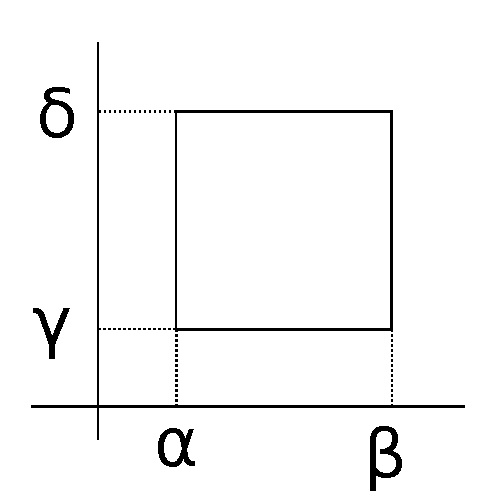
\includegraphics{img/19_E.pdf}
    \caption{$E$}
    \label{img:19E}
  \end{center}
\end{figure}
\[ f: E \to \mathbb R \]
\[ \int_E f \, d\lambda = \int_{[\alpha, \beta] \times [\gamma, \delta]} f(x,y) \, dx \, dy = \int_{y=\gamma}^{\delta} \underbrace{\int_{x=\alpha}^\beta f(x,y) \, dx}_{g(y)} \, dy \]
Compare with Figure~\ref{img:19E}.

\begin{theorem}[Transformation theorem] % Theorem 8
  Set $\mathcal S_b = \setdef{s \in \mathcal S}{\mu(\setdef{x \in X}{s(x) \neq 0}) < \infty}$ where $\mathcal S$ stands for \emph{simple}.
  Then $\mathcal S_b$ is dense in $L^p(X)$ for all $1 \leq p \leq \infty$.
\end{theorem}

\subsection{Product measure and Fubini's Theorem}
Fubini's theorem is a wonderful tool to simplify proofs.

\begin{definition}[Dynkin class, Dynkin system\footnote{In German, \enquote{Dynkin \emph{System}} is used exclusively}]
  Let $X$ be a set. A subset $D \subseteq P(X)$ is called a Dynkin class (d-system), if
  \begin{enumerate}
    \item $X \in D$
    \item $\forall A,B \in D: B \subseteq A \implies A \setminus B \in D$
    \item $\forall A_n \in D: A_n \subseteq A_{n+1}, \forall n \in \mathbb N: \bigcup_{n=1}^\infty A_n \in D$
  \end{enumerate}
  So the definition is similar to a sigma algebra, but condition 3 is different.
  Often it is easier to prove that a set is a Dynkin system, compared to a sigma algebra.
  $\mathcal C' \subseteq P(X)$ is called a $\pi$-system if $\forall A, B \in \mathcal C', A \cap B \in \mathcal C'$.
\end{definition}

Let $\mathcal C \subseteq P(X)$. We call $D_{\mathcal C} \coloneqq \bigcap_{\substack{\mathcal C \subseteq D \\ D \text{ is } d\text{-system}}} D$ a $d$-system (the smallest Dynkin system containing $\mathcal C$).
$D_{\mathcal C}$ is a $d$-system generated by $\mathcal C$.
\[ \mathcal C \subseteq P(X): A_{\mathcal C} = \bigcap_{\substack{\mathcal C \subseteq A \\ A \text{ is } \sigma\text{-algebra}}} A \]

\begin{theorem} % Theorem 1
  \label{thm:one}
  Let $X$ be a set, $\mathcal C \subseteq P(X)$ be a $\pi$-system. Then $D_{\mathcal C} = A_{\mathcal C}$.
\end{theorem}
\begin{proof}
  Every $\sigma$-algebra is a $d$-system $\implies D_{\mathcal C} \subseteq A_{\mathcal C}$.

  \textbf{Show:} $A_{\mathcal C} \subseteq D_{\mathcal C}$ by proving that $D_{\mathcal C}$ is itself a $\sigma$-algebra.

  We start by showing $A,B \in D_{\mathcal C} \implies A \cap B \in D_{\mathcal C}$.
  \[ D_1 = \setdef{A \in D_{\mathcal C}}{A \cap C \in D_C \forall C \in \mathcal C} \]
  if $C' \in \mathcal C \implies C' \cap C \in \mathcal C \subseteq D_{\mathcal C} \forall C \in \mathcal C$ because $\mathcal C$ is a $\pi$-system.
  \[ \implies \mathcal C \subseteq D_1 \]

  \textbf{Show:} $D_1$ is a $d$-class,
  \[ X \cap C = C \in \mathcal C \subseteq D_{\mathcal C} \forall C \in \mathcal C \]
  \[ \implies X \in D_1 \checkmark \]
  First property is proven.

  Let $A,B \in D_1$ with $B \subseteq A$. Then $(A \setminus B) \cap C = \underbrace{(A \cap C)}_{\in D_{\mathcal C}} \setminus \underbrace{(B \cap C)}_{\in D_{\mathcal C}} \in D_{\mathcal C} \qquad \forall C \in \mathcal C$
  because $D_{\mathcal C}$ is a $d$-system.
  \[ \implies A \setminus B \in D_1 \]
  Second property is proven.

  Let $A_n \in D_1, A_n \subseteq A_{n+1} \forall n \in \mathbb N$.
  \[ (\bigcup_{n=1}^\infty A_n) \cap C = \bigcup_{n=1}^\infty \left(\overbrace{\underbrace{A_n \cap C}_{\in D_C}}^{(A_n \cap C) \subseteq (A_{n+1} \cap C)}\right) \in D_{\mathcal C} \implies \bigcup_{n=1}^\infty A_n \in D_1 \]
  So $D_1$ is a d-system which contains $\mathcal C \implies D_{\mathcal C} \subseteq D_1$, $D_1 \subseteq D_{\mathcal C}$ by definition $\implies D_1 = D_{\mathcal C}$.
  For all $A \in D_{\mathcal C}$ and for all $C \in \mathcal C: A \cap C \in D_{\mathcal C}$.

  \[ D_2 = \setdef{B \in D_{\mathcal C}}{A \cap B \in D_{\mathcal C} \forall A \in D_{\mathcal C}} \]
  by first step: $\mathcal C \subseteq D_2: D_2$ is a $d$-system. Proof as in step 1 for $D_1$.
  \[ \implies D_{\mathcal C} \subseteq D_2 \text{ and } D_2 \subseteq D_{\mathcal C} \text{ by definition } \implies D_2 = D_{\mathcal C} \]
  \[ \forall A, B \in D_{\mathcal C}: A \cap B \in D_{\mathcal C} \]
  Use this, to show that $D_{\mathcal C}$ is a $\sigma$-algebra.
  Let $A \in D_{\mathcal C}, X \in D_{\mathcal C} \implies A^C = X \setminus A \in D_{\mathcal C}$ by the second property.
  Let $A_n \in D_{\mathcal C}$ for $n \in \mathbb N$. Show that $\bigcup_{k=1}^n A_k \in D_{\mathcal C} \forall n \in \mathbb N$.

  \[ \bigcup_{k=1}^n A_k = \left(\left(\bigcup_{k=1}^n A_k\right)^C\right)^C = \left(\bigcap_{k=1}^n \underbrace{A_k^C}_{\in D_{\mathcal C}}\right)^C \in D_{\mathcal C} \]
  because $D_{\mathcal C}$ is closed with respect to finite intersection.
  So $D_{\mathcal C}$ is an algebra.
  We let $B_1 = A_1$ and $B_n = A_n \setminus \left(\bigcup_{k=1}^{n-1} A_k\right)$.
  \[ B_n = \bigcup_{k=1}^n A_n \in D_{\mathcal C}, B_n \subseteq B_{n+1} \text{ and } \bigcup_{n=1}^\infty A_n = \bigcup_{n=1}^\infty B_n \in D_{\mathcal C} \text{ due to property 3} \]
  \[ \implies \bigcup_{n=1}^\infty A_n \in D_{\mathcal C} \forall A_n \in D_{\mathcal C} \]
  $\implies D_{\mathcal C}$ is a $\sigma$-algebra and hence $D_{\mathcal C} \subseteq A_{\mathcal C}$.
\end{proof}

\begin{corollary}
  Let $X$ be a set, $A$ be a $\sigma$-algebra on $X$, $\mathcal C$ is a $\pi$-system on $X$.
  $A = A_{\mathcal C}$. Let $\mu, \nu$ be measures on $\mathcal A$, $\mu(X) < \infty$ and $\nu(X) < \infty$ (finite measures).
  Suppose $\nu(C) = \nu(C) \forall C \in \mathcal C$ and $\mu(X) = \nu(X)$. Then $\nu(A) = \mu(A) \forall A \in \mathcal A$.
\end{corollary}
\begin{proof}
  Let $D = \setdef{A \in \mathcal A}{\mu(A) = \nu(A)}, C \in D \forall C \in \mathcal C \implies \mathcal C \subseteq D$.
  Show that $D$ is a d-system. $X \in D$ because $\nu(X) = \mu(X)$.
  Let $A, B \in D: B \subseteq A$. Then $B \cup (A \setminus B) = A \implies \mu(B) + \mu(A \setminus B) = \mu(A)$ and 
  $\nu(B) + \nu(A \setminus B) = \nu(A)$. In both LHS expressions, the set is finite. Hence, the RHS is finite correspondingly.
  \[ \implies \mu(A \setminus B) = \underbrace{\mu(A)}_{\in D} - \underbrace{\mu(B)}_{\in D} = \mu(A) - \mu(B) = \mu(A \setminus B) \]
  \[ \implies A \setminus B \in D \]
  Let $A_n \in D, A_n \subseteq A_{n+1} \forall n \in \mathbb N$.
  Then
  \[ \mu\left(\bigcup_{n=1}^\infty A_n\right) = \lim_{n\to\infty} \mu(A_n) \underbrace{=}_{\text{because } A_n \in D} \lim_{n\to\infty} \nu(A_n) = \nu(\bigcup_{n=1}^\infty A_n) \]
  $D$ is a $d$-system and (remember ($D_{\mathcal C} = A_{\mathcal C}$ by Theorem~\ref{thm:one})) $D_{\mathcal C} \subset D \implies A = A_{\mathcal C} \subseteq D \subseteq A$ with $A_n \in D$.
  $\implies D = A$, so $\forall A \in \mathcal A: \mu(A) = \nu(A)$.
\end{proof}

\begin{corollary}
  Let $A$ be a $\sigma$-algebra on $X$, $\mathcal C$ be a $\pi$-system on $X$.
  $\mathcal A = \mathcal A_{\mathcal C}$. Let $\mu, \nu$ be measures on $\mathcal A$ wich coincide on $\mathcal C$ ($\nu(C) = \mu(C) \forall c \in \mathcal C$)
  and assume that $(C_n)_{n \in \mathbb N}$ exists with $C_n \in \mathcal C$, $C_n \subseteq C_{n+1}$, $X = \bigcup_{n=1}^\infty C_n$ and $\nu(C_n) < \infty$,
  $\mu(C_n) < \infty$ for all $n \in \mathbb N$. Then $\nu = \mu$ on $\mathcal A$.
\end{corollary}
\begin{definition}
  Let $(X, \mathcal A)$ and $(Y, \mathcal B)$ be sets with $\sigma$-algebras $\mathcal A$ and $\mathcal B$ respectively.
  We consider $Z = X \times Y$. We call a set $C = A \times B \subseteq X \times Y$ with $A \in \mathcal A$ and $B \in \mathcal B$
  a measurable rectangle in $X \times Y$.

  $A \times B$ is the product $\sigma$-algebra of $A$ and $B$.
  Let $C = \setdef{A \times B}{A \in \mathcal A, B \in \mathcal B} \subseteq P(X \times Y)$. Then we set $A \times B = A_{\mathcal C}$ is a
  $\sigma$-algebra in $X \times Y$ generated by the measurable rectangles.
\end{definition}
\begin{figure}[!h]
  \begin{center}
    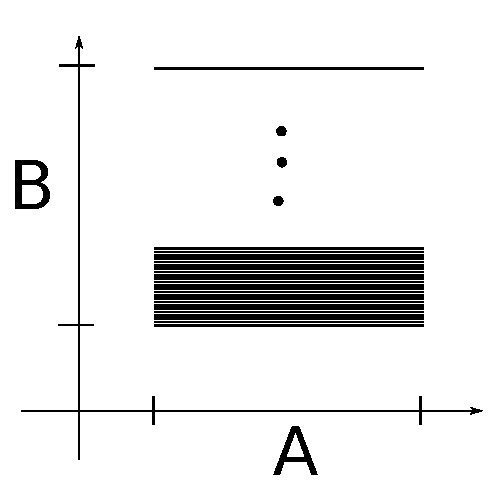
\includegraphics{img/20_area.pdf}
    \caption{Area as the cartesian product of lines}
    \label{img:area}
  \end{center}
  \begin{center}
    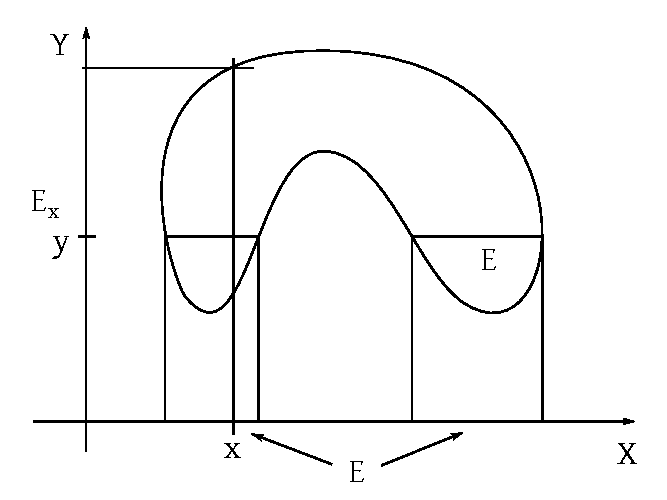
\includegraphics{img/20_5_sections.pdf}
    \caption{$E$}
    \label{img:205}
  \end{center}
\end{figure}
\begin{remark}
  $\mathcal C$ is a $\pi$-system: $A$, $A' \in \mathcal A$ and $B, B' \in \mathcal B$.
  \begin{align*}
    (A \times B) \cap (A' \times B')(
          &= \setdef{(a, b) \in X \times Y}{a \in A \cap A' \land b \in B \cap B'} \\
          &= \underbrace{(A \cap A')}_{\in \mathcal A} \times \underbrace{(B \cap B')}_{\in \mathcal B} \in \mathcal C
  \end{align*}
\end{remark}
\begin{definition}
  $A, B, X, Y$ as above.
  $E \subseteq X \times Y$. We set $E_X = \setdef{y \in Y: (x, y) \in E} \subseteq Y$ for some given $x \in X$.
  \[ E^Y = \setdef{x \in X}{(x, y) \in E} \subseteq X \]
  for some given $y \in Y$.
  $E_x, E^y$ are called \emph{sections of $E$}.
\end{definition}

\dateref{2018/01/12}

\[ E \subseteq X \times Y \qquad E_x = \setdef{y \in Y}{(x, y) \in E} \qquad E^y = \setdef{x \in X}{(x, y) \in E} \]
\[ \pi_x: X \times Y \to X \qquad \pi_x((x, y)) = x \]
\[ \pi_y: X \times Y \to Y \qquad \pi^y((x, y)) = y \]
Suppose $f: X \times Y \to Z$. For $x \in X$ fixed, we set $f_x: Y \to Z$, $f_x(Y) = f(x, y)$.
For $y \in Y$ fixed, $f^y: X \to Z$, $f^y(x) = f(x, y)$ (compare with Figure~\ref{img:E}).

\begin{figure}[!h]
  \begin{center}
    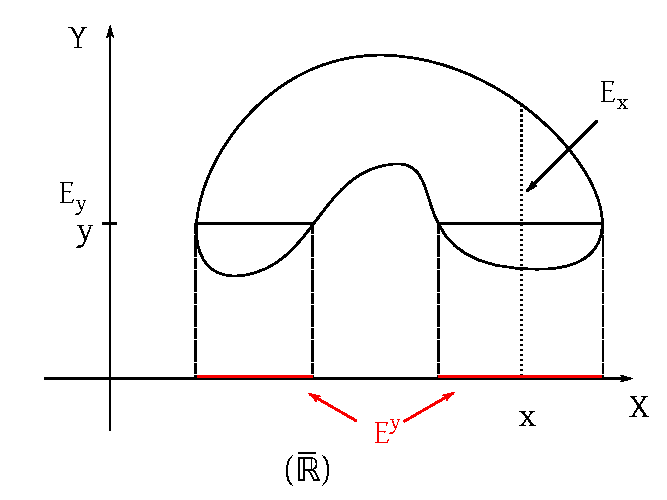
\includegraphics{img/21_Ex_Ey.pdf}
    \caption{$E_x$, $E^x$ and $E^y$}
    \label{img:E}
  \end{center}
\end{figure}

$\mathcal A \times \mathcal B \subseteq P(X \times Y)$. $\mathcal A \times \mathcal B$ is the $\sigma$-algebra generated by all measurable rectangles
$\mathcal A \times \mathcal B$, $A \in \mathcal A$, $B \in \mathcal B$, $\mathcal C = \setdef{A \times B}{A \in \mathcal A, B \in \mathcal B}$ is a $\pi$-system.

\begin{lemma} % Lemma 1
  Let $X, Y$ be sets, $\mathcal A$ is a $\sigma$-algebra on $X$, $\mathcal B$ is a $\sigma$-algebra on $Y$, $\mathcal A \times \mathcal B$ as above. Then
  \begin{enumerate}
    \item For any $E \subset \mathcal A \times \mathcal B$, any $x \in X$ and any $y \in Y$, we have $E_x \in \mathcal B$, $E^y \in \mathcal A$.
    \item Let $f: X \times Y \to \overline{\mathbb R}$ be measurable with respect to $\mathcal A \times \mathcal B$.
      Then for any $x \in X$ and $y \in Y$ the function $f_x$ is $\mathcal B$-measurable and $f^y$ is $\mathcal A$-measurable.
  \end{enumerate}
\end{lemma}
\begin{proof}
  \begin{enumerate}
    \item Let $\mathcal F = \setdef{E \subset X \times Y}{E_x \in \mathcal B \forall x \in X}$. Show $\mathcal A \times \mathcal B \subseteq \mathcal F$
      by $\mathcal C \subseteq \mathcal F$ and $\mathcal F$ is a $\sigma$-algebra. $\mathcal F$ is a $\sigma$-algebra, because
      \begin{enumerate}
        \item $\emptyset \in \mathcal F$ because $\emptyset_x = \emptyset \in \mathcal B \forall x \in X$
        \item $X \times Y \in \mathcal F$ because $(X \times Y)_x = Y \in \mathcal B \forall x \in X$
      \end{enumerate}
      Let $E \in \mathcal F$.
      \[ (E^C)_x = \setdef{y \in Y}{(x, y) \not\in E} = \setdef{y \in Y}{y \not\in E_x} = (E_x)^C \in \mathcal B \]
      where $E_x \in \mathcal B$ because $E \in \mathcal F$.
      $(E_n)_{n \in \mathbb N}$ for $E_n \in \mathcal F \forall n \in \mathbb N$.
      \[ \left(\bigcup_{n=1}^\infty E_n\right)_x = \setdef{y \in Y}{\exists n \in \mathbb N: (x,y) \in E_n} = \bigcup_{n=1}^\infty \setdef{y \in Y}{(x,y) \in E_n} \]
      Therefore $\mathcal F$ is a $\sigma$-algebra (compare with Figure~\ref{img:rectAB}).
      \begin{figure}[!h]
        \begin{center}
          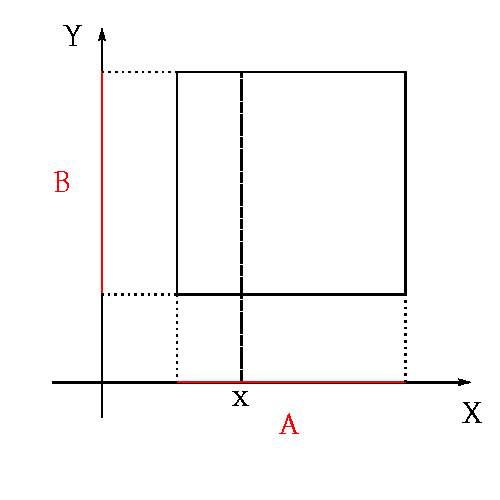
\includegraphics{img/22.pdf}
          \caption{Rectangle $A \times B$}
          \label{img:rectAB}
        \end{center}
      \end{figure}

      Show $\mathcal C \subseteq \mathcal F$: Let $E = A \times B$. Then
      \[ E_x = \setdef{y \in Y}{(x, y) \in A \times b} = \begin{cases} B & \text{if } x \in A \\ \emptyset & \text{if } x \not\in A \end{cases} \]
      so $A \times B \in \mathcal F$ and $\mathcal C \subseteq \mathcal F \implies \mathcal A \times \mathcal B \subseteq \mathcal F$.

      The same argument holds true for $E^y$.

    \item Show $f_x: Y \to \overline{\mathbb R}$ is measurable with respect to $\mathcal B$. Let $\alpha \in \mathbb R$.
      \[ f_x^{-1}([\alpha, \infty]) = \setdef{y \in Y}{\underbrace{f_x(y)}_{=f(x,y)} \in [\alpha, \infty]} = \left[f^{-1}([\alpha, \infty])\right]_x \in \mathcal B \]
      where $f^{-1}([\alpha, \infty]) \in \mathcal A \times \mathcal B$ because $f$ is measurable with respect to $\mathcal A \times \mathcal B$.

      The same argument holds true for $f^y$.
  \end{enumerate}
\end{proof}

Let $(X, \mathcal A, \mu)$ be a measure space. We say that $(X, \mathcal A, \mu)$ is $\sigma$-finite if there exists
$(A_n)_{n \in \mathbb N}, A_n \in \mathcal A, A_n \cap A_m = \emptyset$ for $n \neq m$, $\mu(A_n) < \infty$ and $\bigcup_{n=1}^\infty A_n = X$.

Set $C_n = \bigcup_{k=1}^n A_n$ then $\mu(C_n) = \sum_{k=1}^n \mu(A_k) < \infty$.
$C_n \subseteq C_{n+1}, \bigcup_{n=1}^\infty C_n = \bigcup_{n=1}^\infty A_n = X$.

\begin{proposition} % Proposition 1
  Let $(X, \mathcal A, \mu)$ and $(Y, \mathcal B, \nu)$ be finite measure spaces. Then for any $E \in \mathcal A \times \mathcal B$ the map
  \[ f_E: X \to [0,\infty] \qquad f_E(x) = \nu(E_x) \quad (x \mapsto \nu(E_x)) \]
  is $\mathcal A$-measurable. Likewise,
  \[ g_E: Y \to [0,\infty] \qquad g_E(y) = \mu(E^y) \]
  is $\mathcal B$-measurable.
\end{proposition}
\begin{proof}
  First case: $\nu(Y) < \infty$.

  \[ \mathcal F = \setdef{E \subseteq X \times Y}{x \to \nu(E_x) \text{ is } \mathcal A\text{-measurable}} \]
  \begin{figure}[!h]
    \begin{center}
      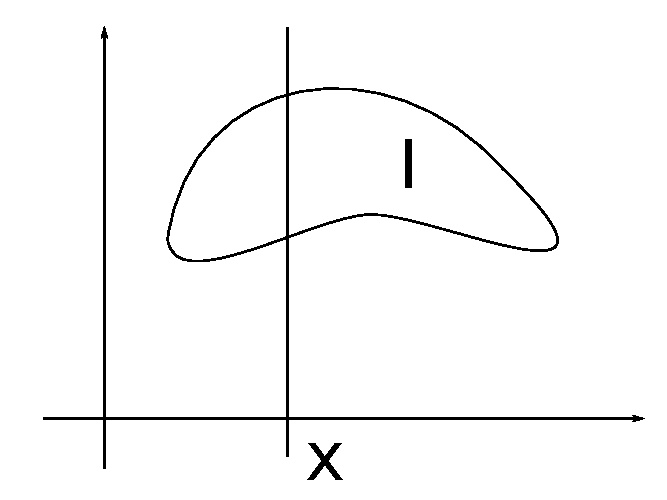
\includegraphics{img/23_I.pdf}
      \caption{$I$}
      \label{img:23i}
    \end{center}
  \end{figure}

  \textbf{Show:} $\mathcal C \subseteq \mathcal F$ and $\mathcal F$ is a $d$-system.
  Let $E = A \times B \in \mathcal C$ and
  \[
    x \mapsto \nu(E_x) = \begin{cases}
      \nu(B) & \text{ for } x \in A \\
      \nu(\emptyset) = 0 & \text{ for } x \not\in A
    \end{cases}
  \]
  so $f_E = \nu(B) \chi_A \in \mathcal A$ where $\nu(B) < \infty$ because $\nu(Y) < \infty$ so $\mathcal C \subseteq \mathcal F$.

  $d$-system:
  \[ \nu(\emptyset_X) = 0 \forall x \in X \text{ and } x \mapsto 0 \text{ is measurable} \]
  Let $F \subseteq E$ and $F, E \in \mathcal F: E \setminus F \in \mathcal F$.
  Show this membership.
  \begin{align*}
    (E \setminus F)_X &= \setdef{y \in Y}{(x, y) \in E \text{ and } (x,y) \not\in F} \\
      &= \setdef{y \in Y}{(x, y) \in E} \setminus \setdef{y \in Y}{(x, y) \in F} \\
      &= E_x \setminus F_x \\
    \nu((E \setminus F)_X) &= \nu(E_x \setminus F_x) = \underbrace{\nu(E_x)}_{<\infty} - \underbrace{\nu(F_x)}_{<\infty}
  \end{align*}
  $x \mapsto \nu((E \setminus F)_x)$ is the difference of two measurable functions, hence it is measurable.

  \dateref{2018/01/17}

  Revision: We have the following setting: $E \in \mathcal A \times \mathcal B$.
  $x \mapsto \nu(E_x)$ is $\mathcal A$-measurable. $X \to [0, \infty]$.

  \textbf{Assumption:} $\nu(Y) < \infty$.

  \[ \mathcal F = \setdef{E \subseteq X \times Y}{x \to \nu(E_x) \text{ is measurable}} \]
  \[ \mathcal C = \setdef{A \times B}{A \in \mathcal A, B \in \mathcal B} \subseteq \mathcal F \]
  \[ \emptyset \in \mathcal F, E,F \in \mathcal F \text{ with } F \subseteq E \implies E \setminus F \in \mathcal F \]
  Let $E_n \in F$, $E_n \subseteq E_{n+1}$. Show $\bigcup_{n=1}^\infty E_n \in \mathcal F$.

  \[ \left(\bigcup_{n=1}^\infty E_n\right)_X = \setdef{y \in Y}{(x, y) \in E_n \text{ for one } n \in \mathbb N} = \bigcup_{n=1}^\infty (E_n)_x \]
  \[ (E_n)_x \subseteq (E_{n+1})_x \]
  \[ \nu\left(\bigcup_{n+1}^\infty (E_n)_x\right) = \lim_{n\to\infty} \nu((E_n)_x) \]
  \[ x \mapsto \nu\left(\left(\bigcup_{n=1}^\infty E_n\right)_x\right) = \lim_{n\to\infty} \nu((E_n)_x) \]
  measurable as limit of measurable function.
  So $\mathcal F$ is a $d$-system, $\mathcal C \subseteq \mathcal F$, $\mathcal C$ is a $\pi$-system.
  \[ \xRightarrow{\text{by Theorem~\ref{thm:one}}} \mathcal A \times \mathcal B \subseteq \mathcal F \]

  \textbf{Case 2:} Let $D_n \in \mathcal B$ with $\nu(D_n) < \infty$.

  $D_n \cap D_m = \emptyset$ if $n \neq m$ and $Y = \bigcup_{n=1}^\infty D_n$ (i.e. $Y$ is $\sigma$-finite).
  We define $\nu_n: \mathcal B \to [0, \infty)$.
  \[ \nu_n(B) = \nu(D_n \cap B) \]
  $\nu_n$ is a measure on $\mathcal B$.
  \[ \nu_n(B) \leq \nu_n(Y) = \nu(D_n) < \infty \]
  \[
    \forall B \in \mathcal B: \nu(B) = \nu\left(\underbrace{\left(\bigcup_{n=1}^\infty D_n\right)}_{=Y} \cap B\right)
    = \nu\left(\bigcup_{n=1}^\infty \left(D_n \cap B\right)\right)
    = \sum_{n=1}^\infty \nu\left(D_n \cap B\right)
    = \sum_{n=1}^\infty \nu_n(B)
  \]
  $x \mapsto \nu_n(E_x)$ is measurable by part 1 for all $n \in \mathbb N$ and $E \in \mathcal A \times \mathcal B$.
  $x \mapsto \nu(E_x) = \sum_{n=1}^\infty \nu_n(E_x)$ is measurable as sum of measurable non-negative functions.
\end{proof}

\begin{theorem}  % Theorem 2
  \label{thm:two}
  Let $(X, \mathcal A, \mu)$, $(Y, \mathcal B, \nu)$ be a $\sigma$-finite measure spaces. Then there exists a unique measure $\mu \times \nu$ on $\mathcal A \times \mathcal B$ such that
  $\forall A \times B \in \mathcal C$ we have $(\mu \times \nu)(A \times B) = \mu(A) \cdot \mu(B)$. Moreover, we have
  \[ (\mu \times \nu)(E) = \int_X \nu(E_x) \, d\mu = \int_Y \mu(E^y) \, d\nu  \qquad \forall E \in \mathcal A \times \mathcal B \]
  $\mu \times \nu$ is called the produce measure.

  Compare with Figure~\ref{img:24}.
\end{theorem}
\begin{figure}[!h]
  \begin{center}
    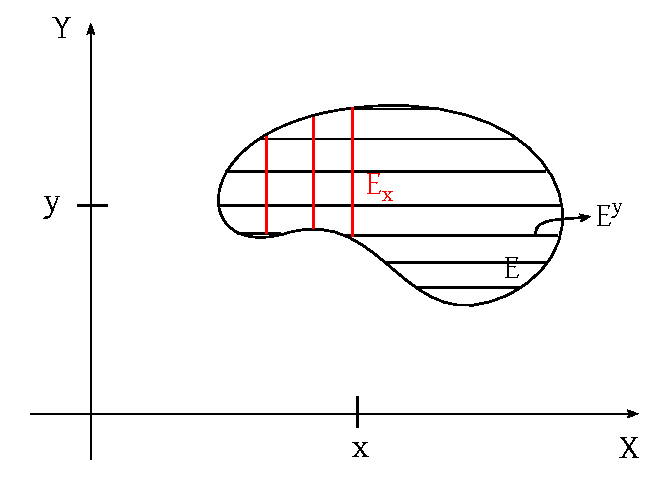
\includegraphics{img/24.pdf}
    \caption{Setting for Theorem~\ref{thm:two}}
    \label{img:24}  \end{center}
\end{figure}
\begin{proof}
  $x \mapsto \nu(E_x)$ is non-negative, $m$-able $\forall E \in \mathcal A \times \mathcal B$.
  $y \mapsto \mu(E^y)$ is non-negative, $m$-able $\forall E \in \mathcal A \times \mathcal B$.
  So $\int_Y \nu(E_x) \, d\mu \eqqcolon (\mu \times \nu)_1 (E)$, $\int_Y \mu(E^Y) \, d\nu \eqqcolon (\mu \times \nu)_2 (E)$.

  Check: $(\nu \times \nu)_1$ and $(\mu \times \nu)_2$ are both measures on $\mathcal A \times \mathcal B$ (exercise).

  \textbf{Case 1:} $\mu(X) < \infty$ and $\nu(Y) < \infty \implies (\mu \times \nu)_1$ and $(\mu \times \nu)_2$ are finite.
  Let $E = A \times B \in \mathcal C$. Then $(\mu \times \nu)_1 (E) = \int_X \underbrace{\nu(E_x)}_{\nu(B) \chi_A} \, d\mu = \nu(B) \cdot \int_X \chi_A \, d\mu = \nu(B) \mu(A)$ and $(\mu \times \nu)_2(E) = \int_Y \mu(E^y) \, d\mu = \int_y \mu(A) \chi_B \, d\nu = \mu(A) \nu(B)$.
  So $\forall E \in \mathcal C: (\mu \times \nu)_1 (E) = (\mu \times \nu)_2(E)$.
  \[ F = \setdef{E \in \mathcal A \times \mathcal B}{(\mu \times \nu)_1 (E) = (\mu \times \nu)_2 (E)} \]
  Show that $\mathcal F$ is a $d$-systemm, $\emptyset \in \mathcal F$.

  \[ (\mu \times \nu)_1(F) = (\mu \times \nu)_2(F) \]
  Let $E, F \in \mathcal F, F \subseteq E$.
  \begin{align*}
    (\mu \times \nu)_1 (F) + (\mu \times \nu)_1 (E \setminus F) &= \\
    (\mu \times \nu)_1 (E) = (\mu \times \nu)_2 (E) &= \\
    (\mu \times \nu)_2 (F) + (\mu \times \nu)_2 (E \setminus F) &
  \end{align*}

  We get $(\mu \times \nu)_1 (E \setminus F) = (\mu \times \nu)_2 (E \setminus F)$.
  Let $E_n \in \mathcal F, E_n \subseteq E_{n+1}, \mtn_1(E_n) = \lim_{n\to\infty}\mtn_1(E_n) = \lim_{n\to\infty}\mtn_2(E_n) = \mtn_2(\bigcup_{n=1}^\infty E_n)$.
  So $\mathcal F$ is a $d$-system.

  By Theorem~\ref{thm:one}, $\mathcal A \times \mathcal B \subseteq \mathcal F \subseteq \mathcal A \times \mathcal B$.
  So $\forall E \in \mathcal A \times \mathcal B: (\mu \times \nu_1)(E) = (\mu \times \nu)_2(E)$.
  So also any measure $\kappa$ on $\mathcal A \times \mathcal B$ which coincides with $\mtn_1$ on $\mathcal C$ also coincides with $\mtn_1$ on $\mathcal A \times \mathcal B \implies$ uniqueness.

  \textbf{Case 2:} $\sigma$-finite mesaures:
  \[ A_n \in \mathcal A \qquad X = \bigcup_{n=1}^\infty A_n \qquad \mu(A_n) < \infty \qquad A_n \subseteq A_{n+1} \]  % ascending
  $B_n \in \mathcal B$, $Y = \bigcup_{n=1}^\infty B_n$, $\nu(B_n) < \infty$, $C_n = A_n \times B_n,
  \mtn_1(C_n) = \mu(A_n) \nu(B_n) = \mtn_2(C_n) < \infty$. $\mtn_1(E) = \mtn_1(E \cap \bigcup_{n=1}^\infty C_n) = \lim_{n\to\infty} \mtn_1 (E \cap C_n)$.
  $= \lim_{n\to\infty} \mtn_2 (E \cap C_n)$ by part 1, $=\mtn_2(E)$.
\end{proof}

Leonida Tonelli, 1885--1946

\begin{theorem}[Tonelli's Theorem]
  Let $(X, \mathcal A, \mu)$, $(Y, \mathcal B, \nu)$ be $\sigma$-finite measure spaces.
  Let $f: X \times Y \to [0, \infty]$ be $\mathcal A \times \mathcal B$ measurable. Then,
  \begin{enumerate}
    \item $x \mapsto \int_y f_x \, dy$ is $\mu$-measurable. $y \mapsto \int_x f^y \, d\mu$ is $\mathcal B$-measurable.
    \item $\int_X \left( \int_y f_x \, d\nu\right) d\mu = \int_Y \left(\int_X f^y \, d\mu\right) \, d\nu = \int_{X \times Y} f \, d(\mu \times \nu)$.
  \end{enumerate}
\end{theorem}
\begin{remark}
  $f_x(y) = f(x, y)$ and $f^y(x) = f(x,y)$.
  \[ \int_X \int_Y f(x,y) \, d\nu(y) \, d\mu(x) = \int_Y \int_X f(x,y) \, d\mu(x) \, d\nu(y) \]
\end{remark}
\begin{proof}
  We know $y \mapsto f_x(y)$ is non-negative and $\nu$-measurable so $\int_y f_x\, d\nu$ exists.
  Likewise: $\int_X f^y \, d\mu$ exists $\forall y \in Y$.
  We start with $f = \chi_E$ with $E \in \mathcal A \times \mathcal B$.
  Then, \[ (\chi_E)_x(y) = \begin{cases} 1 & \underbrace{(x,y)}_{\Leftrightarrow y \in E_X} \in E \\ 0 & \text{else} \end{cases} \]
  and this equals $\chi_{E_x}(y)$, so  $\int_Y(\chi_E)_X\,d\nu = \int_Y \chi_{E_x} \, d\nu = \nu(E_x)$. Therefore,
  \[ \int_X \int_Y (\chi_E)_x \, d\nu \, d\mu = \int_Y \nu(E_x) \,d\mu \]
  Analogously:
  \[ \int_Y \int_X (\chi_E)^Y \, d\mu \, d\nu = \int_Y \mu(E^y) \, d\nu \]
  but $\int_Y \nu(E_x) \,d\mu = \int_Y \mu(E^y) \, d\nu$ by Theorem~\ref{thm:two}.
  \[ \stackrel{\text{by def.}}{=} \mtn(E) = \int_{X\times Y} \chi_E d\mtn \]
  So the two statement of this theorem hold for all characteristic functions $\chi_E$ for $E \in \mathcal A \times \mathcal B$.
  This implies that both statements hold for linear combinations of characteristic functions, i.e. for simple functions.

  Let $f$ be $\mathcal A \times \mathcal B$ be measurable, $f: X \times Y \to [0, \infty]$. Then
  $f = \lim_{n\to\infty} S_n$ pointwise $s_n \leq s_{n+1}$.
  \[ \int_{X\times Y} f d\mtn \stackrel{\substack{\text{by monotone} \\ \text{convergence} \\ \text{theorem}}}{=} \lim_{n\to\infty} s_n d \mtn = \lim_{n\to\infty} \int_X \underbrace{\int_Y \underbrace{(S_n)_x}_{\text{measurable}} \, d\nu}_{\text{measurable}} \, d\mu \]
  \[ \stackrel{\substack{\text{by monotone} \\ \text{convergence} \\ \text{theorem}}}{=} \int_X \int_Y \underbrace{\lim_{n\to\infty} (S_n)_X}_{=f_x} \, d\nu \, d\mu = \int_X \int_Y f_x \, d\nu \, d\mu \]
  Then we can do a symmetric argument:
  \[ \int_{X \times Y} f \, d(\mu \times \nu) = \int_Y \int_X f^Y \, d\mu \, d\nu \]
\end{proof}

\dateref{2018/01/19}

Let
\[ f: X \times Y \to [0, \infty] \]
be $\mathcal A \times \mathcal B$ measurable.
\[ \int_{X \times Y} f \, d(\mtn) = \int_X \int_Y f_x \, d\nu \, d\mu = \int_Y \int_X f^Y \, d\mu \, d\nu \]

Guido Fubini (1876--1943)

\begin{theorem}[Fubini's Theorem] % Theorem four
  \label{thm:four}
  Let $(X, \mathcal A, \mu)$, $(Y, \mathcal B, \nu)$ be $\sigma$-finite measure spaces.
  Let $f: X \times Y = \overline{\mathbb R}$ be $\mtn$-integrable (i.e., $\int_X \card{f} \, d\mtn < \infty$).
  Then:
  \begin{enumerate}
    \item for $\mu$ almost every $x \in X$ the section $f_X: Y \to \overline{\mathbb R}$ is $\nu$-integrable
      and for $\nu$ almost every $y \in Y$ the section $f_Y: X \to \overline{\mathbb R}$ is $\mu$-integrable.
    \item The functions
      \[ I_f(x) = \begin{cases} \int_Y f_X \, d\nu & \text{if } f_X \text{ is integrable} \\ 0 & \text{ else} \end{cases} \]
      \[ I_f(y) = \begin{cases} \int_X f^Y \, d\mu & \text{if } f^Y \text{ is integrable} \\ 0 & \text{ else} \end{cases} \]
      are integrable with respect to $\mu$ and $\nu$ respectively.
    \item And
      \[ \int_X I_f(x) \, d\mu = \int_X I_f(y) \, d\nu = \int_{X \times Y} f \, d\mtn \]
  \end{enumerate}
\end{theorem}
\begin{proof}
  We will only prove the statements for $X$, the statement for $Y$ follow by symmetry.
  \[ f = f^+ - f^- \text{ and } \card{f} = f^+ + f^- \]
  $f_X^+$, $f_X^-$, $f_x$ are measurable.
  By Tonelli's theorem it follows that
  \[ x \mapsto \int_X f_X^+ \, d\mu \]
  \[ x \mapsto \int_Y f_X^+ \, d\nu \]
  are measurable with respect to $\mathcal A$. By Tonelli's Law,
  \[ \infty > \int_{X \times Y} \card{f} \, d\mtn \geq \int_{X\times Y} f^+ \, d\mtn = \int_X \int_Y f_X^+ \, d\nu \, d\mu \]
  \[ \implies \int_Y f_X^+ \, d\nu < \infty \text{ for almost every } x \in X \]
  By the same argument, $\int_Y f_X^- \, d\nu < \infty$ for almost every $x \in X$.
  \[ N = \setdef{x \in X}{\int_Y f_X^+ \, d\nu = \infty \text{ or } \int_X f_X^- \, d\nu = \infty} \]
  then $\mu(N) = 0$. Almost everywhere on $X$:
  \[ \int_Y \card{f_X} \, d\nu < \infty \]
  \[ \int_Y \card{f_X} \, d\nu = \underbrace{\int_Y f_X^+ \, d\nu}_{<\infty} + \underbrace{\int_Y f_X^- \, d\nu}_{<\infty} \]
  for $x \in X \setminus N$.

  Define $I_f(x)$ as in the second statement,
  \begin{align*}
    \int_{X\times Y} f \, d\mtn
      &= f^+ \, d\mtn + \int_{X\times Y} f^- \, d\mtn \\
      &\stackrel{\text{by Tonelli}}= \int_X \int_Y f_X^+ \, d\nu \, d\mu - \int_X \int_Y f^-_X \, d\nu \, d\mu \\
      &= \int_{X \setminus N} \underbrace{\int_Y (f_X^+ - f_X^-)}_{=I_f(x)} \, d\nu \, d\mu \\
      &= \int_X I_f(x) \, d\mu
  \end{align*}
  Hence, we proved the third statement.

  We use the same argument for $\card{f}$ instead of $f$.
  \begin{align*}
    \int_{X\times Y} \card{f} \, d\mtn
      &= \int_{X\times Y} \left(f_X^+ + f_X^-\right) \, d\mtn \\
      &= \int_X \int_Y f_X^+ \, d\nu \, d\mu + \int_X \int_Y f_X^- \, d\nu \, d\mu \\
      &= \int_{X\setminus N} \underbrace{\int_Y \left(f_X^+ + f_X^-\right) \, d\nu}_{\int_Y \card{f_X} \, d\nu > \card{\int_Y f_X \, d\nu} = \card{I_f}(x) \text{ for } x \in X \setminus N} \, d\mu
  \end{align*}
  \[ \implies \int_X \card{I_f(x)} \, d\mu < \infty \]
  which proves the second statement.
\end{proof}

\[ \mathbb R^{k+l} = \mathbb R^k + \mathbb R^l \]
\[ \int_{\mathbb R^{k+l}} f \, d \lambda^{k+l} = \int_{\mathbb R^k} \int_{\mathbb R^l} f_X \, d\lambda^l \, d\lambda^k \]

\index{Borel $\sigma$-algebra}
$\mathcal B^k \subseteq \mathcal P(\mathbb R^k)$ is called \enquote{Borel $\sigma$-algebra on $\mathbb R^k$}.
The $\sigma$-algebra generated by all half open $k$-dimensional parallelograms $\mathcal W = \set{\bigtimes_{i=1}^k [\alpha_i, \beta_i): \alpha_i \leq \beta_i}$.
$\mathcal B^k \subseteq \mathcal L^k$. $\mathcal W$ is a $\pi$-system.
Consider product $\sigma$-algebra $\mathcal B^k \times \mathcal B^l$ on $\mathbb R^k \times \mathbb R^l = \mathbb R^{k+l}$ and $\mathcal B^{k+l}$ on $\mathbb R^{k+l}$. It holds that $\mathcal B^k \times \mathcal B^l = \mathcal B^{k+l}$. Let $R \in \mathcal W^k \subseteq \mathcal B^k$ and $S \in \mathcal W^l \subseteq \mathcal B^l$ be given. Then $R \times S \in \mathcal W^{k+l}$. $\mathcal B^{k+l}$ is generated by $R \times S \in \mathcal W^{k+l}$. $R \times S$ is a measurable rectangle in $\mathcal B^k \times \mathcal B^l$, so $\mathcal B^k \times \mathcal B^l$ is a $\sigma$-algebra which contains $\mathcal W^{k+l} \implies \mathcal B^k \times \mathcal B^l \supseteq \mathcal B^{k+l}$.
\dateref{2018/01/24}

\[ \mathcal B^k \times \mathcal B^l = \mathcal B^{k + l} \]
with $\mathcal B^k \times \mathcal B^l \supseteq \mathcal W^k \times \mathcal W^l = \mathcal W^{k + l}$ and $\mathcal B^{k + l}$ generated by $\mathcal W^{k + l}$
\[ \mathcal B^{k+l} \subseteq \mathcal B^k \times \mathcal B^l \]

\[ \pi_k: \mathbb R^{k+l} \to \mathbb R^k \qquad \pi_l: \mathbb R^{k+l} \to \mathbb R^l \]
\[
  \pi_k \begin{bmatrix} x_1 \\ \vdots \\ x_k \\ y_1 \\ \vdots \\ y_l \end{bmatrix} = \begin{bmatrix} x_1 \\ \vdots \\ x_k \end{bmatrix} \qquad
  \pi_l \begin{bmatrix} x_1 \\ \vdots \\ x_k \\ y_1 \\ \vdots \\ y_l \end{bmatrix} = \begin{bmatrix} y_1 \\ \vdots \\ y_k \end{bmatrix}
\]

$\pi_k$, $\pi_l$ are linear hence continuous, hence Borel measurable.
Let $A \subseteq \mathcal B^k$, $\pi_k^{-1}(A) = A \times \mathbb R^l \in \mathcal B^{k + l}$.
\[ \pi_l^{-1}(B) = \mathbb R^k \times B \in \mathcal B^{k + l} \forall B \in \mathcal B^l \]
\[ A \times B = (A \times \mathbb R^l) \cap (\mathbb R^k \times B) \in \mathcal B^{k+l} \]
where $A \times B$ is a measurable rectangle generate $\mathcal B^k \times \mathcal B^l$.
\[ \implies \mathcal B^k \times \mathcal B^l \subseteq \mathcal B^{k+l} \]
QED.

Caution: $\mathcal L^k \times \mathcal L^l \neq \mathcal L^{k+l}$.
Choose $A \subseteq \mathbb R^k$, $A \not\in \mathcal L^k$. $0 \in \mathbb R^l$, $A' = A \times \set{0} \subseteq \mathbb R^{k+l}$
with $A \times \set{0} \subseteq \mathbb R^k \times \set{0}$ satisfies $\lambda^{k+l}(\mathbb R^k \times \set{0}) = 0$.
$A \times \set{0}$ is a nullset in $\mathbb R^{k+l}$, $A \times \set{0} \in \mathcal L^{k+l}$
but $A'^0 = (A \times \set{0})^0 = A \not\in \mathcal L^k$ where $A'^0$ denotes a section with $y=0$.
So $A \times \set{0} \not\in \mathcal L^k \times \mathcal L^l$ because otherwise the section would need to lie in $\mathcal L^k$.

\begin{lemma}
  $\forall A \in \mathcal B^k, B \in \mathcal B^l:$ we have $A \times B \subseteq \mathcal B^{k+l} \subseteq \mathcal L^{k + l}$
  and $\lambda^{k+l}(A \times B) = \lambda(A) \lambda(B)$.
\end{lemma}
\begin{proof}
  $W^k$ and $W^l$ are $\pi$-systems. For $R \in W^k, S \in W^l \implies R \times S \in W^{k+l}$ and $\lambda^{k+l}(R \times S) = \lambda^k(R) \times \lambda^l(S)$
  (where equality is given by definition of $\lambda^{k+l}$ for elements in $W$).
  \[ \mathcal F_1 = \setdef{A \in \mathcal B^k}{\lambda^{k+l}(A \times S) = \lambda^k(A) \cdot \lambda(S) \forall S \in W^l} \]
  Then $W^k \subseteq \mathcal F_1$. You can check that $\mathcal F_1$ is indeed a $d$-system.
  So $\mathcal F_1$ contains $\mathcal B^k$. So $\forall A \in \mathcal B^k$ and $\forall S \in W^l$ we have $\lambda^{k+l}(A \times S) = \lambda^k(A) \cdot \lambda^l(S)$.
  \[ \mathcal F_2 = \setdef{B \in \mathcal B^l}{\lambda ^{k+l}(A \times B) = \lambda^k(A) \lambda^l(B) \forall A \in \mathcal B^k} \]
  $W^l \subseteq \mathcal F_2$ and $\mathcal F_2$ is a $d$-system (check yourself).
  \[ \implies \mathcal F_2 \supseteq \mathcal B^l \]
\end{proof}

Some facts about $\lambda^k$, $\mathcal L^k$:

\begin{theorem}[regularity of $\lambda^k$]
  Let $A \in \mathcal L^k$. Then
  \begin{itemize}
    \item $\lambda(A) = \sup\setdef{\lambda(K)}{K \subseteq A \text{ and } K \text{ is compact}}$
    \item $\lambda(A) = \inf\setdef{\lambda(K)}{A \subseteq U \text{ and } U \text{ is open}}$
  \end{itemize}
\end{theorem}

\begin{theorem}
  $\lambda$ is translation-invariant, i.e., $\lambda(A + v) = \lambda(A)$.
  \[ \forall A \in \mathcal L, v \in \mathbb R^k \]
  Any Borel-measure $\mu: \mathcal B \to [0, \infty]$ which is also translation invariant
  has the property that $\mu(A) = C \cdot \lambda(A) \forall A \in \mathcal B$ with some constant $c \geq 0$.

  This is a special case of the Haar measure for locally compact topological groups.
\end{theorem}

\subsection{Differentiation}

Generalization of $\int_a^b f(u(x)) \cdot u'(x) \, dx = \int_{u(a)}^{u(b)} f(\xi) \, d\xi$.

\begin{proposition}
  Let $T: \mathbb R^k \to \mathbb R^k$ be linear, invertible.
  Then $\forall A \in \mathcal B^k: \lambda(T(A)) = \card{\det(T)} \cdot \lambda(A) \quad \forall A \in \mathcal B^k$.
\end{proposition}
\begin{proof}
  We have for $A \in \mathcal B: T^{-1}(A) \in \mathcal B$ ($T^{-1}$: linear $\implies$ continuous $\implies$ measurable).
  \[ T(A) = (T^{-1})^{-1}(A) \in \mathcal B \qquad \forall A \in \mathcal B \]
  \[ T = T_1 \circ T_2 \circ \ldots \circ T_n \]
  for some $n \in \mathbb N$ and $T_i$ are elementary transformations of the Gaussian algorithm (LU decomposition).
  $T_l$ has one of the following matrix representations:
  \begin{itemize}
    \item \[ \underbrace{T_l = \begin{bmatrix} 1 & & & & 0 \\ & \ddots & & & \\ & & \alpha_1 & & \\ & & & \ddots & \\ 0 & & & & 1 \end{bmatrix}}_{T_{i,\alpha}} \]
    \item \[ \underbrace{T_l = \begin{bmatrix} 1 & & & & & \\ & \ddots & & & & \\ & & 0 & 1 & & \\ & & 1 & 0 & & \\ & & & & \ddots & \\ & & & & & 1 \end{bmatrix}}_{S_{i,j}} \]
      where $01$ is in the $i$-th row and $10$ is in the $j$-th row.
    \item \[ \underbrace{T_l = \begin{bmatrix} 1 & & & & & \\ & \ddots & & & & \\ & & 1 & 1 & & \\ & & & 1 & & \\ & & & & \ddots & \\ & & & & & 1 \end{bmatrix}}_{T_{i,j}} \]
      where $11$ is in the $i$-th row and $1$ is in the $j$-th row.
  \end{itemize}
  Let $B \in W$, $B = \bigtimes_{l=1}^k [\alpha_l, \beta_l)$.
  \[ \lambda(T_{i,\alpha}(B)) = ? \]
  \[ T_{i,a}(B) = \bigtimes_{l=1}^{i-1} [\alpha_l, \beta_l) \times \underbrace{[a \cdot \alpha_i, a \cdot \beta_i)}_{\text{length: } \card{a} (\beta_i - \alpha_i)} \times \bigtimes_{l=i+1}^k [\alpha_l, \beta_l) \]
  \[ \lambda(T_{i,a}(B)) = \card{a} \prod_{l=1}^n (\beta_l - \alpha_l) = \card{a} \cdot \lambda(B) = \card{\det(T_{i,a})} \cdot \lambda(B) \]
  \[ \lambda(S_{i,j}(B)) = \lambda(B) = \underbrace{\card{\underbrace{\det{S_{i,j}}}_{=-1}}}_{=1} \cdot \lambda(B) \]
  \[ \lambda(T_{i,j}(B)) = ? \]
  \[ T_{i,j}(B) = \setdef{\begin{bmatrix} \hat x_1 \\ \vdots \\ \hat x_k \end{bmatrix}}{\hat x_l \in [\alpha_l, \beta_l) \text{ for } l \neq i \text{ and } \hat x_i \in [\alpha_i + \hat x_j, \beta_i + \hat x_j)} \]
  \[ \left(T_{i,j}(B)\right)^{\hat x_j = \text{ const}}, \lambda^{k-1}\left((T_{i,j}(B))^{x_j}\right) = \lambda^{k-1}\underbrace{([\alpha_1, \beta_1) \times \dots \times [\alpha_i + \hat x_j, \beta_i + \hat x_j) \times \dots \times [\alpha_n, \beta_k)}_{\text{no } j\text{-th component}}) \]
  \[ = (\beta_1 - \alpha_1) \dots (\beta_i + \hat x_j - \alpha_i - \hat x_j) \dots (\beta_k - \alpha_k) = (\beta_1 - \alpha_1) \dots \underbrace{(\beta_i - \alpha_i)}_{\text{no } j\text{-th component}} \dots (\beta_k - \alpha_k) \]
  \[ \lambda(T_{i,j}(B)) \stackrel{\text{Fubini}}= \int_{[\alpha_j, \beta_j)} \lambda^{k-1}(T_{i,j}(B)) \, d\lambda^1 = \prod_{\substack{l=1 \\ l \neq j}}^k (\beta_l - \alpha_l) \cdot (\beta_j - \alpha_j) = \lambda(B) = \card{\underbrace{\det(T_{i,j}}_{=1})} \cdot \lambda(B) \]
  So let $T = T_1 \dots T_n, B \in W$. Then
  \[ \lambda(T(B)) = \lambda(T_1 \dots T_n(B)) = \card{\det(T_1)} \cdot \lambda(T_2 \dots T_n(B)) \]
  \[ = \dots \card{\det{T_1}} \cdot \card{\det{T_2}} \cdot \dots \cdot \card{\det{T_n}} \cdot \lambda(B) = \card{\det(T_1 \dots T_n)} \cdot \lambda(B) = \card{\det(T)} \cdot \lambda(B) \]
  Set $\mathcal F = \setdef{A \in \mathcal B}{\lambda(T(A)) = \card{\det(T)} \cdot \lambda(A)}$.
  $W \subseteq \mathcal F$ is a $d$-system $\implies \mathcal B \subseteq \mathcal F \subseteq B$.
  So $\forall B \in \mathcal B: \lambda(T(B)) = \card{\det(T)} \lambda(B)$.
\end{proof}

\begin{remark}
  This lemma also (trivially) holds if $\det(T) = 0$.
\end{remark}

\index{Diffeomorphism}
Consider $F: U \to V$, $U, V \subseteq \mathbb R^k$ open, $F \in \mathcal C^1(U, \mathbb R^k)$, $DF(x) \in \mathbb R^{k\times k}$ is a Jacobian matrix.
Assume $F: U \to V$ is bijective and $F^{-1}$ is also $\mathcal C^1$.
$F$ is a $\mathcal{C}^1$ diffeomorphism from $U$ onto $V$.

\begin{theorem}[Transformation theorem]
  Let $F: U \to V$ be a diffeomorphism. $B \subseteq U, B \in \mathcal B$. Then
  \begin{enumerate}
    \item \[ \lambda(F(B)) = \int_B \underbrace{\card{\det(DF(x))}}_{= J_F(x)} \, d\lambda = \int_B \card{J_F(x)} \, d\lambda \]
    \item For $f: V \to \overline{\mathbb R}$ measurable, we have
      \[ \int_V f \, d\lambda = \int_U f \circ F(x) \card{J_F(x)} \, d\lambda(x) \]
  \end{enumerate}
\end{theorem}

\dateref{2018/01/26}

Let $U, V \subseteq \mathbb R^k$ be open, $F: U \to V$ be a $\mathcal C^1$-diffeomorphism.
\[ B \subseteq U \implies \lambda(F(B)) = \int_B \card{J_F(x)} \, d\lambda \]
$f: V \to \overline{\mathbb R}$ integrable:
\[ \int_V f \, d\lambda = \int_U f \circ F(x) \card{J_F(x)} \, dx \]

\begin{lemma}
  Let $U \subseteq \mathbb R^k$ be open, $G: U \to \mathbb R^k$ be a $\mathcal C^1$-function.
  Let $\varepsilon > 0$, $\overline{C} \subseteq U$, $C \in W$ be a cube with side length $b > 0$.
  $C = \bigtimes_{i=1}^k [\alpha_i, \alpha_i+b)$. Assume that
  \[ \forall x \in \overline {C}: \norm{DG(x) - \underbrace{E}_{k\times k \text{ unit matrix}}} \leq \varepsilon \]
  Then $\lambda^*(G(C)) \leq (1 + \varepsilon)^k \cdot \lambda(C)$.

  Remark: $G$ is diffeomorphism. $\lambda^* \leftrightsquigarrow \lambda$.
\end{lemma}
\begin{proof}
  Let $x_0 = \begin{bmatrix} \alpha_1 + \frac b2 \\ \vdots \\ \alpha_k + \frac b2 \end{bmatrix}$
  be the center of the cube.
  $\overline{W} \subseteq U$ compact then DF is bounded on $\overline{W}$.
  \[ \norm{\operatorname{DF}(x)} \leq M \forall x \in \overline{W} \]
  \[ \norm{F(x_1) - F(x_2)} \leq \max_{\xi \in \overline{W}} \underbrace{\norm{\operatorname{DF}(\xi)}}_{\leq M} \norm{x_1 - x_2} \]
  Let $L \in \mathbb R^{n\times n}$. $\norm{L} = \max\setdef{\norm{Lv}_{{\mathbb R^n}}}{\norm{v}_{\mathbb R^n} = 1}$.
  Then $\norm{Lv}_{\mathbb R^n} \leq \norm{L} \cdot \norm{v}_{\mathbb R^n}$. Use $\norm{\cdot}_\infty$ on $\mathbb R^n$.

  \[ \max\setdef{\card{x_i - x_{0,i}}}{x \in C, i = 1,\ldots,k} < \frac b2 \]
  \[ \implies \norm{x - x_0}_{\infty} \leq \frac b2 \forall x \in C \]
  \[ \norm{(G - \text{id})(x) - (G - \text{id})(x_0)}_{\infty} \leq \max_{\xi \in \overline{C}} \norm{\text{DG}(\xi) - E} \cdot \norm{x - x_0} \]
  by our remark above.
  \[ \leq \varepsilon \norm{x - x_0}_\infty \]

  \[ \norm{G(x) - G(x_0)}_{\infty} \leq \norm{(G - \text{id})(x) - (G - \text{id})(x_0)}_{\infty} + \norm{x - x_0}_{\infty} \]
  \[ \leq (1 + \varepsilon)\norm{x - x_0} \leq (1 + \varepsilon) \frac{b}{2} \]
  \[ G(C) \subseteq \bigtimes_{i=1}^{k} \left[ G(x_0)_i - (1 + \varepsilon) \frac b2, G(x_0)_i + (1 + \varepsilon) \frac b2 \right] \]
  \[ \lambda^*(G(C)) \leq \prod_{i=1}^k (1 + \varepsilon) \cdot b = (1 + \varepsilon)^k \cdot b^k = (1 + \varepsilon)^k \lambda(C) \]
\end{proof}

\begin{lemma}
  Let $U, V, F$ be as in the statement of the transformation theorem.
  Let $a > 0, B \subseteq U, B \in \mathcal B$.
  \begin{itemize}
    \item if $\card{J_F(x)} \leq a \forall x \in B$ then $\lambda(F(B)) \leq a \lambda(B)$
    \item if $\card{J_F(x)} \geq a \forall x \in B$ then $\lambda(F(B)) \geq a \lambda(B)$.
  \end{itemize}
\end{lemma}
\begin{proof}
  Prove the first statement for the special case $B \subseteq U$ is such that $\overline{B} \subseteq U$ and $\overline{B}$ is compact and $B$ is open.
  We assume that $\norm{J_F(x)} \leq a \forall x \in \overline{B}$.
  $x \mapsto \frac{\partial F^i}{\partial x_j}$ is continuous on $B$ so this function is uniformly continuous.
  $F^{-1}: F(\overline{B}) \to B$ is differentiable with $D(F^{-1}) = (DF)^{-1}$ is continuous on $F(\overline{B})$ (compact) so $DF^{-1}$ is bounded on $F(\overline{B})$.
  Let $M \geq 0$ such that $\norm{(DF)^{-1}(y)} \leq M \forall y \in F(\overline{B})$.
  By uniform continuity of $DF$ on $\overline{B} \implies \forall \varepsilon > 0 \exists \delta > 0: \norm{DF(x) - DF(x_0)} \leq \frac{\varepsilon}{M}$ if $\norm{x - x_0} \leq \delta$ and $x, x_0 \in \overline{B}$.

  \[ B = \bigcup_{i=1}^\infty C_i \text{ with } C_i \in W \]
  $C_i$ is a cube with side length $\leq 2\delta$, $C_i \cap C_j = \emptyset$.

  Let $C$ be one of these cubes and $x_0$ its center.
  \[ G(x) = (DF(x_0))^{-1} \cdot F(x) \text{ for } x \in C \]
  \[ DG - E = (DF(x_0))^{-1} DF(x) - (DF(x_0))^{-1} DF(x_0) = (DF(x_0))^{-1} (DF(x) - DF(x_0)) \]
  \[ \norm{DF(x) - E} \leq \norm{(DF(x_0))^{-1}} \cdot \norm{DF(x) - DF(x_0)} \leq M \frac{\varepsilon}{M} = \varepsilon \]
  because $\norm{x - x_0}_{\infty} < \delta$.
  By the previous Lemma,
  \[ \lambda(F(C)) = \lambda(DF(x_0) \cdot G(c)) = \card{J_F(x_0)} \cdot \lambda(G(C)) \]
  where the equality follows from:
  \[ \lambda(F(B)) \leq a (1 + \varepsilon)^k \sum_{i=1}^\infty \lambda (C_i) = a(1 + \varepsilon)^k \]
  By the lemma,
  \[ \leq a (1 + \varepsilon)^k \lambda(c) \]
\end{proof}

\dateref{2017/01/31}

\[ U, V \subseteq \mathbb R^k \text{ open} \]
\[ F: U \to V \text{ diffeomorphism} \]
\[ B \in \mathbb B, B \subseteq U \]
\begin{itemize}
  \item $\lambda(F(B)) = \int_B \card{J_F(x)} \, d\lambda(x)$
  \item $f: V \to \overline{\mathbb R}$ integrable
\end{itemize}
\[ \int_V f \, d\lambda = \int_u f \circ F(x) \card{J_F(x)} \, d\lambda(x) \]

\begin{lemma}
  If $\card{J_F(x)} \leq a$ on $B$ then $\lambda(F(B)) \leq a \cdot \lambda(B)$.
  If $\card{J_F(x)} \geq a$ on $B$ then $\lambda(F(B)) \geq a \cdot \lambda(B)$.
\end{lemma}
\begin{proof}[Proof of the transformation theorem]\hfill{} \\
  \begin{enumerate}
    \item
      Suppose $\lambda(B) \leq \infty$ and for $n \in \mathbb N$, $k \in \mathbb N$, $n \geq 1$, $k \geq 1$.
      \[ B_{n,k} = \setdef{x \in B}{\frac{k-1}{n} \leq \card{J_F(x)} \leq \frac kn} \]
      \[ B = \bigcup_{k=1}^\infty B_{n,k} \qquad B_{n,k} \cap B_{n,l} = \emptyset \text{ if } k \neq l \]
      \begin{lemma}
        \[ \frac{k-1}{n} \cdot \lambda(B_{n,k}) \leq \lambda(F(B_{n,k})) \leq \frac kn \cdot \lambda(B_{n,k}) \]
      \end{lemma}
      Also:
      \[ \frac{k-1}{n} \lambda(B_{n,k}) \leq \int_{B_{n,k}} \card{J_F(x)} \, d\lambda \leq \frac kn \cdot \lambda(B_{n,k}) \]
      \[ \underbrace{\left(\frac{k-1}{n} - \frac kn\right)}_{-\frac1n} \lambda(B_{n,k}) \leq \lambda(F(B_{n,k})) - \int_{B_{n,k}} \card{J_F(x)} \, d\lambda \leq \underbrace{\left(\frac kn - \frac{k-1}{n}\right)}_{= \frac1n} \lambda(B_n, n) \]
      \[ \card{\lambda(F(B_{n,k})) - \int_{B_{n,k}} \card{J_F(x)} \, d\lambda} \leq \frac1n \lambda(B_{n,k}) \]
      \[ \card{\lambda(F(B)) - \int_B \card{J_F(x)} \, d\lambda} = \card{\sum_{k=1}^\infty \lambda(F(B_{n,k})) - \sum_{k=1}^\infty \int_{B_{n,k}} \card{J_F(x) \, dx}} \]
      \[ \leq \sum_{k=1}^\infty \card{\lambda(F(B_{n,k})) - \int_{B_{n,k}} \card{J_F(x)} \, d\lambda} \leq \frac1n \sum_{k=1}^\infty \lambda(B_{n,k}) \leq \frac1n \underbrace{\lambda(B)}_{<\infty} \forall n \in \mathbb N \]
      \[ \implies \card{\lambda(F(B)) - \int_F \card{J_F(x)} \, d\lambda} = 0 \]
      For $\lambda(B) = \infty$. Set $B = \bigcup_{l=1}^\infty B_l$ with $B_l \cap B_{l'} = \emptyset$ if $l \neq l'$ and $\lambda(B_l) < \infty$.
    \item
      For $f = \chi_C$, $C = F(B)$, $B = F^{-1}(C)$, $C \subseteq V \iff B \subseteq U$.
      \[ \int_V \chi_C \, d\lambda = \lambda(F(B)) \underbrace{=}_{\text{by } a} \int_B \card{J_F(x)} \, d\lambda = \int_U \chi_B \card{J_F} \, d\lambda = \int_U \chi_C \circ  F \cdot \card{J_F} \, d\lambda \]
      So (2.) holds for characteristic functions
      $\implies$ (2.) holds for simple functions
      $\implies$ (2.) holds for $f \in \mathcal M^+(V, \lambda)$ (by approximation of monotone convergence)
      $\implies$ (2.) holds for $f$ integrable (by $f = f^+ - f^-$)
  \end{enumerate}
\end{proof}

\begin{definition}
  \index{Signed measures}
  A few words about signed measures:
  Let $\mathcal A$ be a $\sigma$-algebra on $X$, a map $\nu: \mathcal A \to [-\infty, \infty]$ with
  \begin{enumerate}
    \item $\nu(\emptyset) = 0$
    \item $\forall A_n \in \mathcal A, A_n \cap A_m = \emptyset$ we have $\nu(\bigcup_{n=1}^\infty A_n) = \sum_{n=1}^\infty \nu(A_n)$ makes sense.
  \end{enumerate}
  Then $\nu$ is called a \emph{signed measure on ($X, \mathcal A$)}.
\end{definition}

$P \subseteq X$ with $P \in \mathcal A$ is called a positive set for $\nu$ iff $\forall E \subseteq P$ we have $\nu(E) \geq 0$.
$N \subseteq X$, $N \in \mathcal A$ is called a negative set for $\nu$ iff $\forall E \subseteq N: \nu(E) \leq 0$.

Hans Hahn (1879-1834)

\begin{theorem}[Hahn decomposition theorem]
  \index{Hahn decomposition theorem}
  \index{Jordan decomposition}
  Let $(X, \mathcal A)$ be given and $\nu$ is a signed measure on $X$.
  Then there exists $P,N \in \mathcal A$ with $P \cup N = X$, $P \cap N = \emptyset$ such that
  $P$ is a positive set and $N$ is a negative set for $\nu$.
  We set $\nu_+(A) = \nu(P \cap A) \geq 0 \forall A \in \mathcal A$ is a measure.
  $\nu_-(A) = -\nu(N \cap A) \geq 0 \forall A \in \mathcal A$ is also a measure on $X$.

  $\nu = \nu_+ - \nu_-$ is the \emph{Jordan decomposition} of $\nu$.

  At least one measure ($\nu_+$ or $\nu_-$) must be finite.
\end{theorem}

\begin{example}
  \begin{enumerate}
    \item
      Let $\mu_1$ and $\mu_2$ be measures on $X$, one is finite.
      Then $\nu(A) = \mu_1(A) - \mu_2(A)$ is a signed measure.
    \item
      $\nu(A) = \int_A f \, d\mu$ with $\mu$ measure on $\mathcal A$ and $f$ is an integrable function,
      $\nu$ is a finite signed measure.
      \[ P = \setdef{x \in X}{f(x) \geq 0} \qquad N = \setdef{x \in X}{f(x) < \infty} \]
      \[ \nu_+(A) = \int_A f^+ \, d\mu \qquad \nu_-(A) = \int_A f^- \, d\mu \]
  \end{enumerate}
\end{example}

\begin{definition}
  Let $\nu, \mu$ be measures on $\mathcal A$. We say that $\nu$ is absolutely continuous with respect to $\mu$ ($\nu \ll \mu$)
  iff $\forall A \in \mathcal A$ with $\mu(A) = 0$ we have $\mu(A) = 0$.
\end{definition}

\begin{remark}
  \[ \nu \ll \mu \iff \forall \varepsilon > 0 \exists \delta > 0 \text{ such that } \mu(A) < \delta \implies \nu(A) < \varepsilon \]
  ($A \in \mathcal A$)
  Let $C \in \mathcal A$ and $\mu$ be a measure on $\mathcal A$.
  We say that $\mu$ is concentrated on $C$ iff $\forall A \in \mathcal A: \mu(A) = \mu(A \cap C) \iff \mu(B) = 0 \forall B \cap C = \emptyset$.
  We say that $\nu$ is signular with respect to $\mu \iff \nu$ is concentrated on $S \in \mathcal A$ and $\mu(S) = 0$.
\end{remark}

\begin{theorem}[Lebesgue composition theorem]
  Let $\nu$ and $\mu$ be $\sigma$-finite measures on $\mathcal A$.
  Then $\nu = \nu_a + \nu_s$ with $\nu_a \ll \mu$ and $\nu_s$ is singular with respect to $\mu$.
\end{theorem}

\begin{theorem}[Radon–Nikodym theorem]
  Let $\mathcal A$ be a $\sigma$-algebra on $X$. Let $\nu$ and $\mu$ be measures on $\mathcal A$.
  Let $\nu \ll \mu$. Then there exists $g \in M^+(X, \mathcal A)$ such that
  \[ \mu(A) = \int_A g \, d\mu \qquad \forall A \in \mathcal A \]
  Moreover $g$ is uniquely determined by $\nu$ almost everywhere with respect to $\mu$.
  $g$ is called the Radon-Nikodym derivative of $\nu$.
\end{theorem}
\begin{proof}
  We only prove the theorem for $\mu(X) < \infty$ and $\nu(X) < \infty$.
  \[ G = \setdef{f \in \mathcal M^+(X, \mathcal A)}{\int_A f \, d\mu \leq \nu(A) \forall A \in \mathcal A} \]
  $G \neq \emptyset$ because $0 \in G$. Show that $\exists g \in G$ such that $\int_{X} g \, d\mu \geq \int_X f \, d\mu \forall f \in \mathcal G$.

  We need: if $f_1$ and $f_2 \in \mathcal G$ then $f_1 \lor f_2 = \max(f_1, f_2) \in \mathcal G$. Let $A \in \mathcal A$ be given
  \[ A_1 = \setdef{x \in A}{f_1(x) \geq f_2(x)} \in \mathcal A \]
  \[ A_2 = \setdef{x \in A}{f_2(x) > f_1(x)} \in \mathcal A \]
  \[ \int_A(f_1 \lor f_2) \, d\mu = \int_{A_1} f_1 \, d\mu + \int_{A_2} f_2 \, d\mu \overbrace{\leq}^{f_1, f_2 \in \mathcal G} \nu(A_1) + \nu(A_2) = \nu(A) \]
  so $f_1 \lor f_2 \in \mathcal G$.
  $f_n \in \mathcal G$ with $\lim_{n\to\infty} \int_X f_n \, d\mu = S$ without loss of generality by replacing $f_n$ with $f_1 \lor f_2 \lor \ldots \lor f_n$.
  Let $s = \sup\setdef{\int_X f \, d\mu}{f \in \mathcal G}$ and $(f_n)_{n\in\mathbb N}$. We can assume that $f_n \leq f_{n+1}$.

  $f_n \leq f_{n+1}$. $g(x) = \lim_{n\to\infty} f_n(x)$, $g \in \mathcal M^+$ and we have $\lim_{n\to\infty} \int_X f_n \, d\mu = \int_X g \, d\mu$
  by monotone convergence and $\nu(A) \geq \lim_{n\to\infty} f_n \, d\mu = \int_A g \, d\mu$ again by monotone convergence, so $g \in G$.

  Show $\nu(A) = \int_X g \, d\mu$ for $g$ as constructed.
  \[ \nu_0(A) = \underbrace{\nu(A)}_{\text{measure}} - \underbrace{\int_A g \, d\mu}_{\text{measure}} \]
  is a signed measure on $A$. Show that $\nu_0$ is the $0$-measure on $\mathcal A$.
  $\mu$ is finite and $\nu_0(X) \geq 0$. Assume that $\nu_0 \neq 0$ so $\nu_0(x) > 0$.

  $\mu$ is finite, so $\exists \varepsilon > 0$ such that $\nu_0(X) > \varepsilon \cdot \mu(X)$.
  Now consider $\nu_0 - \varepsilon \mu$ as difference of two measures, i.e. a signed measure.
  Let $(P, N)$ be the Hahn decomposition of $\nu_0 - \varepsilon \mu \forall A \in \mathcal A$:
  \[ \nu_0(A \cap P) \geq \varepsilon \mu(A \cap P) \]
  so
  \[ \nu(A) = \nu_0(A) + \int_A g \, d\mu \geq \nu_0(A \cap P) + \int_A g \, d\mu \geq \varepsilon \mu(A \cap P) + \int_A g \, d\mu = \int_A (g + \varepsilon \chi_P) \, d\mu \]
  also $\mu(P) > 0$ because otherwise if
  \[ \mu(P) = 0 \implies \nu_0(X) - \varepsilon \mu(X) \underbrace{=}_{\nu \text{ is abs. cont.}} \nu_0(N) - \varepsilon \mu(N) = (\nu_0 - \varepsilon \mu)(N)  \leq 0 \]
  this contradicts to $(\nu_0 - \varepsilon \mu)(x) > 0$.

  So $\nu(A) > \int_A (g + \varepsilon \chi_P) \, d\mu \forall A \in \mathcal A$
  therefore $g + \varepsilon \chi_p \in G$ and
  \[ \int_X (g + \varepsilon \chi_p) \, d\mu = \underbrace{\int_X g \, d\mu}_{S} + \underbrace{\varepsilon}_{>0} \underbrace{\mu(P)}_{0} > S \]
  This contradicts to maximality of $g$.

  $\implies \nu_0(X)$ cannot be positive so $\nu_0(X) = 0$ and $\nu_0$ is the $0$-measure on $\mathcal A \implies \nu(A) = \int_X g \, d\mu \forall A \in \mathcal A$.

  \dateref{2017/02/02}

  \[ \nu \ll \mu \text{ then } \exists g \in \mathcal M^+(X, \mathcal A) \text{ s.t. } \nu(A) = \int_A g \, d\mu \text{ existence} \]
  $\mu, \nu$ finite.

  \textbf{Uniqueness:} Suppose $h$ and $g$ both have the same properties.
  \[ A^+ = \setdef{x \in X}{g(x) \geq h(x)} \in \mathcal A \]
  Then
  \[ \int_{A^+} \underbrace{(g - h)}_{\geq 0} \, d\mu = \nu(A^+) - \nu(A^+) = 0 \]
  so $g-h = 0$ almost everywhere on $A^+$, $g = h$ almost everywhere on $A^+$.
  Argument for $A^- = \setdef{x \in X}{h(x) > g(x)} \text{ analogously}$.
\end{proof}

\begin{definition}
  Let $\nu: \mathcal A \to (-\infty, \infty)$ be a signed measure.
  finite. Let $(P, N)$ be the Hahn decomposition of $\nu$.

  \[ \nu_+(A) = \nu(A \cap P) \text{ is a measure} \]
  \[ \nu_-(A) = \nu(A \cap N) \text{ is a measure} \]
  \[ \nu(A) = \nu_+(A) - \nu_-(A) \text{ is a Jordan decomposition} \]
  \[ \nu_+, \nu_- \text{ are singular with respect to each other} \]
  \[ \card{\nu}(A) = \nu_+(A) + \nu_-(A) \text{ is a measure on } \mathcal A \]
  \[ \card{\nu} \text{ is the total variation of } \nu \]
\end{definition}

\begin{theorem}[Radon-Nikodym theorem]
  Let $\nu$ be a finite signed measure on $\mathcal A$. $\card{\nu} \ll \mu$.
  Then there exists $g \in \mathcal L^1(X, \mathcal A, \mu)$ such that
  \[ \nu(A) = \int_A g \, d\mu \forall A \in \mathcal A \]
  and
  \[ \card{\nu}(A) = \int_A \card{g} \, d\mu \]
  Radon-Nikodym for $\lambda \leftrightsquigarrow \mu$ on $\mathbb R^k$.
\end{theorem}

\begin{definition}
  Let $\nu$ be a finite signed measure on $\mathbb R^k$. For $x \in \mathbb R^k$ and $r > 0$,
  we define
  \[ Q_r(x) = \frac{\nu(B(x, r))}{\lambda(B(x, r))} \]
  where $B(x, r)$ represents the ball surrounding $x$ with radius $r$.
  Whenever $Q_r$ exists, we set $D\nu(x) = \lim_{r\to0} Q_r(x)$.
\end{definition}

\begin{definition}
  Let $f \in \mathcal L^1(\mathbb R^k, \mathcal L, \lambda)$, $x \in \mathbb R^k$.
  We say that $x$ is a Lebesgue point for $f$ iff
  \[ \lim_{r\to0} \frac{1}{\lambda(B(x, r))} \int_{B(x, r)} \card{f(x) - f(y)} \, d\lambda(y) = 0 \]
\end{definition}

Suppose $x$ is a Lebesgue point. Then
\[ \lim_{r\to0} \card{f(x) - \frac{1}{\lambda(B(x, r))} \int_{B(x, r)} f(y) \, d \lambda(y)} = \lim_{r\to0} \card{\frac{\int_{B(x, r)} f(x) \, d\lambda(y)}{\lambda(B(x, r))} - \frac{1}{\lambda(B(x, r))} \int_{B(x, r)} f(y) \, d \lambda(y)} \]
\[ \leq \lim_{r\to0} \frac{1}{\lambda(B(x, r))} \int_{B(x, r)} \card{f(x) - f(y)} \, d\lambda(y) = 0 \text{ so } f(x) = \lim_{r\to0} \frac{1}{\lambda(B(x, r))} \int_{B(x, r)} f \, d\lambda \]

\begin{theorem}
  If $f \in \mathcal L^1(\mathbb R^k)$. Then almost every $x \in \mathbb R^k$ is a Lebesgue point for $f$.
\end{theorem}
\begin{theorem}
  Let $\nu$ be a finite signed measure on $\mathbb R^k$ with $\card{\nu} \ll \lambda$. Then $D \nu(x)$ exists almost everywhere on $\mathbb R^k$ and $D\nu$ is a Radon-Nikodym derivative for $\nu$, i.e. $\nu(A) = \int_A D \nu(x) \, d\lambda(x)$.
\end{theorem}
\begin{proof}
  Choose the Radon-Nikodym derivative $g \in \mathcal L^1$ for $\nu$. Then almost everywhere on $\mathbb R^k$:
  \[ g(x) = \lim_{r \to 0} \frac{\int_{B(x, r)} g \, d\lambda}{\lambda(B(x, r))} = \lim_{r \to 0} \frac{\nu(B(x, r))}{\lambda(B(x, r))} = D \nu(x) \]
\end{proof}

\begin{corollary}
  Consequence: Let $k=1$ and $\lambda$ is a Lebesgue measure on $\mathbb R$ and $f \in \mathcal L^1(\mathbb R)$.
  \[ F(x) = \int_{-\infty}^x f \, d\lambda \in \mathbb R \]
  Define $\nu(A) = \int_A f \, d\lambda$ is a finite signed measure on $\mathbb R$, $\card{\nu} \ll \lambda$. Use the previous theorem.

  Almost everywhere on $\mathbb R$:
  \[ f(x) = \lim_{r\to0} \frac{\int_{(x-1, x+1]} f \, d\lambda}{\lambda((x-r, x+r])} = \lim_{r\to0} \frac{F(x+r) - F(x-r)}{2r} = F'(x) \]  % is it '2r' or 'Qr'?
  We have $\frac{d}{dx} \left[\int_{-\infty}^x f \, d\lambda\right] = f(x)$ almost everywhere on $\mathbb R$.

  This is the Fundamental Theorem of Calculus.
\end{corollary}


\printindex
\end{document}
